\documentclass[twoside]{book}

% Packages required by doxygen
\usepackage{fixltx2e}
\usepackage{calc}
\usepackage{doxygen}
\usepackage[export]{adjustbox} % also loads graphicx
\usepackage{graphicx}
\usepackage[utf8]{inputenc}
\usepackage{makeidx}
\usepackage{multicol}
\usepackage{multirow}
\PassOptionsToPackage{warn}{textcomp}
\usepackage{textcomp}
\usepackage[nointegrals]{wasysym}
\usepackage[table]{xcolor}

% Font selection
\usepackage[T1]{fontenc}
\usepackage[scaled=.90]{helvet}
\usepackage{courier}
\usepackage{amssymb}
\usepackage{sectsty}
\renewcommand{\familydefault}{\sfdefault}
\allsectionsfont{%
  \fontseries{bc}\selectfont%
  \color{darkgray}%
}
\renewcommand{\DoxyLabelFont}{%
  \fontseries{bc}\selectfont%
  \color{darkgray}%
}
\newcommand{\+}{\discretionary{\mbox{\scriptsize$\hookleftarrow$}}{}{}}

% Page & text layout
\usepackage{geometry}
\geometry{%
  a4paper,%
  top=2.5cm,%
  bottom=2.5cm,%
  left=2.5cm,%
  right=2.5cm%
}
\tolerance=750
\hfuzz=15pt
\hbadness=750
\setlength{\emergencystretch}{15pt}
\setlength{\parindent}{0cm}
\setlength{\parskip}{3ex plus 2ex minus 2ex}
\makeatletter
\renewcommand{\paragraph}{%
  \@startsection{paragraph}{4}{0ex}{-1.0ex}{1.0ex}{%
    \normalfont\normalsize\bfseries\SS@parafont%
  }%
}
\renewcommand{\subparagraph}{%
  \@startsection{subparagraph}{5}{0ex}{-1.0ex}{1.0ex}{%
    \normalfont\normalsize\bfseries\SS@subparafont%
  }%
}
\makeatother

% Headers & footers
\usepackage{fancyhdr}
\pagestyle{fancyplain}
\fancyhead[LE]{\fancyplain{}{\bfseries\thepage}}
\fancyhead[CE]{\fancyplain{}{}}
\fancyhead[RE]{\fancyplain{}{\bfseries\leftmark}}
\fancyhead[LO]{\fancyplain{}{\bfseries\rightmark}}
\fancyhead[CO]{\fancyplain{}{}}
\fancyhead[RO]{\fancyplain{}{\bfseries\thepage}}
\fancyfoot[LE]{\fancyplain{}{}}
\fancyfoot[CE]{\fancyplain{}{}}
\fancyfoot[RE]{\fancyplain{}{\bfseries\scriptsize Generated by Doxygen }}
\fancyfoot[LO]{\fancyplain{}{\bfseries\scriptsize Generated by Doxygen }}
\fancyfoot[CO]{\fancyplain{}{}}
\fancyfoot[RO]{\fancyplain{}{}}
\renewcommand{\footrulewidth}{0.4pt}
\renewcommand{\chaptermark}[1]{%
  \markboth{#1}{}%
}
\renewcommand{\sectionmark}[1]{%
  \markright{\thesection\ #1}%
}

% Indices & bibliography
\usepackage{natbib}
\usepackage[titles]{tocloft}
\setcounter{tocdepth}{3}
\setcounter{secnumdepth}{5}
\makeindex

% Hyperlinks (required, but should be loaded last)
\usepackage{ifpdf}
\ifpdf
  \usepackage[pdftex,pagebackref=true]{hyperref}
\else
  \usepackage[ps2pdf,pagebackref=true]{hyperref}
\fi
\hypersetup{%
  colorlinks=true,%
  linkcolor=blue,%
  citecolor=blue,%
  unicode%
}

% Custom commands
\newcommand{\clearemptydoublepage}{%
  \newpage{\pagestyle{empty}\cleardoublepage}%
}

\usepackage{caption}
\captionsetup{labelsep=space,justification=centering,font={bf},singlelinecheck=off,skip=4pt,position=top}

%===== C O N T E N T S =====

\begin{document}

% Titlepage & ToC
\hypersetup{pageanchor=false,
             bookmarksnumbered=true,
             pdfencoding=unicode
            }
\pagenumbering{alph}
\begin{titlepage}
\vspace*{7cm}
\begin{center}%
{\Large Metronet \\[1ex]\large 1.\+0 }\\
\vspace*{1cm}
{\large Generated by Doxygen 1.8.13}\\
\end{center}
\end{titlepage}
\clearemptydoublepage
\pagenumbering{roman}
\tableofcontents
\clearemptydoublepage
\pagenumbering{arabic}
\hypersetup{pageanchor=true}

%--- Begin generated contents ---
\chapter{Hierarchical Index}
\section{Class Hierarchy}
This inheritance list is sorted roughly, but not completely, alphabetically\+:\begin{DoxyCompactList}
\item \contentsline{section}{Exporter}{\pageref{class_exporter}}{}
\begin{DoxyCompactList}
\item \contentsline{section}{Exporter\+C\+LI}{\pageref{class_exporter_c_l_i}}{}
\item \contentsline{section}{Exporter\+H\+T\+ML}{\pageref{class_exporter_h_t_m_l}}{}
\item \contentsline{section}{Exporter\+T\+XT}{\pageref{class_exporter_t_x_t}}{}
\end{DoxyCompactList}
\item \contentsline{section}{Metronet}{\pageref{class_metronet}}{}
\item \contentsline{section}{Parser}{\pageref{class_parser}}{}
\item \contentsline{section}{Spoor}{\pageref{class_spoor}}{}
\item \contentsline{section}{Station}{\pageref{class_station}}{}
\item \contentsline{section}{Ti\+Xml\+Attribute\+Set}{\pageref{class_ti_xml_attribute_set}}{}
\item \contentsline{section}{Ti\+Xml\+Base}{\pageref{class_ti_xml_base}}{}
\begin{DoxyCompactList}
\item \contentsline{section}{Ti\+Xml\+Attribute}{\pageref{class_ti_xml_attribute}}{}
\item \contentsline{section}{Ti\+Xml\+Node}{\pageref{class_ti_xml_node}}{}
\begin{DoxyCompactList}
\item \contentsline{section}{Ti\+Xml\+Comment}{\pageref{class_ti_xml_comment}}{}
\item \contentsline{section}{Ti\+Xml\+Declaration}{\pageref{class_ti_xml_declaration}}{}
\item \contentsline{section}{Ti\+Xml\+Document}{\pageref{class_ti_xml_document}}{}
\item \contentsline{section}{Ti\+Xml\+Element}{\pageref{class_ti_xml_element}}{}
\item \contentsline{section}{Ti\+Xml\+Text}{\pageref{class_ti_xml_text}}{}
\item \contentsline{section}{Ti\+Xml\+Unknown}{\pageref{class_ti_xml_unknown}}{}
\end{DoxyCompactList}
\end{DoxyCompactList}
\item \contentsline{section}{Ti\+Xml\+Cursor}{\pageref{struct_ti_xml_cursor}}{}
\item \contentsline{section}{Ti\+Xml\+Handle}{\pageref{class_ti_xml_handle}}{}
\item \contentsline{section}{Ti\+Xml\+Parsing\+Data}{\pageref{class_ti_xml_parsing_data}}{}
\item \contentsline{section}{Ti\+Xml\+String}{\pageref{class_ti_xml_string}}{}
\begin{DoxyCompactList}
\item \contentsline{section}{Ti\+Xml\+Out\+Stream}{\pageref{class_ti_xml_out_stream}}{}
\end{DoxyCompactList}
\item \contentsline{section}{Ti\+Xml\+Visitor}{\pageref{class_ti_xml_visitor}}{}
\begin{DoxyCompactList}
\item \contentsline{section}{Ti\+Xml\+Printer}{\pageref{class_ti_xml_printer}}{}
\end{DoxyCompactList}
\item \contentsline{section}{Tram}{\pageref{class_tram}}{}
\end{DoxyCompactList}

\chapter{Class Index}
\section{Class List}
Here are the classes, structs, unions and interfaces with brief descriptions\+:\begin{DoxyCompactList}
\item\contentsline{section}{\hyperlink{class_exporter}{Exporter} }{\pageref{class_exporter}}{}
\item\contentsline{section}{\hyperlink{class_exporter_c_l_i}{Exporter\+C\+LI} }{\pageref{class_exporter_c_l_i}}{}
\item\contentsline{section}{\hyperlink{class_exporter_h_t_m_l}{Exporter\+H\+T\+ML} }{\pageref{class_exporter_h_t_m_l}}{}
\item\contentsline{section}{\hyperlink{class_exporter_t_x_t}{Exporter\+T\+XT} }{\pageref{class_exporter_t_x_t}}{}
\item\contentsline{section}{\hyperlink{class_metronet}{Metronet} }{\pageref{class_metronet}}{}
\item\contentsline{section}{\hyperlink{class_parser}{Parser} }{\pageref{class_parser}}{}
\item\contentsline{section}{\hyperlink{class_spoor}{Spoor} }{\pageref{class_spoor}}{}
\item\contentsline{section}{\hyperlink{class_station}{Station} }{\pageref{class_station}}{}
\item\contentsline{section}{\hyperlink{class_tram}{Tram} }{\pageref{class_tram}}{}
\end{DoxyCompactList}

\chapter{File Index}
\section{File List}
Here is a list of all files with brief descriptions\+:\begin{DoxyCompactList}
\item\contentsline{section}{/home/jonathan/\+Desktop/\+Project Software Engineering/\+Metronet/\+P\+S\+E/src/\hyperlink{_design_by_contract_8h}{Design\+By\+Contract.\+h} }{\pageref{_design_by_contract_8h}}{}
\item\contentsline{section}{/home/jonathan/\+Desktop/\+Project Software Engineering/\+Metronet/\+P\+S\+E/src/\hyperlink{_exporter_8cpp}{Exporter.\+cpp} }{\pageref{_exporter_8cpp}}{}
\item\contentsline{section}{/home/jonathan/\+Desktop/\+Project Software Engineering/\+Metronet/\+P\+S\+E/src/\hyperlink{_exporter_8h}{Exporter.\+h} }{\pageref{_exporter_8h}}{}
\item\contentsline{section}{/home/jonathan/\+Desktop/\+Project Software Engineering/\+Metronet/\+P\+S\+E/src/\hyperlink{main_8cpp}{main.\+cpp} }{\pageref{main_8cpp}}{}
\item\contentsline{section}{/home/jonathan/\+Desktop/\+Project Software Engineering/\+Metronet/\+P\+S\+E/src/\hyperlink{_metronet_8cpp}{Metronet.\+cpp} }{\pageref{_metronet_8cpp}}{}
\item\contentsline{section}{/home/jonathan/\+Desktop/\+Project Software Engineering/\+Metronet/\+P\+S\+E/src/\hyperlink{_metronet_8h}{Metronet.\+h} }{\pageref{_metronet_8h}}{}
\item\contentsline{section}{/home/jonathan/\+Desktop/\+Project Software Engineering/\+Metronet/\+P\+S\+E/src/\hyperlink{_metronet__test_8cpp}{Metronet\+\_\+test.\+cpp} }{\pageref{_metronet__test_8cpp}}{}
\item\contentsline{section}{/home/jonathan/\+Desktop/\+Project Software Engineering/\+Metronet/\+P\+S\+E/src/\hyperlink{_metronet_domain_test_8cpp}{Metronet\+Domain\+Test.\+cpp} }{\pageref{_metronet_domain_test_8cpp}}{}
\item\contentsline{section}{/home/jonathan/\+Desktop/\+Project Software Engineering/\+Metronet/\+P\+S\+E/src/\hyperlink{_metronet_domain_test_8h}{Metronet\+Domain\+Test.\+h} }{\pageref{_metronet_domain_test_8h}}{}
\item\contentsline{section}{/home/jonathan/\+Desktop/\+Project Software Engineering/\+Metronet/\+P\+S\+E/src/\hyperlink{_metronet_input_test_8cpp}{Metronet\+Input\+Test.\+cpp} }{\pageref{_metronet_input_test_8cpp}}{}
\item\contentsline{section}{/home/jonathan/\+Desktop/\+Project Software Engineering/\+Metronet/\+P\+S\+E/src/\hyperlink{_metronet_input_test_8h}{Metronet\+Input\+Test.\+h} }{\pageref{_metronet_input_test_8h}}{}
\item\contentsline{section}{/home/jonathan/\+Desktop/\+Project Software Engineering/\+Metronet/\+P\+S\+E/src/\hyperlink{_metronet_output_test_8cpp}{Metronet\+Output\+Test.\+cpp} }{\pageref{_metronet_output_test_8cpp}}{}
\item\contentsline{section}{/home/jonathan/\+Desktop/\+Project Software Engineering/\+Metronet/\+P\+S\+E/src/\hyperlink{_metronet_output_test_8h}{Metronet\+Output\+Test.\+h} }{\pageref{_metronet_output_test_8h}}{}
\item\contentsline{section}{/home/jonathan/\+Desktop/\+Project Software Engineering/\+Metronet/\+P\+S\+E/src/\hyperlink{_metronet_utils_8cpp}{Metronet\+Utils.\+cpp} }{\pageref{_metronet_utils_8cpp}}{}
\item\contentsline{section}{/home/jonathan/\+Desktop/\+Project Software Engineering/\+Metronet/\+P\+S\+E/src/\hyperlink{_metronet_utils_8h}{Metronet\+Utils.\+h} }{\pageref{_metronet_utils_8h}}{}
\item\contentsline{section}{/home/jonathan/\+Desktop/\+Project Software Engineering/\+Metronet/\+P\+S\+E/src/\hyperlink{_station_8cpp}{Station.\+cpp} }{\pageref{_station_8cpp}}{}
\item\contentsline{section}{/home/jonathan/\+Desktop/\+Project Software Engineering/\+Metronet/\+P\+S\+E/src/\hyperlink{_station_8h}{Station.\+h} }{\pageref{_station_8h}}{}
\item\contentsline{section}{/home/jonathan/\+Desktop/\+Project Software Engineering/\+Metronet/\+P\+S\+E/src/\hyperlink{_station__test_8cpp}{Station\+\_\+test.\+cpp} }{\pageref{_station__test_8cpp}}{}
\item\contentsline{section}{/home/jonathan/\+Desktop/\+Project Software Engineering/\+Metronet/\+P\+S\+E/src/\hyperlink{_tram_8cpp}{Tram.\+cpp} }{\pageref{_tram_8cpp}}{}
\item\contentsline{section}{/home/jonathan/\+Desktop/\+Project Software Engineering/\+Metronet/\+P\+S\+E/src/\hyperlink{_tram_8h}{Tram.\+h} }{\pageref{_tram_8h}}{}
\item\contentsline{section}{/home/jonathan/\+Desktop/\+Project Software Engineering/\+Metronet/\+P\+S\+E/src/\hyperlink{_tram__test_8cpp}{Tram\+\_\+test.\+cpp} }{\pageref{_tram__test_8cpp}}{}
\end{DoxyCompactList}

\chapter{Class Documentation}
\hypertarget{class_exporter}{}\section{Exporter Class Reference}
\label{class_exporter}\index{Exporter@{Exporter}}


\hyperlink{class_exporter}{Exporter} base klasse die de output van gegevens behandelt.  




{\ttfamily \#include $<$Exporter.\+h$>$}



Inheritance diagram for Exporter\+:
\nopagebreak
\begin{figure}[H]
\begin{center}
\leavevmode
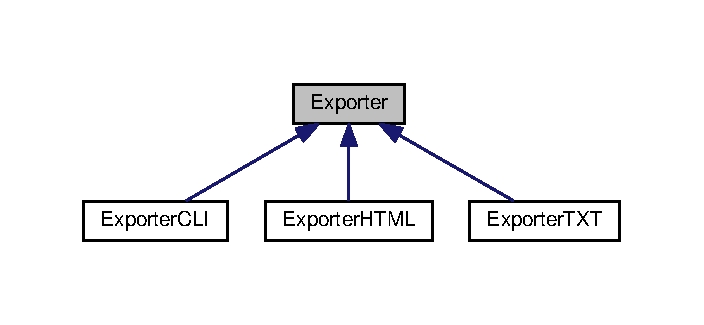
\includegraphics[width=350pt]{class_exporter__inherit__graph}
\end{center}
\end{figure}


Collaboration diagram for Exporter\+:
\nopagebreak
\begin{figure}[H]
\begin{center}
\leavevmode
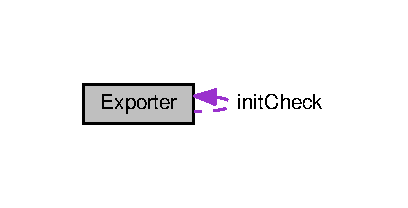
\includegraphics[width=204pt]{class_exporter__coll__graph}
\end{center}
\end{figure}
\subsection*{Public Member Functions}
\begin{DoxyCompactItemize}
\item 
\hyperlink{class_exporter_a2a977cb5ac8f637fcb570e73f650eca0}{Exporter} ()
\begin{DoxyCompactList}\small\item\em Lege constructor van \hyperlink{class_exporter}{Exporter}. \end{DoxyCompactList}\item 
bool \hyperlink{class_exporter_afba4e69e23ad018c26b21c0f4b85ef12}{is\+Document\+Started} () const 
\begin{DoxyCompactList}\small\item\em Getter van member document\+Started. \end{DoxyCompactList}\item 
virtual bool \hyperlink{class_exporter_af01d2a6c2f54329b1867a19537e11a34}{properly\+Initialised} () const 
\begin{DoxyCompactList}\small\item\em Kijk na of de constructor in de juiste staat geeindigd is. \end{DoxyCompactList}\item 
virtual void \hyperlink{class_exporter_ab3736803133eb727cf87a7306f91eb11}{write} (std\+::string \&output, std\+::ostream \&os)
\begin{DoxyCompactList}\small\item\em Stuur de output string naar de output stream. \end{DoxyCompactList}\item 
virtual void \hyperlink{class_exporter_ae477714f462d70cfc5b3970f91fcc4ed}{finish} (std\+::ostream \&os)
\begin{DoxyCompactList}\small\item\em Stuurt de nodige informatie naar de output stream om het document correct af te sluiten. \end{DoxyCompactList}\end{DoxyCompactItemize}
\subsection*{Protected Attributes}
\begin{DoxyCompactItemize}
\item 
bool \hyperlink{class_exporter_a7d55f6023d5fe983512f6b02fb60733b}{document\+Started}
\item 
\hyperlink{class_exporter}{Exporter} $\ast$ \hyperlink{class_exporter_a74245e988d8e72a43704dda927acff05}{init\+Check}
\end{DoxyCompactItemize}


\subsection{Detailed Description}
\hyperlink{class_exporter}{Exporter} base klasse die de output van gegevens behandelt. 

\subsection{Constructor \& Destructor Documentation}
\index{Exporter@{Exporter}!Exporter@{Exporter}}
\index{Exporter@{Exporter}!Exporter@{Exporter}}
\subsubsection[{\texorpdfstring{Exporter()}{Exporter()}}]{\setlength{\rightskip}{0pt plus 5cm}Exporter\+::\+Exporter (
\begin{DoxyParamCaption}
{}
\end{DoxyParamCaption}
)}\hypertarget{class_exporter_a2a977cb5ac8f637fcb570e73f650eca0}{}\label{class_exporter_a2a977cb5ac8f637fcb570e73f650eca0}


Lege constructor van \hyperlink{class_exporter}{Exporter}. 



\subsection{Member Function Documentation}
\index{Exporter@{Exporter}!finish@{finish}}
\index{finish@{finish}!Exporter@{Exporter}}
\subsubsection[{\texorpdfstring{finish(std\+::ostream \&os)}{finish(std::ostream &os)}}]{\setlength{\rightskip}{0pt plus 5cm}void Exporter\+::finish (
\begin{DoxyParamCaption}
\item[{std\+::ostream \&}]{os}
\end{DoxyParamCaption}
)\hspace{0.3cm}{\ttfamily [virtual]}}\hypertarget{class_exporter_ae477714f462d70cfc5b3970f91fcc4ed}{}\label{class_exporter_ae477714f462d70cfc5b3970f91fcc4ed}


Stuurt de nodige informatie naar de output stream om het document correct af te sluiten. 


\begin{DoxyParams}{Parameters}
{\em os} & De stream waar de output naar gestuurd zal worden. \\
\hline
\end{DoxyParams}
\begin{DoxyPrecond}{Precondition}
R\+E\+Q\+U\+I\+RE(this-\/$>$\hyperlink{class_exporter_af01d2a6c2f54329b1867a19537e11a34}{properly\+Initialised()}, \char`\"{}\+Exporter was niet geinitialiseerd bij de aanroep van finish.\char`\"{}); 

R\+E\+Q\+U\+I\+RE(document\+Started, \char`\"{}\+Document was niet aangemaakt voor de aanroep van finish.\char`\"{}); 
\end{DoxyPrecond}


Reimplemented in \hyperlink{class_exporter_h_t_m_l_aefa1c658f3c3c55bd7725bdad09629b3}{Exporter\+H\+T\+ML}.



Here is the call graph for this function\+:
\nopagebreak
\begin{figure}[H]
\begin{center}
\leavevmode
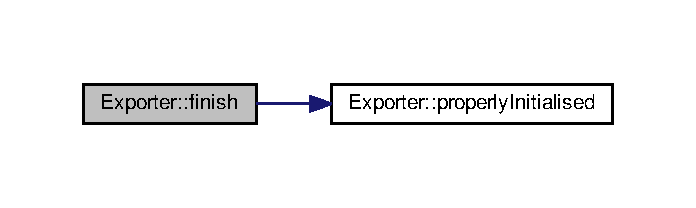
\includegraphics[width=350pt]{class_exporter_ae477714f462d70cfc5b3970f91fcc4ed_cgraph}
\end{center}
\end{figure}




Here is the caller graph for this function\+:
\nopagebreak
\begin{figure}[H]
\begin{center}
\leavevmode
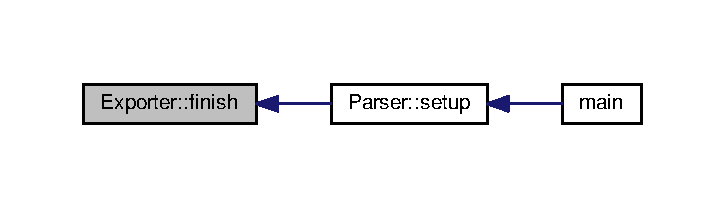
\includegraphics[width=263pt]{class_exporter_ae477714f462d70cfc5b3970f91fcc4ed_icgraph}
\end{center}
\end{figure}


\index{Exporter@{Exporter}!is\+Document\+Started@{is\+Document\+Started}}
\index{is\+Document\+Started@{is\+Document\+Started}!Exporter@{Exporter}}
\subsubsection[{\texorpdfstring{is\+Document\+Started() const }{isDocumentStarted() const }}]{\setlength{\rightskip}{0pt plus 5cm}bool Exporter\+::is\+Document\+Started (
\begin{DoxyParamCaption}
{}
\end{DoxyParamCaption}
) const}\hypertarget{class_exporter_afba4e69e23ad018c26b21c0f4b85ef12}{}\label{class_exporter_afba4e69e23ad018c26b21c0f4b85ef12}


Getter van member document\+Started. 

\begin{DoxyReturn}{Returns}
De waarde van document\+Started 
\end{DoxyReturn}
\begin{DoxyPrecond}{Precondition}
R\+E\+Q\+U\+I\+RE(this-\/$>$\hyperlink{class_exporter_af01d2a6c2f54329b1867a19537e11a34}{properly\+Initialised()}, \char`\"{}\+Exporter was niet geinitialiseerd bij de aanroep van is\+Document\+Started.\char`\"{}); 
\end{DoxyPrecond}


Here is the call graph for this function\+:
\nopagebreak
\begin{figure}[H]
\begin{center}
\leavevmode
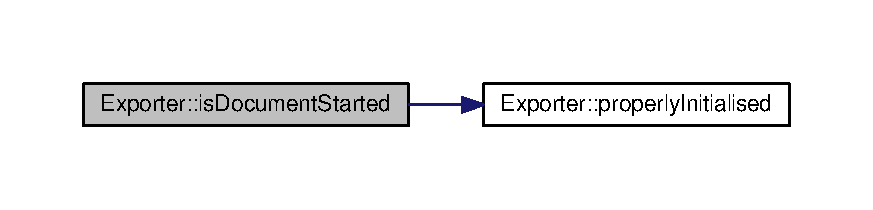
\includegraphics[width=350pt]{class_exporter_afba4e69e23ad018c26b21c0f4b85ef12_cgraph}
\end{center}
\end{figure}




Here is the caller graph for this function\+:
\nopagebreak
\begin{figure}[H]
\begin{center}
\leavevmode
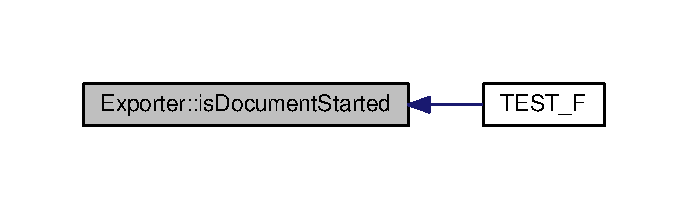
\includegraphics[width=330pt]{class_exporter_afba4e69e23ad018c26b21c0f4b85ef12_icgraph}
\end{center}
\end{figure}


\index{Exporter@{Exporter}!properly\+Initialised@{properly\+Initialised}}
\index{properly\+Initialised@{properly\+Initialised}!Exporter@{Exporter}}
\subsubsection[{\texorpdfstring{properly\+Initialised() const }{properlyInitialised() const }}]{\setlength{\rightskip}{0pt plus 5cm}bool Exporter\+::properly\+Initialised (
\begin{DoxyParamCaption}
{}
\end{DoxyParamCaption}
) const\hspace{0.3cm}{\ttfamily [virtual]}}\hypertarget{class_exporter_af01d2a6c2f54329b1867a19537e11a34}{}\label{class_exporter_af01d2a6c2f54329b1867a19537e11a34}


Kijk na of de constructor in de juiste staat geeindigd is. 

\begin{DoxyReturn}{Returns}
Boolean die aangeeft of het object juist geinitialiseerd is. 
\end{DoxyReturn}


Here is the caller graph for this function\+:
\nopagebreak
\begin{figure}[H]
\begin{center}
\leavevmode
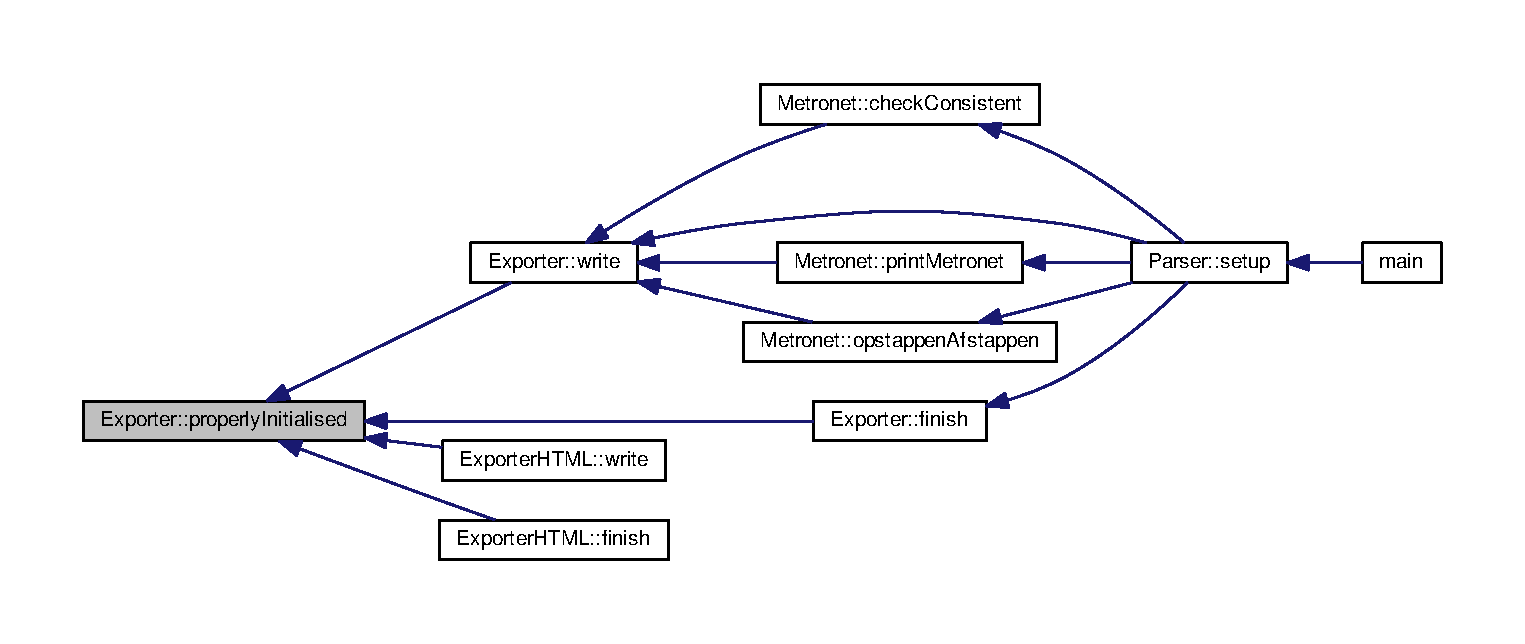
\includegraphics[width=350pt]{class_exporter_af01d2a6c2f54329b1867a19537e11a34_icgraph}
\end{center}
\end{figure}


\index{Exporter@{Exporter}!write@{write}}
\index{write@{write}!Exporter@{Exporter}}
\subsubsection[{\texorpdfstring{write(std\+::string \&output, std\+::ostream \&os)}{write(std::string &output, std::ostream &os)}}]{\setlength{\rightskip}{0pt plus 5cm}void Exporter\+::write (
\begin{DoxyParamCaption}
\item[{std\+::string \&}]{output, }
\item[{std\+::ostream \&}]{os}
\end{DoxyParamCaption}
)\hspace{0.3cm}{\ttfamily [virtual]}}\hypertarget{class_exporter_ab3736803133eb727cf87a7306f91eb11}{}\label{class_exporter_ab3736803133eb727cf87a7306f91eb11}


Stuur de output string naar de output stream. 


\begin{DoxyParams}{Parameters}
{\em output} & De string die naar de output gestuurd moet worden. \\
\hline
{\em os} & De stream waar de output naar gestuurd zal worden. \\
\hline
\end{DoxyParams}
\begin{DoxyPrecond}{Precondition}
R\+E\+Q\+U\+I\+RE(this-\/$>$\hyperlink{class_exporter_af01d2a6c2f54329b1867a19537e11a34}{properly\+Initialised()}, \char`\"{}\+Exporter was niet geinitialiseerd bij de aanroep van write.\char`\"{}); 
\end{DoxyPrecond}
\begin{DoxyPostcond}{Postcondition}
E\+N\+S\+U\+RE(document\+Started, \char`\"{}\+Document was niet aangemaakt bij de aanroep van write.\char`\"{}); 
\end{DoxyPostcond}


Reimplemented in \hyperlink{class_exporter_h_t_m_l_ace2649c240282289d4cb3bfbd19e427c}{Exporter\+H\+T\+ML}.



Here is the call graph for this function\+:
\nopagebreak
\begin{figure}[H]
\begin{center}
\leavevmode
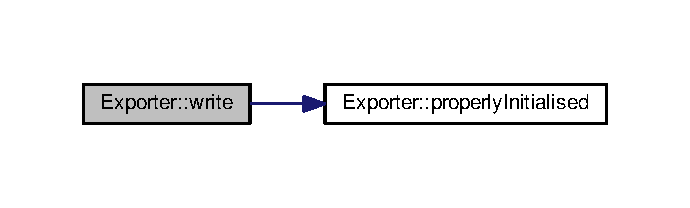
\includegraphics[width=350pt]{class_exporter_ab3736803133eb727cf87a7306f91eb11_cgraph}
\end{center}
\end{figure}




Here is the caller graph for this function\+:
\nopagebreak
\begin{figure}[H]
\begin{center}
\leavevmode
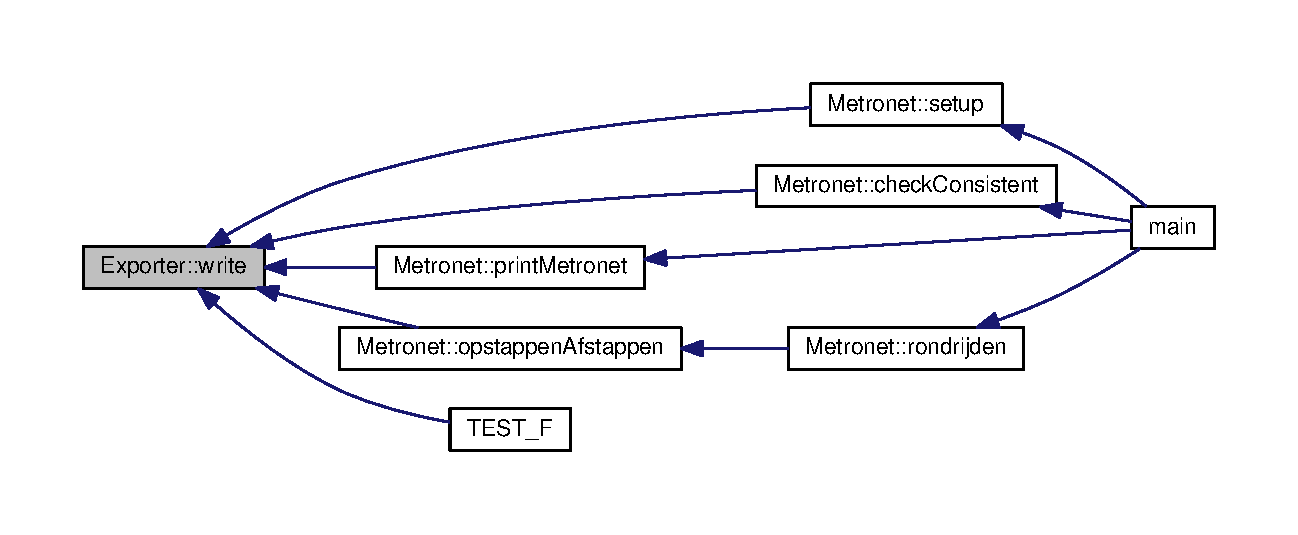
\includegraphics[width=350pt]{class_exporter_ab3736803133eb727cf87a7306f91eb11_icgraph}
\end{center}
\end{figure}




\subsection{Member Data Documentation}
\index{Exporter@{Exporter}!document\+Started@{document\+Started}}
\index{document\+Started@{document\+Started}!Exporter@{Exporter}}
\subsubsection[{\texorpdfstring{document\+Started}{documentStarted}}]{\setlength{\rightskip}{0pt plus 5cm}bool Exporter\+::document\+Started\hspace{0.3cm}{\ttfamily [protected]}}\hypertarget{class_exporter_a7d55f6023d5fe983512f6b02fb60733b}{}\label{class_exporter_a7d55f6023d5fe983512f6b02fb60733b}
\index{Exporter@{Exporter}!init\+Check@{init\+Check}}
\index{init\+Check@{init\+Check}!Exporter@{Exporter}}
\subsubsection[{\texorpdfstring{init\+Check}{initCheck}}]{\setlength{\rightskip}{0pt plus 5cm}{\bf Exporter}$\ast$ Exporter\+::init\+Check\hspace{0.3cm}{\ttfamily [protected]}}\hypertarget{class_exporter_a74245e988d8e72a43704dda927acff05}{}\label{class_exporter_a74245e988d8e72a43704dda927acff05}


The documentation for this class was generated from the following files\+:\begin{DoxyCompactItemize}
\item 
/home/jonathan/\+Desktop/\+Project Software Engineering/\+Metronet/\+P\+S\+E/src/\hyperlink{_exporter_8h}{Exporter.\+h}\item 
/home/jonathan/\+Desktop/\+Project Software Engineering/\+Metronet/\+P\+S\+E/src/\hyperlink{_exporter_8cpp}{Exporter.\+cpp}\end{DoxyCompactItemize}

\hypertarget{class_exporter_c_l_i}{}\section{Exporter\+C\+LI Class Reference}
\label{class_exporter_c_l_i}\index{Exporter\+C\+LI@{Exporter\+C\+LI}}


{\ttfamily \#include $<$Exporter.\+h$>$}



Inheritance diagram for Exporter\+C\+LI\+:\nopagebreak
\begin{figure}[H]
\begin{center}
\leavevmode
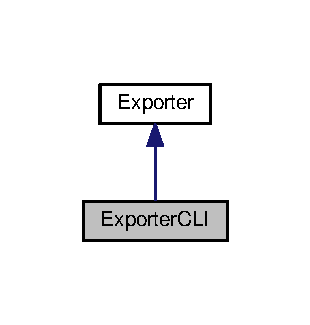
\includegraphics[width=149pt]{class_exporter_c_l_i__inherit__graph}
\end{center}
\end{figure}


Collaboration diagram for Exporter\+C\+LI\+:\nopagebreak
\begin{figure}[H]
\begin{center}
\leavevmode
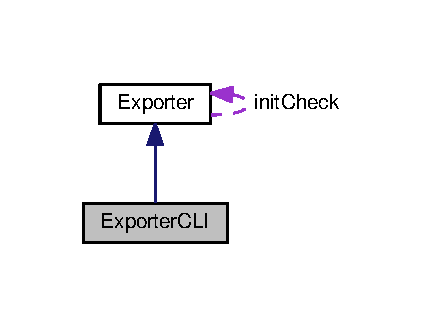
\includegraphics[width=204pt]{class_exporter_c_l_i__coll__graph}
\end{center}
\end{figure}
\subsection*{Additional Inherited Members}


The documentation for this class was generated from the following file\+:\begin{DoxyCompactItemize}
\item 
/home/jonathan/\+Desktop/\+Project Software Engineering/\+Metronet/\+P\+S\+E/src/\hyperlink{_exporter_8h}{Exporter.\+h}\end{DoxyCompactItemize}

\hypertarget{class_exporter_h_t_m_l}{}\section{Exporter\+H\+T\+ML Class Reference}
\label{class_exporter_h_t_m_l}\index{Exporter\+H\+T\+ML@{Exporter\+H\+T\+ML}}


{\ttfamily \#include $<$Exporter.\+h$>$}



Inheritance diagram for Exporter\+H\+T\+ML\+:
\nopagebreak
\begin{figure}[H]
\begin{center}
\leavevmode
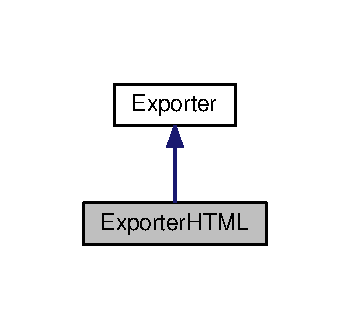
\includegraphics[width=160pt]{class_exporter_h_t_m_l__inherit__graph}
\end{center}
\end{figure}


Collaboration diagram for Exporter\+H\+T\+ML\+:
\nopagebreak
\begin{figure}[H]
\begin{center}
\leavevmode
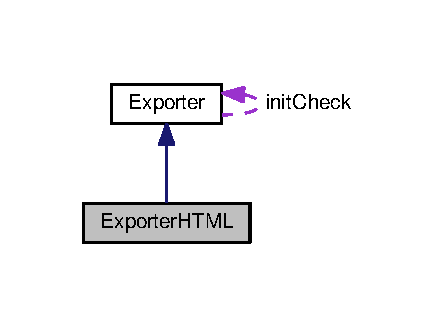
\includegraphics[width=160pt]{class_exporter_h_t_m_l__coll__graph}
\end{center}
\end{figure}
\subsection*{Public Member Functions}
\begin{DoxyCompactItemize}
\item 
virtual void \hyperlink{class_exporter_h_t_m_l_aa5b12621501f09a9a082e9337fbf943c}{write} (std\+::string \&output)
\begin{DoxyCompactList}\small\item\em Stuur de output string naar de output stream. \end{DoxyCompactList}\item 
virtual void \hyperlink{class_exporter_h_t_m_l_a60518b938e3cddd92ce3218de3651ac4}{validate} ()
\begin{DoxyCompactList}\small\item\em Valideer de output formaat. \end{DoxyCompactList}\item 
void \hyperlink{class_exporter_h_t_m_l_a2d9bb5e5f68a9e6111d8a929eb4a042e}{validate\+Head} ()
\begin{DoxyCompactList}\small\item\em Valideer de H\+T\+ML header. \end{DoxyCompactList}\item 
void \hyperlink{class_exporter_h_t_m_l_ab9d3ebcfa054f02f08ab34e1a6298963}{validate\+Tail} ()
\begin{DoxyCompactList}\small\item\em Valideer de H\+T\+ML tail. \end{DoxyCompactList}\end{DoxyCompactItemize}


\subsection{Member Function Documentation}
\index{Exporter\+H\+T\+ML@{Exporter\+H\+T\+ML}!validate@{validate}}
\index{validate@{validate}!Exporter\+H\+T\+ML@{Exporter\+H\+T\+ML}}
\subsubsection[{\texorpdfstring{validate()}{validate()}}]{\setlength{\rightskip}{0pt plus 5cm}void Exporter\+H\+T\+M\+L\+::validate (
\begin{DoxyParamCaption}
{}
\end{DoxyParamCaption}
)\hspace{0.3cm}{\ttfamily [virtual]}}\hypertarget{class_exporter_h_t_m_l_a60518b938e3cddd92ce3218de3651ac4}{}\label{class_exporter_h_t_m_l_a60518b938e3cddd92ce3218de3651ac4}


Valideer de output formaat. 

R\+E\+Q\+U\+I\+RE(this-\/$>$\hyperlink{class_exporter_af01d2a6c2f54329b1867a19537e11a34}{properly\+Initialised()}, \char`\"{}\+Exporter was niet geinitialiseerd bij de aanroep van validate,\char`\"{});~\newline
E\+N\+S\+U\+RE((document\+Started == true), \char`\"{}\+Document werd niet aangemaakt bij de aanroep van validate.\char`\"{});~\newline


Reimplemented from \hyperlink{class_exporter_a190fe737bcda2a55707ae51b731d11a5}{Exporter}.



Here is the call graph for this function\+:
\nopagebreak
\begin{figure}[H]
\begin{center}
\leavevmode
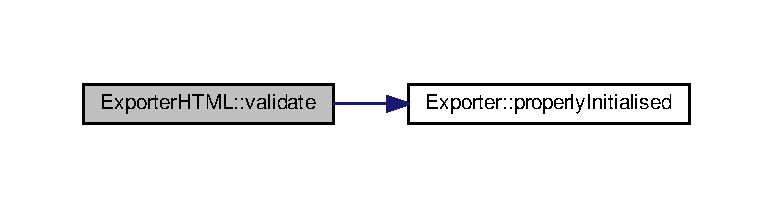
\includegraphics[width=350pt]{class_exporter_h_t_m_l_a60518b938e3cddd92ce3218de3651ac4_cgraph}
\end{center}
\end{figure}


\index{Exporter\+H\+T\+ML@{Exporter\+H\+T\+ML}!validate\+Head@{validate\+Head}}
\index{validate\+Head@{validate\+Head}!Exporter\+H\+T\+ML@{Exporter\+H\+T\+ML}}
\subsubsection[{\texorpdfstring{validate\+Head()}{validateHead()}}]{\setlength{\rightskip}{0pt plus 5cm}void Exporter\+H\+T\+M\+L\+::validate\+Head (
\begin{DoxyParamCaption}
{}
\end{DoxyParamCaption}
)}\hypertarget{class_exporter_h_t_m_l_a2d9bb5e5f68a9e6111d8a929eb4a042e}{}\label{class_exporter_h_t_m_l_a2d9bb5e5f68a9e6111d8a929eb4a042e}


Valideer de H\+T\+ML header. 

R\+E\+Q\+U\+I\+RE(this-\/$>$\hyperlink{class_exporter_af01d2a6c2f54329b1867a19537e11a34}{properly\+Initialised()}, \char`\"{}\+Exporter\+H\+T\+M\+L was niet geinitialiseerd bij het aanroepen van validate\+Head.\char`\"{});~\newline
R\+E\+Q\+U\+I\+RE(document\+Started == false), \char`\"{}\+Document was al aangemaakt voor de aanroep van validate\+Head.\char`\"{});~\newline
E\+N\+S\+U\+RE((document\+Started == true), \char`\"{}\+Document werd niet aangemaakt bij de aanroep van validate\+Head.\char`\"{});~\newline


Here is the call graph for this function\+:
\nopagebreak
\begin{figure}[H]
\begin{center}
\leavevmode
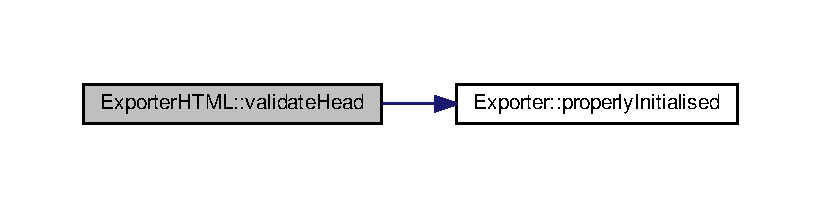
\includegraphics[width=350pt]{class_exporter_h_t_m_l_a2d9bb5e5f68a9e6111d8a929eb4a042e_cgraph}
\end{center}
\end{figure}


\index{Exporter\+H\+T\+ML@{Exporter\+H\+T\+ML}!validate\+Tail@{validate\+Tail}}
\index{validate\+Tail@{validate\+Tail}!Exporter\+H\+T\+ML@{Exporter\+H\+T\+ML}}
\subsubsection[{\texorpdfstring{validate\+Tail()}{validateTail()}}]{\setlength{\rightskip}{0pt plus 5cm}void Exporter\+H\+T\+M\+L\+::validate\+Tail (
\begin{DoxyParamCaption}
{}
\end{DoxyParamCaption}
)}\hypertarget{class_exporter_h_t_m_l_ab9d3ebcfa054f02f08ab34e1a6298963}{}\label{class_exporter_h_t_m_l_ab9d3ebcfa054f02f08ab34e1a6298963}


Valideer de H\+T\+ML tail. 

R\+E\+Q\+U\+I\+RE(this-\/$>$\hyperlink{class_exporter_af01d2a6c2f54329b1867a19537e11a34}{properly\+Initialised()}, \char`\"{}\+Exporter\+H\+T\+M\+L was niet geinitialiseerd bij het aanroepen van validate\+Tail.\char`\"{});~\newline
R\+E\+Q\+U\+I\+RE((document\+Started == true), \char`\"{}\+Document was nog niet aangemaakt bij de aanroep van validate\+Tail.\char`\"{}); E\+N\+S\+U\+RE((document\+Started == true), \char`\"{}\+Document werd niet aangemaakt bij de aanroep van validate\+Tail.\char`\"{});.~\newline


Here is the call graph for this function\+:
\nopagebreak
\begin{figure}[H]
\begin{center}
\leavevmode
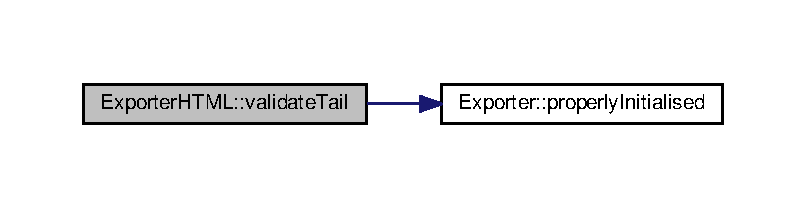
\includegraphics[width=350pt]{class_exporter_h_t_m_l_ab9d3ebcfa054f02f08ab34e1a6298963_cgraph}
\end{center}
\end{figure}


\index{Exporter\+H\+T\+ML@{Exporter\+H\+T\+ML}!write@{write}}
\index{write@{write}!Exporter\+H\+T\+ML@{Exporter\+H\+T\+ML}}
\subsubsection[{\texorpdfstring{write(std\+::string \&output)}{write(std::string &output)}}]{\setlength{\rightskip}{0pt plus 5cm}void Exporter\+H\+T\+M\+L\+::write (
\begin{DoxyParamCaption}
\item[{std\+::string \&}]{output}
\end{DoxyParamCaption}
)\hspace{0.3cm}{\ttfamily [virtual]}}\hypertarget{class_exporter_h_t_m_l_aa5b12621501f09a9a082e9337fbf943c}{}\label{class_exporter_h_t_m_l_aa5b12621501f09a9a082e9337fbf943c}


Stuur de output string naar de output stream. 


\begin{DoxyParams}{Parameters}
{\em output} & De string die naar de output gestuurd moet worden.\\
\hline
\end{DoxyParams}
R\+E\+Q\+U\+I\+RE(this-\/$>$\hyperlink{class_exporter_af01d2a6c2f54329b1867a19537e11a34}{properly\+Initialised()}, \char`\"{}\+Exporter was niet geinitialiseerd bij de aanroep van write.\char`\"{});~\newline


Reimplemented from \hyperlink{class_exporter_ac095b6486da16ffc76539f8c6c67be70}{Exporter}.



Here is the call graph for this function\+:
\nopagebreak
\begin{figure}[H]
\begin{center}
\leavevmode
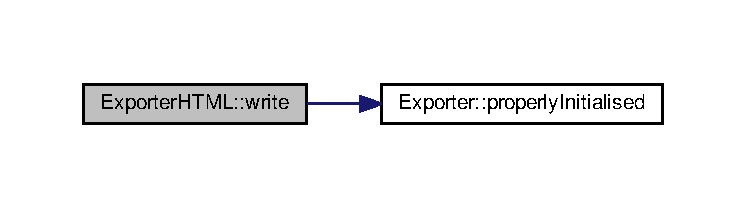
\includegraphics[width=350pt]{class_exporter_h_t_m_l_aa5b12621501f09a9a082e9337fbf943c_cgraph}
\end{center}
\end{figure}




The documentation for this class was generated from the following files\+:\begin{DoxyCompactItemize}
\item 
/home/jonathan/\+Desktop/\+Project Software Engineering/\+Metronet/\+P\+S\+E/src/\hyperlink{_exporter_8h}{Exporter.\+h}\item 
/home/jonathan/\+Desktop/\+Project Software Engineering/\+Metronet/\+P\+S\+E/src/\hyperlink{_exporter_8cpp}{Exporter.\+cpp}\end{DoxyCompactItemize}

\hypertarget{class_exporter_t_x_t}{}\section{Exporter\+T\+XT Class Reference}
\label{class_exporter_t_x_t}\index{Exporter\+T\+XT@{Exporter\+T\+XT}}


{\ttfamily \#include $<$Exporter.\+h$>$}



Inheritance diagram for Exporter\+T\+XT\+:
\nopagebreak
\begin{figure}[H]
\begin{center}
\leavevmode
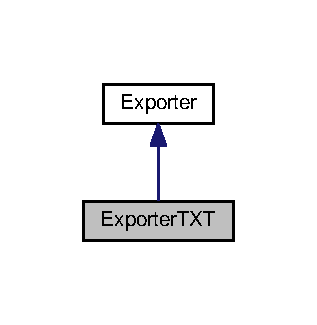
\includegraphics[width=152pt]{class_exporter_t_x_t__inherit__graph}
\end{center}
\end{figure}


Collaboration diagram for Exporter\+T\+XT\+:
\nopagebreak
\begin{figure}[H]
\begin{center}
\leavevmode
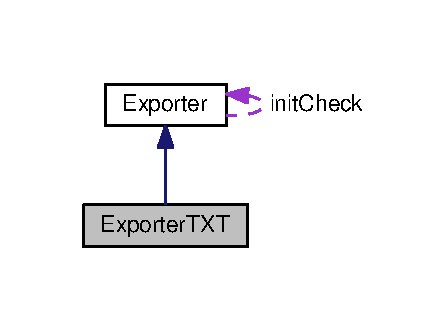
\includegraphics[width=152pt]{class_exporter_t_x_t__coll__graph}
\end{center}
\end{figure}
\subsection*{Additional Inherited Members}


The documentation for this class was generated from the following file\+:\begin{DoxyCompactItemize}
\item 
/home/jonathan/\+Desktop/\+Project Software Engineering/\+Metronet/\+P\+S\+E/src/\hyperlink{_exporter_8h}{Exporter.\+h}\end{DoxyCompactItemize}

\hypertarget{class_metronet}{}\section{Metronet Class Reference}
\label{class_metronet}\index{Metronet@{Metronet}}
\subsection*{Public Member Functions}
\begin{DoxyCompactItemize}
\item 
\mbox{\Hypertarget{class_metronet_a3d2adce29a947f162924279b766de645}\label{class_metronet_a3d2adce29a947f162924279b766de645}} 
bool \hyperlink{class_metronet_a3d2adce29a947f162924279b766de645}{properly\+Initialised} ()
\begin{DoxyCompactList}\small\item\em Kijk na of de constructor in de juiste staat geeindigd is. \end{DoxyCompactList}\item 
void \hyperlink{class_metronet_a37106294bf52324b0fb9fcecf11e5495}{add\+Station} (\hyperlink{class_station}{Station} $\ast$)
\begin{DoxyCompactList}\small\item\em Voegt station toe aan metronet. \end{DoxyCompactList}\item 
void \hyperlink{class_metronet_ab9bcc898b7b0ec5571ce149364cf64fc}{add\+Tram} (\hyperlink{class_tram}{Tram} $\ast$)
\begin{DoxyCompactList}\small\item\em Voegt tram toe aan metronet. \end{DoxyCompactList}\item 
void \hyperlink{class_metronet_ab6faa9e35828352e4003640d13798529}{add\+Spoor} (\hyperlink{class_spoor}{Spoor} $\ast$)
\begin{DoxyCompactList}\small\item\em Voegt spoor toe aan metronet. \end{DoxyCompactList}\item 
bool \hyperlink{class_metronet_a0128de167ec0a36e70abd57170b3faed}{check\+Consistent} (\hyperlink{class_exporter}{Exporter} $\ast$exp)
\begin{DoxyCompactList}\small\item\em Kijkt na of het metronet consistent is. \end{DoxyCompactList}\end{DoxyCompactItemize}


\subsection{Member Function Documentation}
\mbox{\Hypertarget{class_metronet_ab6faa9e35828352e4003640d13798529}\label{class_metronet_ab6faa9e35828352e4003640d13798529}} 
\index{Metronet@{Metronet}!add\+Spoor@{add\+Spoor}}
\index{add\+Spoor@{add\+Spoor}!Metronet@{Metronet}}
\subsubsection{\texorpdfstring{add\+Spoor()}{addSpoor()}}
{\footnotesize\ttfamily void Metronet\+::add\+Spoor (\begin{DoxyParamCaption}\item[{\hyperlink{class_spoor}{Spoor} $\ast$}]{spoor }\end{DoxyParamCaption})}



Voegt spoor toe aan metronet. 

R\+E\+Q\+U\+I\+RE(this-\/$>$\hyperlink{class_metronet_a3d2adce29a947f162924279b766de645}{properly\+Initialised()}, \char`\"{}\+Metronet was niet geinitialiseerd bij de aanroep van add\+Spoor.\char`\"{});~\newline
R\+E\+Q\+U\+I\+RE(Spoor-\/$>$\hyperlink{class_metronet_a3d2adce29a947f162924279b766de645}{properly\+Initialised()}, \char`\"{}\+Spoor was niet geinitialiseerd bij de aanroep van add\+Spoor.\char`\"{});~\newline
E\+N\+S\+U\+RE(sporen\mbox{[}sporen.\+size() -\/ 1\mbox{]} == \hyperlink{class_spoor}{Spoor}), \char`\"{}\+Spoor was niet toegevoegd bij de aanroep van add\+Spoor.\char`\"{});~\newline
\mbox{\Hypertarget{class_metronet_a37106294bf52324b0fb9fcecf11e5495}\label{class_metronet_a37106294bf52324b0fb9fcecf11e5495}} 
\index{Metronet@{Metronet}!add\+Station@{add\+Station}}
\index{add\+Station@{add\+Station}!Metronet@{Metronet}}
\subsubsection{\texorpdfstring{add\+Station()}{addStation()}}
{\footnotesize\ttfamily void Metronet\+::add\+Station (\begin{DoxyParamCaption}\item[{\hyperlink{class_station}{Station} $\ast$}]{station }\end{DoxyParamCaption})}



Voegt station toe aan metronet. 

R\+E\+Q\+U\+I\+RE(this-\/$>$\hyperlink{class_metronet_a3d2adce29a947f162924279b766de645}{properly\+Initialised()}, \char`\"{}\+Metronet was niet geinitialiseerd bij de aanroep van add\+Station.\char`\"{});~\newline
R\+E\+Q\+U\+I\+RE(Station-\/$>$\hyperlink{class_metronet_a3d2adce29a947f162924279b766de645}{properly\+Initialised()}, \char`\"{}\+Station was niet geinitialiseerd bij de aanroep van add\+Station.\char`\"{});~\newline
E\+N\+S\+U\+RE(stations\mbox{[}stations.\+size() -\/ 1\mbox{]} == \hyperlink{class_station}{Station}), \char`\"{}\+Station was niet toegevoegd bij de aanroep van add\+Station.\char`\"{});~\newline
\mbox{\Hypertarget{class_metronet_ab9bcc898b7b0ec5571ce149364cf64fc}\label{class_metronet_ab9bcc898b7b0ec5571ce149364cf64fc}} 
\index{Metronet@{Metronet}!add\+Tram@{add\+Tram}}
\index{add\+Tram@{add\+Tram}!Metronet@{Metronet}}
\subsubsection{\texorpdfstring{add\+Tram()}{addTram()}}
{\footnotesize\ttfamily void Metronet\+::add\+Tram (\begin{DoxyParamCaption}\item[{\hyperlink{class_tram}{Tram} $\ast$}]{tram }\end{DoxyParamCaption})}



Voegt tram toe aan metronet. 

R\+E\+Q\+U\+I\+RE(this-\/$>$\hyperlink{class_metronet_a3d2adce29a947f162924279b766de645}{properly\+Initialised()}, \char`\"{}\+Metronet was niet geinitialiseerd bij de aanroep van add\+Tram.\char`\"{});~\newline
R\+E\+Q\+U\+I\+RE(Tram-\/$>$\hyperlink{class_metronet_a3d2adce29a947f162924279b766de645}{properly\+Initialised()}, \char`\"{}\+Tram was niet geinitialiseerd bij de aanroep van add\+Tram.\char`\"{});~\newline
E\+N\+S\+U\+RE(trams\mbox{[}trams.\+size() -\/ 1\mbox{]} == \hyperlink{class_tram}{Tram}), \char`\"{}\+Tram was niet toegevoegd bij de aanroep van add\+Tram.\char`\"{});~\newline
\mbox{\Hypertarget{class_metronet_a0128de167ec0a36e70abd57170b3faed}\label{class_metronet_a0128de167ec0a36e70abd57170b3faed}} 
\index{Metronet@{Metronet}!check\+Consistent@{check\+Consistent}}
\index{check\+Consistent@{check\+Consistent}!Metronet@{Metronet}}
\subsubsection{\texorpdfstring{check\+Consistent()}{checkConsistent()}}
{\footnotesize\ttfamily bool Metronet\+::check\+Consistent (\begin{DoxyParamCaption}\item[{\hyperlink{class_exporter}{Exporter} $\ast$}]{exp }\end{DoxyParamCaption})}



Kijkt na of het metronet consistent is. 


\begin{DoxyParams}{Parameters}
{\em exp} & De exporter die de output zal behandelen. R\+E\+Q\+U\+I\+RE(this-\/$>$\hyperlink{class_metronet_a3d2adce29a947f162924279b766de645}{properly\+Initialised()}, \char`\"{}\+Metronet was niet geinitialiseerd bij de aanroep van check\+Consistent.\char`\"{});~\newline
\\
\hline
\end{DoxyParams}


The documentation for this class was generated from the following files\+:\begin{DoxyCompactItemize}
\item 
/home/sergio/\+C\+Lion\+Projects/\+Soft\+Eng/src/Metronet.\+h\item 
/home/sergio/\+C\+Lion\+Projects/\+Soft\+Eng/src/Metronet.\+cpp\end{DoxyCompactItemize}

\hypertarget{class_metronet_domain_test}{}\section{Metronet\+Domain\+Test Class Reference}
\label{class_metronet_domain_test}\index{Metronet\+Domain\+Test@{Metronet\+Domain\+Test}}


\hyperlink{class_metronet_domain_test}{Metronet\+Domain\+Test} klasse die domein tests behandelt.  




{\ttfamily \#include $<$Metronet\+Domain\+Test.\+h$>$}



Inheritance diagram for Metronet\+Domain\+Test\+:\nopagebreak
\begin{figure}[H]
\begin{center}
\leavevmode
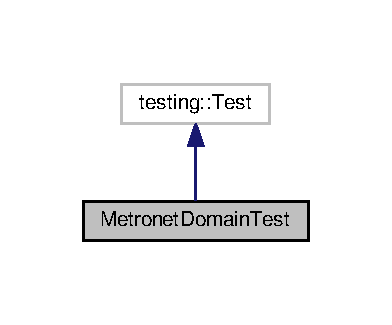
\includegraphics[width=188pt]{class_metronet_domain_test__inherit__graph}
\end{center}
\end{figure}


Collaboration diagram for Metronet\+Domain\+Test\+:
\nopagebreak
\begin{figure}[H]
\begin{center}
\leavevmode
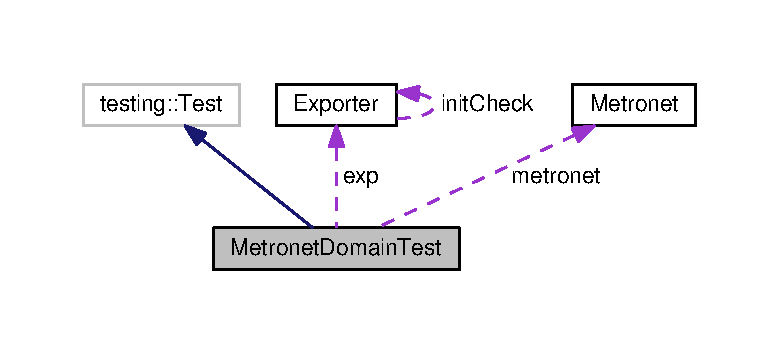
\includegraphics[width=350pt]{class_metronet_domain_test__coll__graph}
\end{center}
\end{figure}
\subsection*{Protected Member Functions}
\begin{DoxyCompactItemize}
\item 
virtual void \hyperlink{class_metronet_domain_test_ac8e8d15b45d53810c4427084fad6388f}{Set\+Up} ()
\item 
virtual void \hyperlink{class_metronet_domain_test_a3429b373771815652c80d013f81369a0}{Tear\+Down} ()
\end{DoxyCompactItemize}
\subsection*{Protected Attributes}
\begin{DoxyCompactItemize}
\item 
\hyperlink{class_metronet}{Metronet} \hyperlink{class_metronet_domain_test_aa185f99af6607124a6fea8c4f63fddb7}{metronet}
\item 
\hyperlink{class_exporter}{Exporter} $\ast$ \hyperlink{class_metronet_domain_test_a6e7c903d4485d95a766f8ff01989d529}{exp}
\end{DoxyCompactItemize}
\subsection*{Friends}
\begin{DoxyCompactItemize}
\item 
class \hyperlink{class_metronet_domain_test_a07c94fb69880743e62f64a941fc2d4ab}{Metronet}
\end{DoxyCompactItemize}


\subsection{Detailed Description}
\hyperlink{class_metronet_domain_test}{Metronet\+Domain\+Test} klasse die domein tests behandelt. 

\subsection{Member Function Documentation}
\mbox{\Hypertarget{class_metronet_domain_test_ac8e8d15b45d53810c4427084fad6388f}\label{class_metronet_domain_test_ac8e8d15b45d53810c4427084fad6388f}} 
\index{Metronet\+Domain\+Test@{Metronet\+Domain\+Test}!Set\+Up@{Set\+Up}}
\index{Set\+Up@{Set\+Up}!Metronet\+Domain\+Test@{Metronet\+Domain\+Test}}
\subsubsection{\texorpdfstring{Set\+Up()}{SetUp()}}
{\footnotesize\ttfamily virtual void Metronet\+Domain\+Test\+::\+Set\+Up (\begin{DoxyParamCaption}{ }\end{DoxyParamCaption})\hspace{0.3cm}{\ttfamily [inline]}, {\ttfamily [protected]}, {\ttfamily [virtual]}}

\mbox{\Hypertarget{class_metronet_domain_test_a3429b373771815652c80d013f81369a0}\label{class_metronet_domain_test_a3429b373771815652c80d013f81369a0}} 
\index{Metronet\+Domain\+Test@{Metronet\+Domain\+Test}!Tear\+Down@{Tear\+Down}}
\index{Tear\+Down@{Tear\+Down}!Metronet\+Domain\+Test@{Metronet\+Domain\+Test}}
\subsubsection{\texorpdfstring{Tear\+Down()}{TearDown()}}
{\footnotesize\ttfamily virtual void Metronet\+Domain\+Test\+::\+Tear\+Down (\begin{DoxyParamCaption}{ }\end{DoxyParamCaption})\hspace{0.3cm}{\ttfamily [inline]}, {\ttfamily [protected]}, {\ttfamily [virtual]}}



\subsection{Friends And Related Function Documentation}
\mbox{\Hypertarget{class_metronet_domain_test_a07c94fb69880743e62f64a941fc2d4ab}\label{class_metronet_domain_test_a07c94fb69880743e62f64a941fc2d4ab}} 
\index{Metronet\+Domain\+Test@{Metronet\+Domain\+Test}!Metronet@{Metronet}}
\index{Metronet@{Metronet}!Metronet\+Domain\+Test@{Metronet\+Domain\+Test}}
\subsubsection{\texorpdfstring{Metronet}{Metronet}}
{\footnotesize\ttfamily friend class \hyperlink{class_metronet}{Metronet}\hspace{0.3cm}{\ttfamily [friend]}}



\subsection{Member Data Documentation}
\mbox{\Hypertarget{class_metronet_domain_test_a6e7c903d4485d95a766f8ff01989d529}\label{class_metronet_domain_test_a6e7c903d4485d95a766f8ff01989d529}} 
\index{Metronet\+Domain\+Test@{Metronet\+Domain\+Test}!exp@{exp}}
\index{exp@{exp}!Metronet\+Domain\+Test@{Metronet\+Domain\+Test}}
\subsubsection{\texorpdfstring{exp}{exp}}
{\footnotesize\ttfamily \hyperlink{class_exporter}{Exporter}$\ast$ Metronet\+Domain\+Test\+::exp\hspace{0.3cm}{\ttfamily [protected]}}

\mbox{\Hypertarget{class_metronet_domain_test_aa185f99af6607124a6fea8c4f63fddb7}\label{class_metronet_domain_test_aa185f99af6607124a6fea8c4f63fddb7}} 
\index{Metronet\+Domain\+Test@{Metronet\+Domain\+Test}!metronet@{metronet}}
\index{metronet@{metronet}!Metronet\+Domain\+Test@{Metronet\+Domain\+Test}}
\subsubsection{\texorpdfstring{metronet}{metronet}}
{\footnotesize\ttfamily \hyperlink{class_metronet}{Metronet} Metronet\+Domain\+Test\+::metronet\hspace{0.3cm}{\ttfamily [protected]}}



The documentation for this class was generated from the following file\+:\begin{DoxyCompactItemize}
\item 
/home/sergio/\+C\+Lion\+Projects/\+Soft\+Eng/src/\hyperlink{_metronet_domain_test_8h}{Metronet\+Domain\+Test.\+h}\end{DoxyCompactItemize}

\hypertarget{class_metronet_input_test}{}\section{Metronet\+Input\+Test Class Reference}
\label{class_metronet_input_test}\index{Metronet\+Input\+Test@{Metronet\+Input\+Test}}


{\ttfamily \#include $<$Metronet\+Input\+Test.\+h$>$}



Inheritance diagram for Metronet\+Input\+Test\+:\nopagebreak
\begin{figure}[H]
\begin{center}
\leavevmode
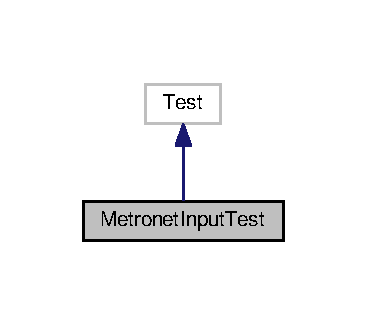
\includegraphics[width=176pt]{class_metronet_input_test__inherit__graph}
\end{center}
\end{figure}


Collaboration diagram for Metronet\+Input\+Test\+:\nopagebreak
\begin{figure}[H]
\begin{center}
\leavevmode
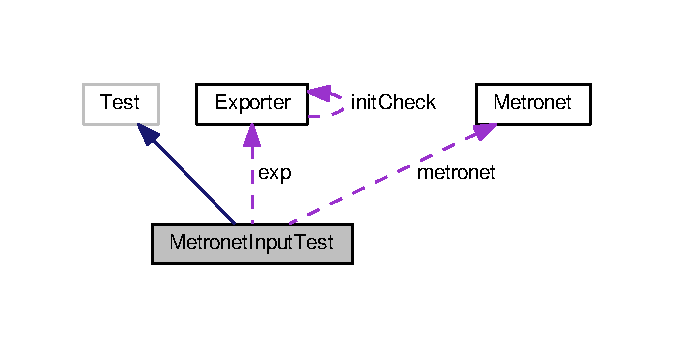
\includegraphics[width=324pt]{class_metronet_input_test__coll__graph}
\end{center}
\end{figure}
\subsection*{Protected Member Functions}
\begin{DoxyCompactItemize}
\item 
virtual void \hyperlink{class_metronet_input_test_a863299908a545656568a7d534387e05d}{Set\+Up} ()
\item 
virtual void \hyperlink{class_metronet_input_test_a20f35cb70be79eee36b1dab816cf6806}{Tear\+Down} ()
\end{DoxyCompactItemize}
\subsection*{Protected Attributes}
\begin{DoxyCompactItemize}
\item 
\hyperlink{class_metronet}{Metronet} \hyperlink{class_metronet_input_test_ab922ed7c2e4f1dfee1ed7df1eb3a13b4}{metronet}
\item 
\hyperlink{class_exporter}{Exporter} $\ast$ \hyperlink{class_metronet_input_test_ae16b3047e5801a34ef23dd9314e44770}{exp}
\end{DoxyCompactItemize}
\subsection*{Friends}
\begin{DoxyCompactItemize}
\item 
class \hyperlink{class_metronet_input_test_a07c94fb69880743e62f64a941fc2d4ab}{Metronet}
\end{DoxyCompactItemize}


\subsection{Member Function Documentation}
\index{Metronet\+Input\+Test@{Metronet\+Input\+Test}!Set\+Up@{Set\+Up}}
\index{Set\+Up@{Set\+Up}!Metronet\+Input\+Test@{Metronet\+Input\+Test}}
\subsubsection[{\texorpdfstring{Set\+Up()}{SetUp()}}]{\setlength{\rightskip}{0pt plus 5cm}virtual void Metronet\+Input\+Test\+::\+Set\+Up (
\begin{DoxyParamCaption}
{}
\end{DoxyParamCaption}
)\hspace{0.3cm}{\ttfamily [inline]}, {\ttfamily [protected]}, {\ttfamily [virtual]}}\hypertarget{class_metronet_input_test_a863299908a545656568a7d534387e05d}{}\label{class_metronet_input_test_a863299908a545656568a7d534387e05d}
\index{Metronet\+Input\+Test@{Metronet\+Input\+Test}!Tear\+Down@{Tear\+Down}}
\index{Tear\+Down@{Tear\+Down}!Metronet\+Input\+Test@{Metronet\+Input\+Test}}
\subsubsection[{\texorpdfstring{Tear\+Down()}{TearDown()}}]{\setlength{\rightskip}{0pt plus 5cm}virtual void Metronet\+Input\+Test\+::\+Tear\+Down (
\begin{DoxyParamCaption}
{}
\end{DoxyParamCaption}
)\hspace{0.3cm}{\ttfamily [inline]}, {\ttfamily [protected]}, {\ttfamily [virtual]}}\hypertarget{class_metronet_input_test_a20f35cb70be79eee36b1dab816cf6806}{}\label{class_metronet_input_test_a20f35cb70be79eee36b1dab816cf6806}


\subsection{Friends And Related Function Documentation}
\index{Metronet\+Input\+Test@{Metronet\+Input\+Test}!Metronet@{Metronet}}
\index{Metronet@{Metronet}!Metronet\+Input\+Test@{Metronet\+Input\+Test}}
\subsubsection[{\texorpdfstring{Metronet}{Metronet}}]{\setlength{\rightskip}{0pt plus 5cm}friend class {\bf Metronet}\hspace{0.3cm}{\ttfamily [friend]}}\hypertarget{class_metronet_input_test_a07c94fb69880743e62f64a941fc2d4ab}{}\label{class_metronet_input_test_a07c94fb69880743e62f64a941fc2d4ab}


\subsection{Member Data Documentation}
\index{Metronet\+Input\+Test@{Metronet\+Input\+Test}!exp@{exp}}
\index{exp@{exp}!Metronet\+Input\+Test@{Metronet\+Input\+Test}}
\subsubsection[{\texorpdfstring{exp}{exp}}]{\setlength{\rightskip}{0pt plus 5cm}{\bf Exporter}$\ast$ Metronet\+Input\+Test\+::exp\hspace{0.3cm}{\ttfamily [protected]}}\hypertarget{class_metronet_input_test_ae16b3047e5801a34ef23dd9314e44770}{}\label{class_metronet_input_test_ae16b3047e5801a34ef23dd9314e44770}
\index{Metronet\+Input\+Test@{Metronet\+Input\+Test}!metronet@{metronet}}
\index{metronet@{metronet}!Metronet\+Input\+Test@{Metronet\+Input\+Test}}
\subsubsection[{\texorpdfstring{metronet}{metronet}}]{\setlength{\rightskip}{0pt plus 5cm}{\bf Metronet} Metronet\+Input\+Test\+::metronet\hspace{0.3cm}{\ttfamily [protected]}}\hypertarget{class_metronet_input_test_ab922ed7c2e4f1dfee1ed7df1eb3a13b4}{}\label{class_metronet_input_test_ab922ed7c2e4f1dfee1ed7df1eb3a13b4}


The documentation for this class was generated from the following file\+:\begin{DoxyCompactItemize}
\item 
/home/jonathan/\+Desktop/\+Project Software Engineering/\+Metronet/\+P\+S\+E/src/\hyperlink{_metronet_input_test_8h}{Metronet\+Input\+Test.\+h}\end{DoxyCompactItemize}

\hypertarget{class_metronet_output_test}{}\section{Metronet\+Output\+Test Class Reference}
\label{class_metronet_output_test}\index{Metronet\+Output\+Test@{Metronet\+Output\+Test}}


\hyperlink{class_metronet_output_test}{Metronet\+Output\+Test} klasse die output tests behandelt.  




{\ttfamily \#include $<$Metronet\+Output\+Test.\+h$>$}



Inheritance diagram for Metronet\+Output\+Test\+:
\nopagebreak
\begin{figure}[H]
\begin{center}
\leavevmode
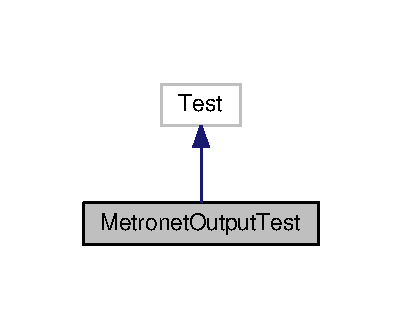
\includegraphics[width=184pt]{class_metronet_output_test__inherit__graph}
\end{center}
\end{figure}


Collaboration diagram for Metronet\+Output\+Test\+:
\nopagebreak
\begin{figure}[H]
\begin{center}
\leavevmode
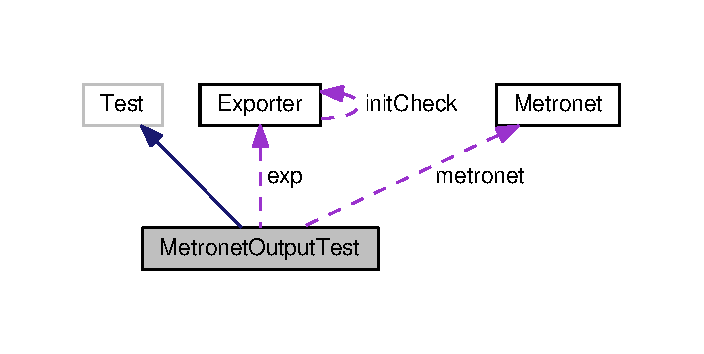
\includegraphics[width=350pt]{class_metronet_output_test__coll__graph}
\end{center}
\end{figure}
\subsection*{Protected Member Functions}
\begin{DoxyCompactItemize}
\item 
virtual void \hyperlink{class_metronet_output_test_a591685e65362fe63b325e2d33189a3b0}{Set\+Up} ()
\item 
virtual void \hyperlink{class_metronet_output_test_a1390ab64ffdb3c5da39c4b27b40c170a}{Tear\+Down} ()
\end{DoxyCompactItemize}
\subsection*{Protected Attributes}
\begin{DoxyCompactItemize}
\item 
\hyperlink{class_parser}{Parser} \hyperlink{class_metronet_output_test_a0ed101661d80432a33bb81fed2621029}{parser}
\item 
\hyperlink{class_metronet}{Metronet} \hyperlink{class_metronet_output_test_aaa6f34ee762d128cd8aea8c895bb46e4}{metronet}
\item 
\hyperlink{class_exporter}{Exporter} $\ast$ \hyperlink{class_metronet_output_test_ace0d26029b129b05d3846365c56d42ee}{exp}
\end{DoxyCompactItemize}
\subsection*{Friends}
\begin{DoxyCompactItemize}
\item 
class \hyperlink{class_metronet_output_test_a07c94fb69880743e62f64a941fc2d4ab}{Metronet}
\end{DoxyCompactItemize}


\subsection{Detailed Description}
\hyperlink{class_metronet_output_test}{Metronet\+Output\+Test} klasse die output tests behandelt. 

\subsection{Member Function Documentation}
\index{Metronet\+Output\+Test@{Metronet\+Output\+Test}!Set\+Up@{Set\+Up}}
\index{Set\+Up@{Set\+Up}!Metronet\+Output\+Test@{Metronet\+Output\+Test}}
\subsubsection[{\texorpdfstring{Set\+Up()}{SetUp()}}]{\setlength{\rightskip}{0pt plus 5cm}virtual void Metronet\+Output\+Test\+::\+Set\+Up (
\begin{DoxyParamCaption}
{}
\end{DoxyParamCaption}
)\hspace{0.3cm}{\ttfamily [inline]}, {\ttfamily [protected]}, {\ttfamily [virtual]}}\hypertarget{class_metronet_output_test_a591685e65362fe63b325e2d33189a3b0}{}\label{class_metronet_output_test_a591685e65362fe63b325e2d33189a3b0}
\index{Metronet\+Output\+Test@{Metronet\+Output\+Test}!Tear\+Down@{Tear\+Down}}
\index{Tear\+Down@{Tear\+Down}!Metronet\+Output\+Test@{Metronet\+Output\+Test}}
\subsubsection[{\texorpdfstring{Tear\+Down()}{TearDown()}}]{\setlength{\rightskip}{0pt plus 5cm}virtual void Metronet\+Output\+Test\+::\+Tear\+Down (
\begin{DoxyParamCaption}
{}
\end{DoxyParamCaption}
)\hspace{0.3cm}{\ttfamily [inline]}, {\ttfamily [protected]}, {\ttfamily [virtual]}}\hypertarget{class_metronet_output_test_a1390ab64ffdb3c5da39c4b27b40c170a}{}\label{class_metronet_output_test_a1390ab64ffdb3c5da39c4b27b40c170a}


\subsection{Friends And Related Function Documentation}
\index{Metronet\+Output\+Test@{Metronet\+Output\+Test}!Metronet@{Metronet}}
\index{Metronet@{Metronet}!Metronet\+Output\+Test@{Metronet\+Output\+Test}}
\subsubsection[{\texorpdfstring{Metronet}{Metronet}}]{\setlength{\rightskip}{0pt plus 5cm}friend class {\bf Metronet}\hspace{0.3cm}{\ttfamily [friend]}}\hypertarget{class_metronet_output_test_a07c94fb69880743e62f64a941fc2d4ab}{}\label{class_metronet_output_test_a07c94fb69880743e62f64a941fc2d4ab}


\subsection{Member Data Documentation}
\index{Metronet\+Output\+Test@{Metronet\+Output\+Test}!exp@{exp}}
\index{exp@{exp}!Metronet\+Output\+Test@{Metronet\+Output\+Test}}
\subsubsection[{\texorpdfstring{exp}{exp}}]{\setlength{\rightskip}{0pt plus 5cm}{\bf Exporter}$\ast$ Metronet\+Output\+Test\+::exp\hspace{0.3cm}{\ttfamily [protected]}}\hypertarget{class_metronet_output_test_ace0d26029b129b05d3846365c56d42ee}{}\label{class_metronet_output_test_ace0d26029b129b05d3846365c56d42ee}
\index{Metronet\+Output\+Test@{Metronet\+Output\+Test}!metronet@{metronet}}
\index{metronet@{metronet}!Metronet\+Output\+Test@{Metronet\+Output\+Test}}
\subsubsection[{\texorpdfstring{metronet}{metronet}}]{\setlength{\rightskip}{0pt plus 5cm}{\bf Metronet} Metronet\+Output\+Test\+::metronet\hspace{0.3cm}{\ttfamily [protected]}}\hypertarget{class_metronet_output_test_aaa6f34ee762d128cd8aea8c895bb46e4}{}\label{class_metronet_output_test_aaa6f34ee762d128cd8aea8c895bb46e4}
\index{Metronet\+Output\+Test@{Metronet\+Output\+Test}!parser@{parser}}
\index{parser@{parser}!Metronet\+Output\+Test@{Metronet\+Output\+Test}}
\subsubsection[{\texorpdfstring{parser}{parser}}]{\setlength{\rightskip}{0pt plus 5cm}{\bf Parser} Metronet\+Output\+Test\+::parser\hspace{0.3cm}{\ttfamily [protected]}}\hypertarget{class_metronet_output_test_a0ed101661d80432a33bb81fed2621029}{}\label{class_metronet_output_test_a0ed101661d80432a33bb81fed2621029}


The documentation for this class was generated from the following file\+:\begin{DoxyCompactItemize}
\item 
/home/jonathan/\+Desktop/\+Project Software Engineering/\+Metronet/\+P\+S\+E/src/\hyperlink{_metronet_output_test_8h}{Metronet\+Output\+Test.\+h}\end{DoxyCompactItemize}

\hypertarget{class_station}{}\section{Station Class Reference}
\label{class_station}\index{Station@{Station}}


{\ttfamily \#include $<$Station.\+h$>$}

\subsection*{Public Member Functions}
\begin{DoxyCompactItemize}
\item 
\hyperlink{class_station_a73d335726aad1d844d81cda6d9fd74e6}{Station} ()
\item 
\hyperlink{class_station_a1685ff9a628b922fbc6a75f0f23c7b7e}{Station} (std\+::string n, \hyperlink{class_station}{Station} $\ast$vor, \hyperlink{class_station}{Station} $\ast$volg, \hyperlink{class_spoor}{Spoor} $\ast$sp)
\item 
virtual \hyperlink{class_station_a00434e79e8ee7f4ebd6d3b631dde5ac0}{$\sim$\+Station} ()
\item 
bool \hyperlink{class_station_a5749af84d13b71d34aa1fb5b0a935a20}{properly\+Initialised} () const 
\begin{DoxyCompactList}\small\item\em Kijk na of de constructor in de juiste staat geeindigd is. \end{DoxyCompactList}\item 
std\+::string \hyperlink{class_station_a6d4234bcd1027dc83c7984e207e8bd74}{get\+Naam} () const 
\begin{DoxyCompactList}\small\item\em Geef de naam terug van het station. \end{DoxyCompactList}\item 
\hyperlink{class_station}{Station} $\ast$ \hyperlink{class_station_a2adced993339721e8731bfa55762f4f9}{get\+Vorige} () const 
\begin{DoxyCompactList}\small\item\em Geef het vorig station terug. \end{DoxyCompactList}\item 
\hyperlink{class_station}{Station} $\ast$ \hyperlink{class_station_a2c81d14029f13b972c015a16813c8d34}{get\+Volgende} () const 
\begin{DoxyCompactList}\small\item\em Geef het volgende station. \end{DoxyCompactList}\item 
\hyperlink{class_spoor}{Spoor} $\ast$ \hyperlink{class_station_af7ea9d2ec05b56832c0e1a2fe2303ee1}{get\+Spoor} () const 
\begin{DoxyCompactList}\small\item\em Geef het \hyperlink{class_spoor}{Spoor} terug. \end{DoxyCompactList}\end{DoxyCompactItemize}


\subsection{Constructor \& Destructor Documentation}
\index{Station@{Station}!Station@{Station}}
\index{Station@{Station}!Station@{Station}}
\subsubsection[{\texorpdfstring{Station()}{Station()}}]{\setlength{\rightskip}{0pt plus 5cm}Station\+::\+Station (
\begin{DoxyParamCaption}
{}
\end{DoxyParamCaption}
)}\hypertarget{class_station_a73d335726aad1d844d81cda6d9fd74e6}{}\label{class_station_a73d335726aad1d844d81cda6d9fd74e6}
\index{Station@{Station}!Station@{Station}}
\index{Station@{Station}!Station@{Station}}
\subsubsection[{\texorpdfstring{Station(std\+::string n, Station $\ast$vor, Station $\ast$volg, Spoor $\ast$sp)}{Station(std::string n, Station *vor, Station *volg, Spoor *sp)}}]{\setlength{\rightskip}{0pt plus 5cm}Station\+::\+Station (
\begin{DoxyParamCaption}
\item[{std\+::string}]{n, }
\item[{{\bf Station} $\ast$}]{vor, }
\item[{{\bf Station} $\ast$}]{volg, }
\item[{{\bf Spoor} $\ast$}]{sp}
\end{DoxyParamCaption}
)}\hypertarget{class_station_a1685ff9a628b922fbc6a75f0f23c7b7e}{}\label{class_station_a1685ff9a628b922fbc6a75f0f23c7b7e}
\index{Station@{Station}!````~Station@{$\sim$\+Station}}
\index{````~Station@{$\sim$\+Station}!Station@{Station}}
\subsubsection[{\texorpdfstring{$\sim$\+Station()}{~Station()}}]{\setlength{\rightskip}{0pt plus 5cm}Station\+::$\sim$\+Station (
\begin{DoxyParamCaption}
{}
\end{DoxyParamCaption}
)\hspace{0.3cm}{\ttfamily [virtual]}}\hypertarget{class_station_a00434e79e8ee7f4ebd6d3b631dde5ac0}{}\label{class_station_a00434e79e8ee7f4ebd6d3b631dde5ac0}


\subsection{Member Function Documentation}
\index{Station@{Station}!get\+Naam@{get\+Naam}}
\index{get\+Naam@{get\+Naam}!Station@{Station}}
\subsubsection[{\texorpdfstring{get\+Naam() const }{getNaam() const }}]{\setlength{\rightskip}{0pt plus 5cm}std\+::string Station\+::get\+Naam (
\begin{DoxyParamCaption}
{}
\end{DoxyParamCaption}
) const}\hypertarget{class_station_a6d4234bcd1027dc83c7984e207e8bd74}{}\label{class_station_a6d4234bcd1027dc83c7984e207e8bd74}


Geef de naam terug van het station. 

\begin{DoxyReturn}{Returns}
De naam van het station.
\end{DoxyReturn}
R\+E\+Q\+U\+I\+RE(this-\/$>$\hyperlink{class_station_a5749af84d13b71d34aa1fb5b0a935a20}{properly\+Initialised()}, \char`\"{}\+Station was niet geinitialiseerd bij de aanroep van get\+Naam.\char`\"{});~\newline


Here is the call graph for this function\+:
\nopagebreak
\begin{figure}[H]
\begin{center}
\leavevmode
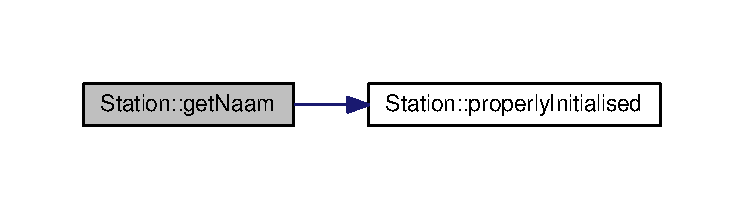
\includegraphics[width=338pt]{class_station_a6d4234bcd1027dc83c7984e207e8bd74_cgraph}
\end{center}
\end{figure}




Here is the caller graph for this function\+:
\nopagebreak
\begin{figure}[H]
\begin{center}
\leavevmode
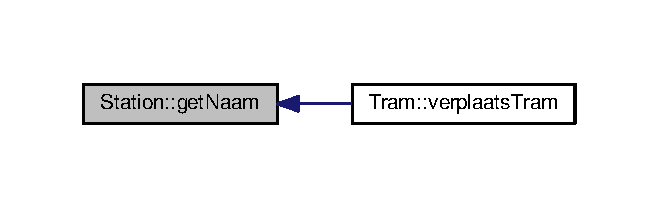
\includegraphics[width=316pt]{class_station_a6d4234bcd1027dc83c7984e207e8bd74_icgraph}
\end{center}
\end{figure}


\index{Station@{Station}!get\+Spoor@{get\+Spoor}}
\index{get\+Spoor@{get\+Spoor}!Station@{Station}}
\subsubsection[{\texorpdfstring{get\+Spoor() const }{getSpoor() const }}]{\setlength{\rightskip}{0pt plus 5cm}{\bf Spoor} $\ast$ Station\+::get\+Spoor (
\begin{DoxyParamCaption}
{}
\end{DoxyParamCaption}
) const}\hypertarget{class_station_af7ea9d2ec05b56832c0e1a2fe2303ee1}{}\label{class_station_af7ea9d2ec05b56832c0e1a2fe2303ee1}


Geef het \hyperlink{class_spoor}{Spoor} terug. 

\begin{DoxyReturn}{Returns}
Het spoor. R\+E\+Q\+U\+I\+RE(this-\/$>$\hyperlink{class_station_a5749af84d13b71d34aa1fb5b0a935a20}{properly\+Initialised()}, \char`\"{}\+Station was niet geinitialiseerd bij de aanroep van get\+Spoor.\char`\"{});~\newline

\end{DoxyReturn}


Here is the call graph for this function\+:
\nopagebreak
\begin{figure}[H]
\begin{center}
\leavevmode
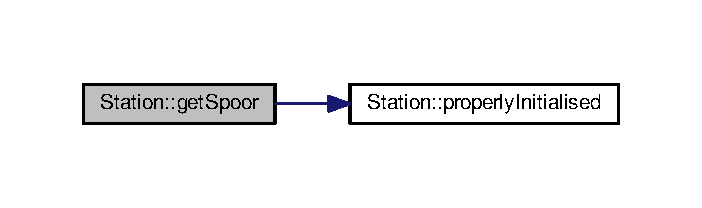
\includegraphics[width=337pt]{class_station_af7ea9d2ec05b56832c0e1a2fe2303ee1_cgraph}
\end{center}
\end{figure}


\index{Station@{Station}!get\+Volgende@{get\+Volgende}}
\index{get\+Volgende@{get\+Volgende}!Station@{Station}}
\subsubsection[{\texorpdfstring{get\+Volgende() const }{getVolgende() const }}]{\setlength{\rightskip}{0pt plus 5cm}{\bf Station} $\ast$ Station\+::get\+Volgende (
\begin{DoxyParamCaption}
{}
\end{DoxyParamCaption}
) const}\hypertarget{class_station_a2c81d14029f13b972c015a16813c8d34}{}\label{class_station_a2c81d14029f13b972c015a16813c8d34}


Geef het volgende station. 

\begin{DoxyReturn}{Returns}
Het volgende station.
\end{DoxyReturn}
R\+E\+Q\+U\+I\+RE(this-\/$>$\hyperlink{class_station_a5749af84d13b71d34aa1fb5b0a935a20}{properly\+Initialised()}, \char`\"{}\+Station was niet geinitialiseerd bij de aanroep van get\+Volgende.\char`\"{});~\newline


Here is the call graph for this function\+:
\nopagebreak
\begin{figure}[H]
\begin{center}
\leavevmode
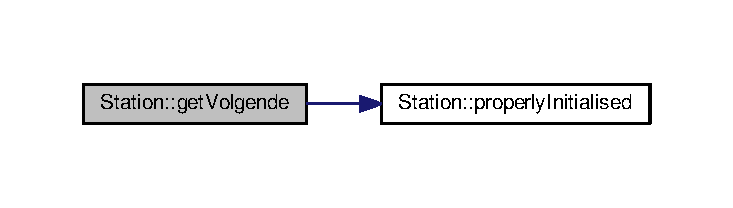
\includegraphics[width=350pt]{class_station_a2c81d14029f13b972c015a16813c8d34_cgraph}
\end{center}
\end{figure}


\index{Station@{Station}!get\+Vorige@{get\+Vorige}}
\index{get\+Vorige@{get\+Vorige}!Station@{Station}}
\subsubsection[{\texorpdfstring{get\+Vorige() const }{getVorige() const }}]{\setlength{\rightskip}{0pt plus 5cm}{\bf Station} $\ast$ Station\+::get\+Vorige (
\begin{DoxyParamCaption}
{}
\end{DoxyParamCaption}
) const}\hypertarget{class_station_a2adced993339721e8731bfa55762f4f9}{}\label{class_station_a2adced993339721e8731bfa55762f4f9}


Geef het vorig station terug. 

\begin{DoxyReturn}{Returns}
Het vorig station.
\end{DoxyReturn}
R\+E\+Q\+U\+I\+RE(this-\/$>$\hyperlink{class_station_a5749af84d13b71d34aa1fb5b0a935a20}{properly\+Initialised()}, \char`\"{}\+Station was niet geinitialiseerd bij de aanroep van get\+Vorige.\char`\"{});~\newline


Here is the call graph for this function\+:
\nopagebreak
\begin{figure}[H]
\begin{center}
\leavevmode
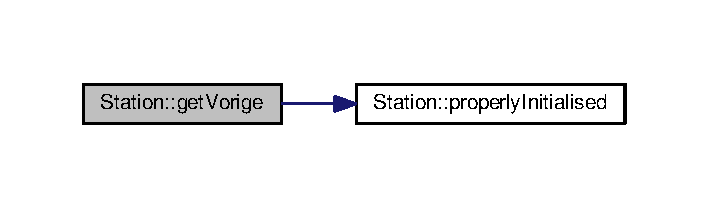
\includegraphics[width=340pt]{class_station_a2adced993339721e8731bfa55762f4f9_cgraph}
\end{center}
\end{figure}


\index{Station@{Station}!properly\+Initialised@{properly\+Initialised}}
\index{properly\+Initialised@{properly\+Initialised}!Station@{Station}}
\subsubsection[{\texorpdfstring{properly\+Initialised() const }{properlyInitialised() const }}]{\setlength{\rightskip}{0pt plus 5cm}bool Station\+::properly\+Initialised (
\begin{DoxyParamCaption}
{}
\end{DoxyParamCaption}
) const}\hypertarget{class_station_a5749af84d13b71d34aa1fb5b0a935a20}{}\label{class_station_a5749af84d13b71d34aa1fb5b0a935a20}


Kijk na of de constructor in de juiste staat geeindigd is. 

\begin{DoxyReturn}{Returns}
Boolean die aangeeft of het object juist geinitialiseerd is. 
\end{DoxyReturn}


Here is the caller graph for this function\+:
\nopagebreak
\begin{figure}[H]
\begin{center}
\leavevmode
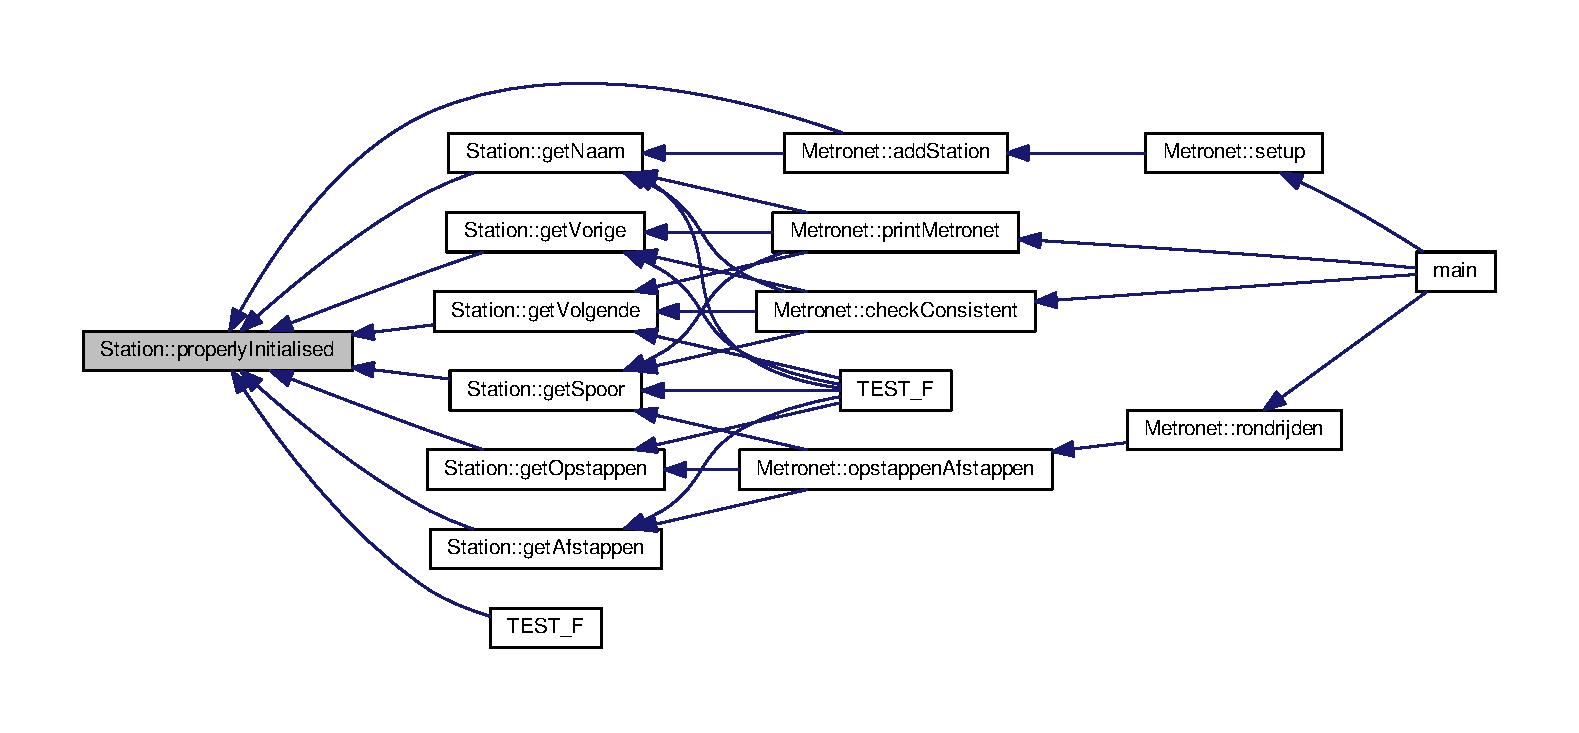
\includegraphics[width=350pt]{class_station_a5749af84d13b71d34aa1fb5b0a935a20_icgraph}
\end{center}
\end{figure}




The documentation for this class was generated from the following files\+:\begin{DoxyCompactItemize}
\item 
/home/jonathan/\+Desktop/\+Project Software Engineering/\+Metronet/\+P\+S\+E/src/\hyperlink{_station_8h}{Station.\+h}\item 
/home/jonathan/\+Desktop/\+Project Software Engineering/\+Metronet/\+P\+S\+E/src/\hyperlink{_station_8cpp}{Station.\+cpp}\end{DoxyCompactItemize}

\hypertarget{class_tram}{}\section{Tram Class Reference}
\label{class_tram}\index{Tram@{Tram}}


{\ttfamily \#include $<$Tram.\+h$>$}

\subsection*{Public Member Functions}
\begin{DoxyCompactItemize}
\item 
\hyperlink{class_tram_aad83b2e7e79d57528691bf317ab0e1ef}{Tram} ()
\item 
\hyperlink{class_tram_afef6559a85225dc0b8a9445d6d16cbbb}{Tram} (int zit, int snel, int sp, std\+::string beginS)
\item 
bool \hyperlink{class_tram_a98992eff0453f54fbe64e1f1064169c7}{properly\+Initialised} () const 
\begin{DoxyCompactList}\small\item\em Kijk na of de constructor in de juiste staat geeindigd is. \end{DoxyCompactList}\item 
int \hyperlink{class_tram_aa366e37291186d6cfd402aa7b6cfec2d}{get\+Zitplaatsen} () const 
\begin{DoxyCompactList}\small\item\em Geef de zitplaatsen terug van de tram. \end{DoxyCompactList}\item 
int \hyperlink{class_tram_a8e9e449f0032f0f439c196e0980a891e}{get\+Passagiers} () const 
\begin{DoxyCompactList}\small\item\em Geef de passagiers terug van de tram. \end{DoxyCompactList}\item 
int \hyperlink{class_tram_a40a12ae66cdc8965fc73d548dd038e4c}{get\+Snelheid} () const 
\begin{DoxyCompactList}\small\item\em Geef de snelheid terug van de tram. \end{DoxyCompactList}\item 
int \hyperlink{class_tram_a52655f991ffb58a8ab3557fd881a6f58}{get\+Spoor} () const 
\begin{DoxyCompactList}\small\item\em Geef het spoor terug. \end{DoxyCompactList}\item 
std\+::string \hyperlink{class_tram_aba7b84414cd60d013ac1db3f3403497d}{get\+Begin\+Station} () const 
\begin{DoxyCompactList}\small\item\em Geef het beginstation terug. \end{DoxyCompactList}\item 
std\+::string \hyperlink{class_tram_ae7bc337a42b2d839b4da5f648b781e79}{get\+Huidig\+Station} () const 
\begin{DoxyCompactList}\small\item\em Geef het huidig station. \end{DoxyCompactList}\item 
void \hyperlink{class_tram_a8d55296c7ede4aa92c9b3a4b2a9495a8}{verplaats\+Tram} (std\+::string station, \hyperlink{class_exporter}{Exporter} $\ast$exp, std\+::ostream \&os)
\begin{DoxyCompactList}\small\item\em Verplaatst een tram naar het opgegeven station. \end{DoxyCompactList}\item 
bool \hyperlink{class_tram_a81186910caa5212b4a87eec84cd10a46}{afstappen} (int afstappen)
\begin{DoxyCompactList}\small\item\em Emuleert afstappen van passagiers. (Nieuw huidig aantal = huidig aantal -\/ afstappende passagiers) \end{DoxyCompactList}\item 
bool \hyperlink{class_tram_aaeb00c535a6854f85dcc42cdff97ad0c}{opstappen} (int opstappen)
\begin{DoxyCompactList}\small\item\em Emuleert opstappen van passagiers. (Nieuw huidig aantal = huidig aantal + opstappende passagiers) \end{DoxyCompactList}\end{DoxyCompactItemize}


\subsection{Constructor \& Destructor Documentation}
\index{Tram@{Tram}!Tram@{Tram}}
\index{Tram@{Tram}!Tram@{Tram}}
\subsubsection[{\texorpdfstring{Tram()}{Tram()}}]{\setlength{\rightskip}{0pt plus 5cm}Tram\+::\+Tram (
\begin{DoxyParamCaption}
{}
\end{DoxyParamCaption}
)}\hypertarget{class_tram_aad83b2e7e79d57528691bf317ab0e1ef}{}\label{class_tram_aad83b2e7e79d57528691bf317ab0e1ef}
\index{Tram@{Tram}!Tram@{Tram}}
\index{Tram@{Tram}!Tram@{Tram}}
\subsubsection[{\texorpdfstring{Tram(int zit, int snel, int sp, std\+::string begin\+S)}{Tram(int zit, int snel, int sp, std::string beginS)}}]{\setlength{\rightskip}{0pt plus 5cm}Tram\+::\+Tram (
\begin{DoxyParamCaption}
\item[{int}]{zit, }
\item[{int}]{snel, }
\item[{int}]{sp, }
\item[{std\+::string}]{beginS}
\end{DoxyParamCaption}
)}\hypertarget{class_tram_afef6559a85225dc0b8a9445d6d16cbbb}{}\label{class_tram_afef6559a85225dc0b8a9445d6d16cbbb}


\subsection{Member Function Documentation}
\index{Tram@{Tram}!afstappen@{afstappen}}
\index{afstappen@{afstappen}!Tram@{Tram}}
\subsubsection[{\texorpdfstring{afstappen(int afstappen)}{afstappen(int afstappen)}}]{\setlength{\rightskip}{0pt plus 5cm}bool Tram\+::afstappen (
\begin{DoxyParamCaption}
\item[{int}]{afstappen}
\end{DoxyParamCaption}
)}\hypertarget{class_tram_a81186910caa5212b4a87eec84cd10a46}{}\label{class_tram_a81186910caa5212b4a87eec84cd10a46}


Emuleert afstappen van passagiers. (Nieuw huidig aantal = huidig aantal -\/ afstappende passagiers) 


\begin{DoxyParams}{Parameters}
{\em afstappen} & Aantal passagiers dat afstapt. \\
\hline
\end{DoxyParams}
\begin{DoxyReturn}{Returns}
boolean Of er meer passagiers afstapten dan mogelijk.
\end{DoxyReturn}
R\+E\+Q\+U\+I\+RE(this-\/$>$\hyperlink{class_tram_a98992eff0453f54fbe64e1f1064169c7}{properly\+Initialised()}, \char`\"{}\+Tram was niet geinitialiseerd bij de aanroep van afstappen.\char`\"{});~\newline


Here is the call graph for this function\+:
\nopagebreak
\begin{figure}[H]
\begin{center}
\leavevmode
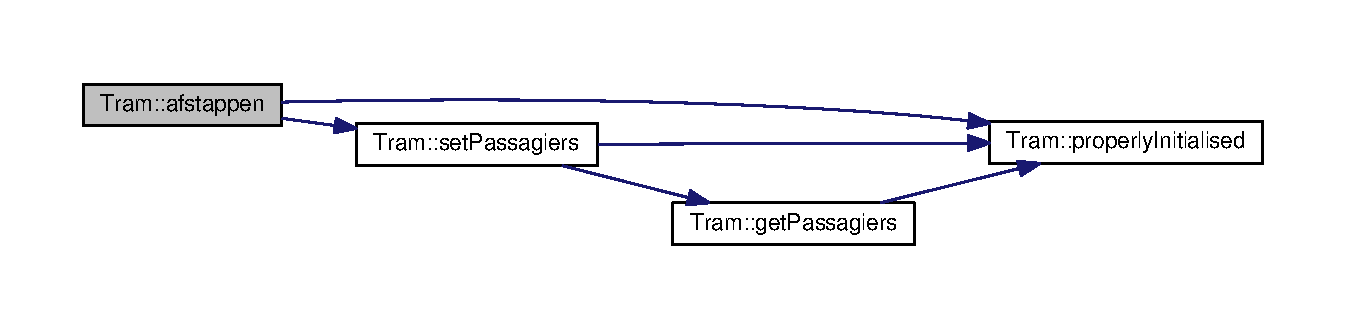
\includegraphics[width=325pt]{class_tram_a81186910caa5212b4a87eec84cd10a46_cgraph}
\end{center}
\end{figure}




Here is the caller graph for this function\+:
\nopagebreak
\begin{figure}[H]
\begin{center}
\leavevmode
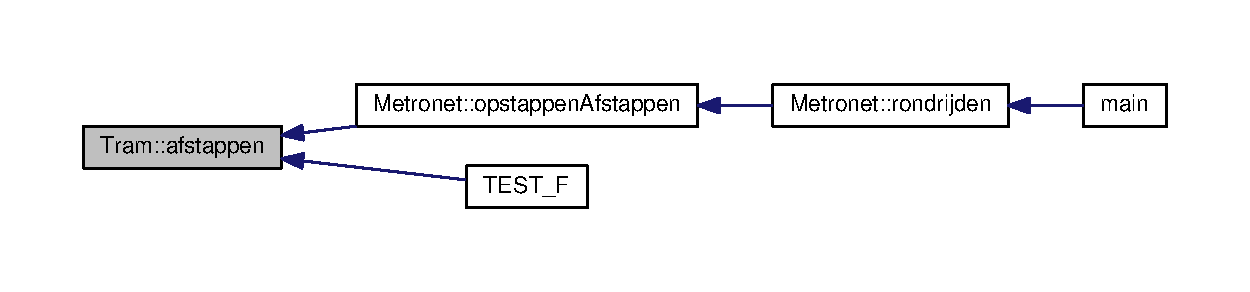
\includegraphics[width=350pt]{class_tram_a81186910caa5212b4a87eec84cd10a46_icgraph}
\end{center}
\end{figure}


\index{Tram@{Tram}!get\+Begin\+Station@{get\+Begin\+Station}}
\index{get\+Begin\+Station@{get\+Begin\+Station}!Tram@{Tram}}
\subsubsection[{\texorpdfstring{get\+Begin\+Station() const }{getBeginStation() const }}]{\setlength{\rightskip}{0pt plus 5cm}std\+::string Tram\+::get\+Begin\+Station (
\begin{DoxyParamCaption}
{}
\end{DoxyParamCaption}
) const}\hypertarget{class_tram_aba7b84414cd60d013ac1db3f3403497d}{}\label{class_tram_aba7b84414cd60d013ac1db3f3403497d}


Geef het beginstation terug. 

\begin{DoxyReturn}{Returns}
Het beginstation.
\end{DoxyReturn}
R\+E\+Q\+U\+I\+RE(this-\/$>$\hyperlink{class_tram_a98992eff0453f54fbe64e1f1064169c7}{properly\+Initialised()}, \char`\"{}\+Tram was niet geinitialiseerd bij de aanroep van get\+Begin\+Station.\char`\"{});~\newline


Here is the call graph for this function\+:
\nopagebreak
\begin{figure}[H]
\begin{center}
\leavevmode
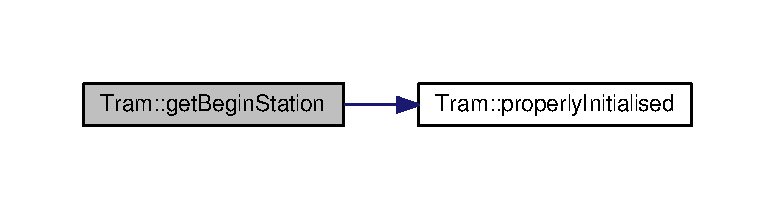
\includegraphics[width=350pt]{class_tram_aba7b84414cd60d013ac1db3f3403497d_cgraph}
\end{center}
\end{figure}




Here is the caller graph for this function\+:
\nopagebreak
\begin{figure}[H]
\begin{center}
\leavevmode
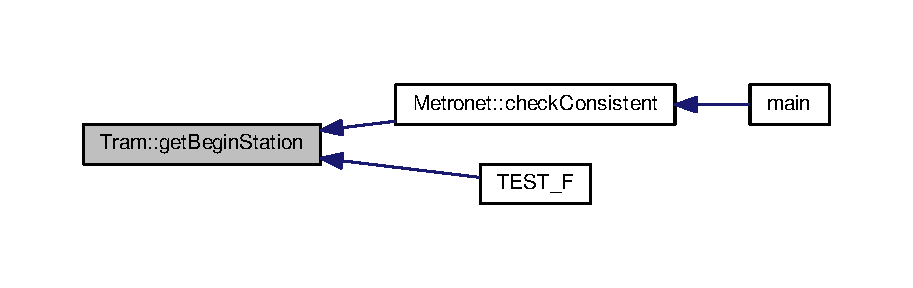
\includegraphics[width=350pt]{class_tram_aba7b84414cd60d013ac1db3f3403497d_icgraph}
\end{center}
\end{figure}


\index{Tram@{Tram}!get\+Huidig\+Station@{get\+Huidig\+Station}}
\index{get\+Huidig\+Station@{get\+Huidig\+Station}!Tram@{Tram}}
\subsubsection[{\texorpdfstring{get\+Huidig\+Station() const }{getHuidigStation() const }}]{\setlength{\rightskip}{0pt plus 5cm}std\+::string Tram\+::get\+Huidig\+Station (
\begin{DoxyParamCaption}
{}
\end{DoxyParamCaption}
) const}\hypertarget{class_tram_ae7bc337a42b2d839b4da5f648b781e79}{}\label{class_tram_ae7bc337a42b2d839b4da5f648b781e79}


Geef het huidig station. 

\begin{DoxyReturn}{Returns}
Het huidig station.
\end{DoxyReturn}
R\+E\+Q\+U\+I\+RE(this-\/$>$\hyperlink{class_tram_a98992eff0453f54fbe64e1f1064169c7}{properly\+Initialised()}, \char`\"{}\+Tram was niet geinitialiseerd bij de aanroep van get\+Huidig\+Station.\char`\"{});~\newline


Here is the call graph for this function\+:
\nopagebreak
\begin{figure}[H]
\begin{center}
\leavevmode
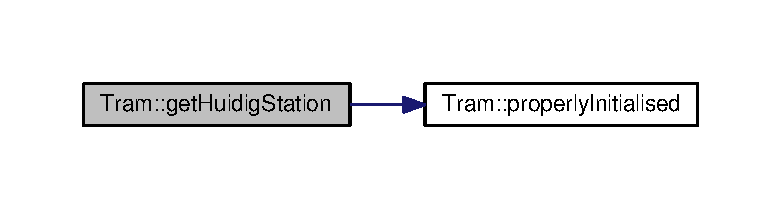
\includegraphics[width=350pt]{class_tram_ae7bc337a42b2d839b4da5f648b781e79_cgraph}
\end{center}
\end{figure}




Here is the caller graph for this function\+:
\nopagebreak
\begin{figure}[H]
\begin{center}
\leavevmode
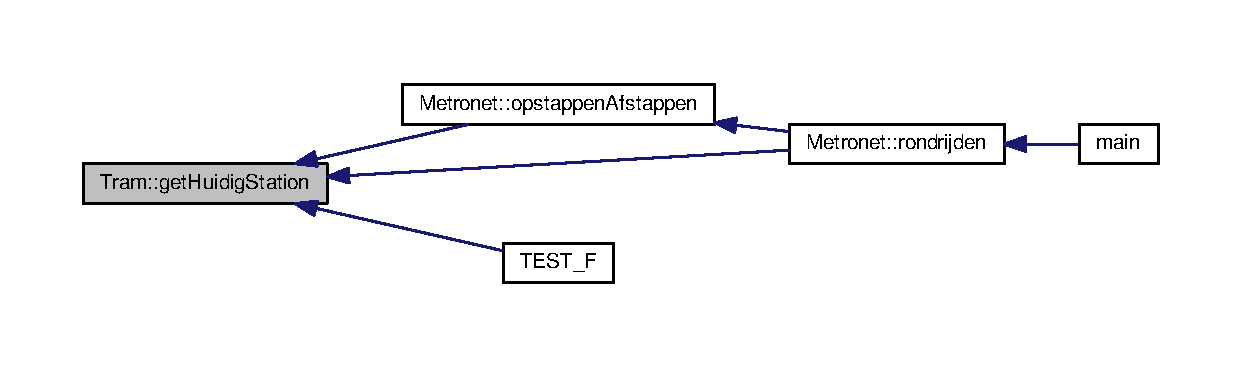
\includegraphics[width=350pt]{class_tram_ae7bc337a42b2d839b4da5f648b781e79_icgraph}
\end{center}
\end{figure}


\index{Tram@{Tram}!get\+Passagiers@{get\+Passagiers}}
\index{get\+Passagiers@{get\+Passagiers}!Tram@{Tram}}
\subsubsection[{\texorpdfstring{get\+Passagiers() const }{getPassagiers() const }}]{\setlength{\rightskip}{0pt plus 5cm}int Tram\+::get\+Passagiers (
\begin{DoxyParamCaption}
{}
\end{DoxyParamCaption}
) const}\hypertarget{class_tram_a8e9e449f0032f0f439c196e0980a891e}{}\label{class_tram_a8e9e449f0032f0f439c196e0980a891e}


Geef de passagiers terug van de tram. 

\begin{DoxyReturn}{Returns}
De passagiers.
\end{DoxyReturn}
R\+E\+Q\+U\+I\+RE(this-\/$>$\hyperlink{class_tram_a98992eff0453f54fbe64e1f1064169c7}{properly\+Initialised()}, \char`\"{}\+Tram was niet geinitialiseerd bij de aanroep van get\+Passagiers.\char`\"{});~\newline


Here is the call graph for this function\+:\nopagebreak
\begin{figure}[H]
\begin{center}
\leavevmode
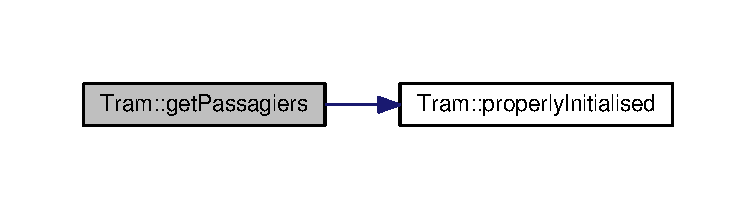
\includegraphics[width=344pt]{class_tram_a8e9e449f0032f0f439c196e0980a891e_cgraph}
\end{center}
\end{figure}


\index{Tram@{Tram}!get\+Snelheid@{get\+Snelheid}}
\index{get\+Snelheid@{get\+Snelheid}!Tram@{Tram}}
\subsubsection[{\texorpdfstring{get\+Snelheid() const }{getSnelheid() const }}]{\setlength{\rightskip}{0pt plus 5cm}int Tram\+::get\+Snelheid (
\begin{DoxyParamCaption}
{}
\end{DoxyParamCaption}
) const}\hypertarget{class_tram_a40a12ae66cdc8965fc73d548dd038e4c}{}\label{class_tram_a40a12ae66cdc8965fc73d548dd038e4c}


Geef de snelheid terug van de tram. 

\begin{DoxyReturn}{Returns}
De snelheid.
\end{DoxyReturn}
R\+E\+Q\+U\+I\+RE(this-\/$>$\hyperlink{class_tram_a98992eff0453f54fbe64e1f1064169c7}{properly\+Initialised()}, \char`\"{}\+Tram was niet geinitialiseerd bij de aanroep van get\+Snelheid.\char`\"{});~\newline


Here is the call graph for this function\+:\nopagebreak
\begin{figure}[H]
\begin{center}
\leavevmode
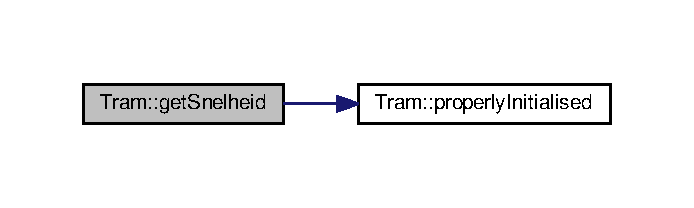
\includegraphics[width=333pt]{class_tram_a40a12ae66cdc8965fc73d548dd038e4c_cgraph}
\end{center}
\end{figure}


\index{Tram@{Tram}!get\+Spoor@{get\+Spoor}}
\index{get\+Spoor@{get\+Spoor}!Tram@{Tram}}
\subsubsection[{\texorpdfstring{get\+Spoor() const }{getSpoor() const }}]{\setlength{\rightskip}{0pt plus 5cm}int Tram\+::get\+Spoor (
\begin{DoxyParamCaption}
{}
\end{DoxyParamCaption}
) const}\hypertarget{class_tram_a52655f991ffb58a8ab3557fd881a6f58}{}\label{class_tram_a52655f991ffb58a8ab3557fd881a6f58}


Geef het spoor terug. 

\begin{DoxyReturn}{Returns}
Het spoor.
\end{DoxyReturn}
R\+E\+Q\+U\+I\+RE(this-\/$>$\hyperlink{class_tram_a98992eff0453f54fbe64e1f1064169c7}{properly\+Initialised()}, \char`\"{}\+Tram was niet geinitialiseerd bij de aanroep van get\+Spoor.\char`\"{});~\newline


Here is the call graph for this function\+:
\nopagebreak
\begin{figure}[H]
\begin{center}
\leavevmode
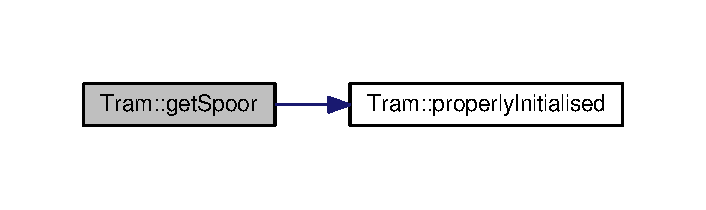
\includegraphics[width=321pt]{class_tram_a52655f991ffb58a8ab3557fd881a6f58_cgraph}
\end{center}
\end{figure}




Here is the caller graph for this function\+:
\nopagebreak
\begin{figure}[H]
\begin{center}
\leavevmode
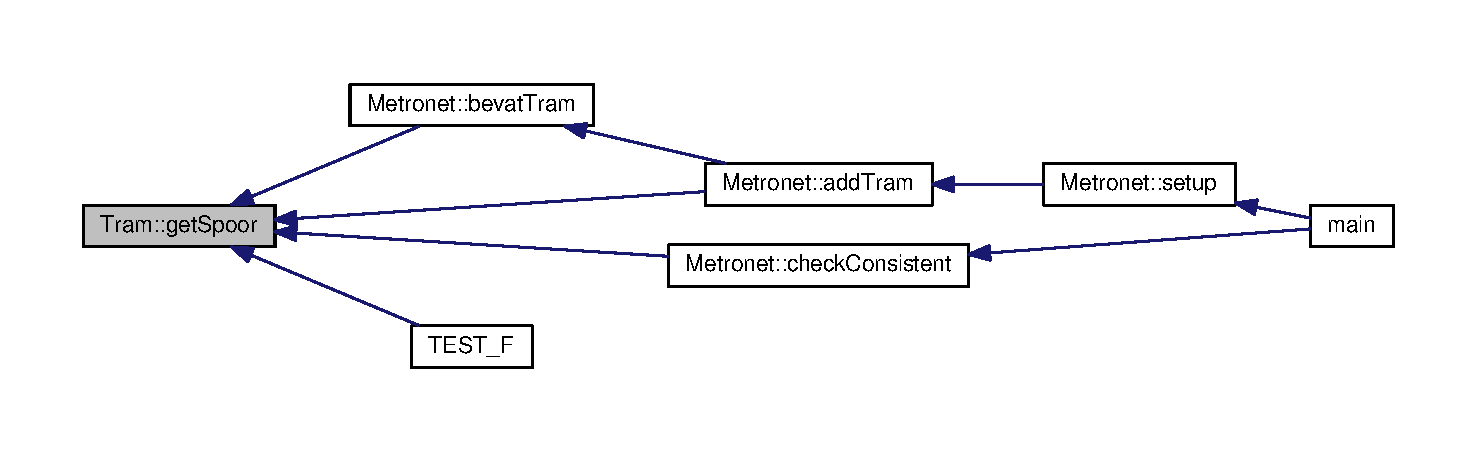
\includegraphics[width=350pt]{class_tram_a52655f991ffb58a8ab3557fd881a6f58_icgraph}
\end{center}
\end{figure}


\index{Tram@{Tram}!get\+Zitplaatsen@{get\+Zitplaatsen}}
\index{get\+Zitplaatsen@{get\+Zitplaatsen}!Tram@{Tram}}
\subsubsection[{\texorpdfstring{get\+Zitplaatsen() const }{getZitplaatsen() const }}]{\setlength{\rightskip}{0pt plus 5cm}int Tram\+::get\+Zitplaatsen (
\begin{DoxyParamCaption}
{}
\end{DoxyParamCaption}
) const}\hypertarget{class_tram_aa366e37291186d6cfd402aa7b6cfec2d}{}\label{class_tram_aa366e37291186d6cfd402aa7b6cfec2d}


Geef de zitplaatsen terug van de tram. 

\begin{DoxyReturn}{Returns}
De zitplaatsen.
\end{DoxyReturn}
R\+E\+Q\+U\+I\+RE(this-\/$>$\hyperlink{class_tram_a98992eff0453f54fbe64e1f1064169c7}{properly\+Initialised()}, \char`\"{}\+Tram was niet geinitialiseerd bij de aanroep van get\+Zitplaatsen.\char`\"{});~\newline


Here is the call graph for this function\+:\nopagebreak
\begin{figure}[H]
\begin{center}
\leavevmode
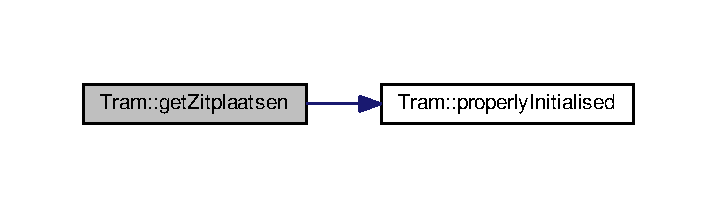
\includegraphics[width=344pt]{class_tram_aa366e37291186d6cfd402aa7b6cfec2d_cgraph}
\end{center}
\end{figure}


\index{Tram@{Tram}!opstappen@{opstappen}}
\index{opstappen@{opstappen}!Tram@{Tram}}
\subsubsection[{\texorpdfstring{opstappen(int opstappen)}{opstappen(int opstappen)}}]{\setlength{\rightskip}{0pt plus 5cm}bool Tram\+::opstappen (
\begin{DoxyParamCaption}
\item[{int}]{opstappen}
\end{DoxyParamCaption}
)}\hypertarget{class_tram_aaeb00c535a6854f85dcc42cdff97ad0c}{}\label{class_tram_aaeb00c535a6854f85dcc42cdff97ad0c}


Emuleert opstappen van passagiers. (Nieuw huidig aantal = huidig aantal + opstappende passagiers) 


\begin{DoxyParams}{Parameters}
{\em opstappen} & Aantal passagiers dat opstapt. \\
\hline
\end{DoxyParams}
\begin{DoxyReturn}{Returns}
boolean Of er meer passigiers opstapten dan mogelijk.
\end{DoxyReturn}
R\+E\+Q\+U\+I\+RE(this-\/$>$\hyperlink{class_tram_a98992eff0453f54fbe64e1f1064169c7}{properly\+Initialised()}, \char`\"{}\+Tram was niet geinitialiseerd bij de aanroep van opstappen.\char`\"{});~\newline


Here is the call graph for this function\+:
\nopagebreak
\begin{figure}[H]
\begin{center}
\leavevmode
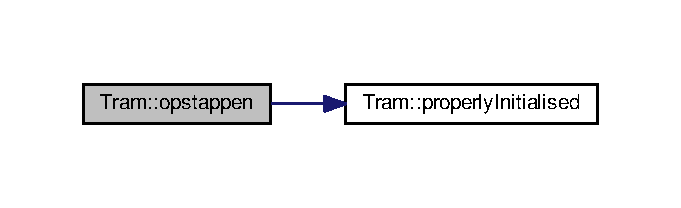
\includegraphics[width=327pt]{class_tram_aaeb00c535a6854f85dcc42cdff97ad0c_cgraph}
\end{center}
\end{figure}




Here is the caller graph for this function\+:
\nopagebreak
\begin{figure}[H]
\begin{center}
\leavevmode
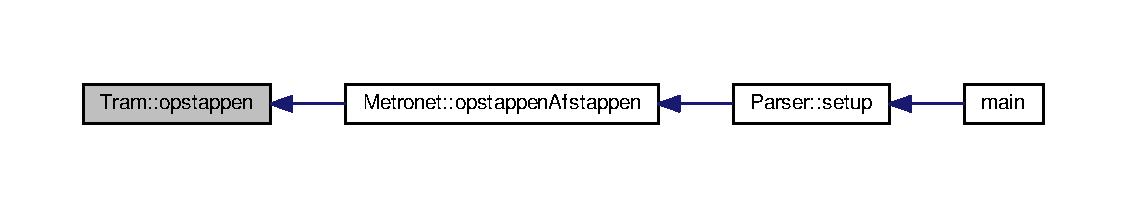
\includegraphics[width=350pt]{class_tram_aaeb00c535a6854f85dcc42cdff97ad0c_icgraph}
\end{center}
\end{figure}


\index{Tram@{Tram}!properly\+Initialised@{properly\+Initialised}}
\index{properly\+Initialised@{properly\+Initialised}!Tram@{Tram}}
\subsubsection[{\texorpdfstring{properly\+Initialised() const }{properlyInitialised() const }}]{\setlength{\rightskip}{0pt plus 5cm}bool Tram\+::properly\+Initialised (
\begin{DoxyParamCaption}
{}
\end{DoxyParamCaption}
) const}\hypertarget{class_tram_a98992eff0453f54fbe64e1f1064169c7}{}\label{class_tram_a98992eff0453f54fbe64e1f1064169c7}


Kijk na of de constructor in de juiste staat geeindigd is. 

\begin{DoxyReturn}{Returns}
Boolean die aangeeft of het object juist geinitialiseerd is. 
\end{DoxyReturn}


Here is the caller graph for this function\+:
\nopagebreak
\begin{figure}[H]
\begin{center}
\leavevmode
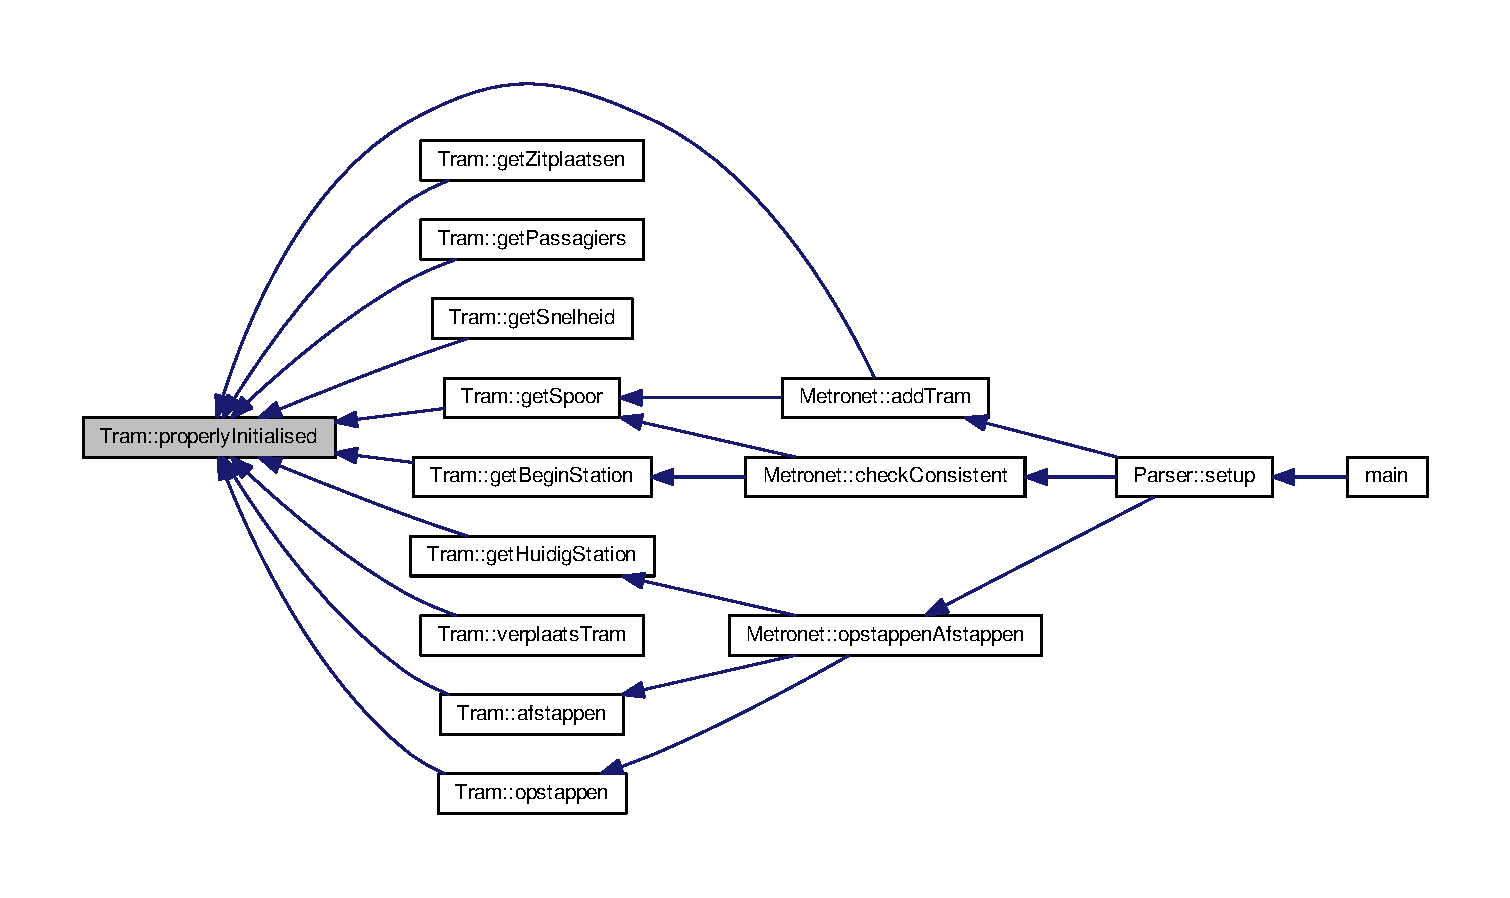
\includegraphics[width=350pt]{class_tram_a98992eff0453f54fbe64e1f1064169c7_icgraph}
\end{center}
\end{figure}


\index{Tram@{Tram}!verplaats\+Tram@{verplaats\+Tram}}
\index{verplaats\+Tram@{verplaats\+Tram}!Tram@{Tram}}
\subsubsection[{\texorpdfstring{verplaats\+Tram(std\+::string station, Exporter $\ast$exp, std\+::ostream \&os)}{verplaatsTram(std::string station, Exporter *exp, std::ostream &os)}}]{\setlength{\rightskip}{0pt plus 5cm}void Tram\+::verplaats\+Tram (
\begin{DoxyParamCaption}
\item[{std\+::string}]{station, }
\item[{{\bf Exporter} $\ast$}]{exp, }
\item[{std\+::ostream \&}]{os}
\end{DoxyParamCaption}
)}\hypertarget{class_tram_a8d55296c7ede4aa92c9b3a4b2a9495a8}{}\label{class_tram_a8d55296c7ede4aa92c9b3a4b2a9495a8}


Verplaatst een tram naar het opgegeven station. 

R\+E\+Q\+U\+I\+RE(this-\/$>$\hyperlink{class_tram_a98992eff0453f54fbe64e1f1064169c7}{properly\+Initialised()}, \char`\"{}\+Tram was niet geinitialiseerd bij de aanroep van verplaats\+Tram.\char`\"{});~\newline
E\+N\+S\+U\+RE((huidig\+Station == station), \char`\"{}huidig\+Station is niet correct aangepast.\char`\"{});~\newline


Here is the call graph for this function\+:
\nopagebreak
\begin{figure}[H]
\begin{center}
\leavevmode
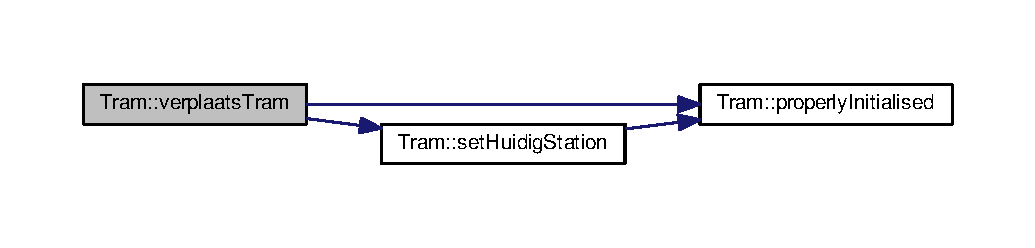
\includegraphics[width=344pt]{class_tram_a8d55296c7ede4aa92c9b3a4b2a9495a8_cgraph}
\end{center}
\end{figure}




The documentation for this class was generated from the following files\+:\begin{DoxyCompactItemize}
\item 
/home/jonathan/\+Desktop/\+Project Software Engineering/\+Metronet/\+P\+S\+E/src/\hyperlink{_tram_8h}{Tram.\+h}\item 
/home/jonathan/\+Desktop/\+Project Software Engineering/\+Metronet/\+P\+S\+E/src/\hyperlink{_tram_8cpp}{Tram.\+cpp}\end{DoxyCompactItemize}

\chapter{File Documentation}
\hypertarget{_design_by_contract_8h}{}\section{/home/sergio/\+C\+Lion\+Projects/\+Soft\+Eng/src/\+Design\+By\+Contract.h File Reference}
\label{_design_by_contract_8h}\index{/home/sergio/\+C\+Lion\+Projects/\+Soft\+Eng/src/\+Design\+By\+Contract.\+h@{/home/sergio/\+C\+Lion\+Projects/\+Soft\+Eng/src/\+Design\+By\+Contract.\+h}}
{\ttfamily \#include $<$assert.\+h$>$}\newline
Include dependency graph for Design\+By\+Contract.\+h\+:\nopagebreak
\begin{figure}[H]
\begin{center}
\leavevmode
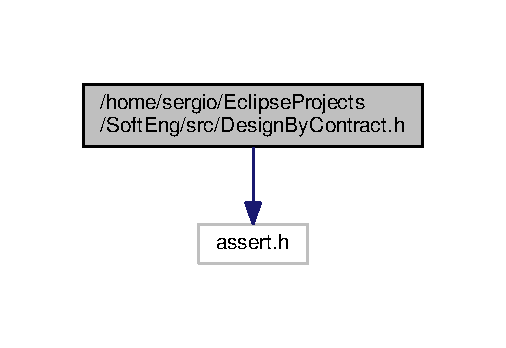
\includegraphics[width=243pt]{_design_by_contract_8h__incl}
\end{center}
\end{figure}
This graph shows which files directly or indirectly include this file\+:\nopagebreak
\begin{figure}[H]
\begin{center}
\leavevmode
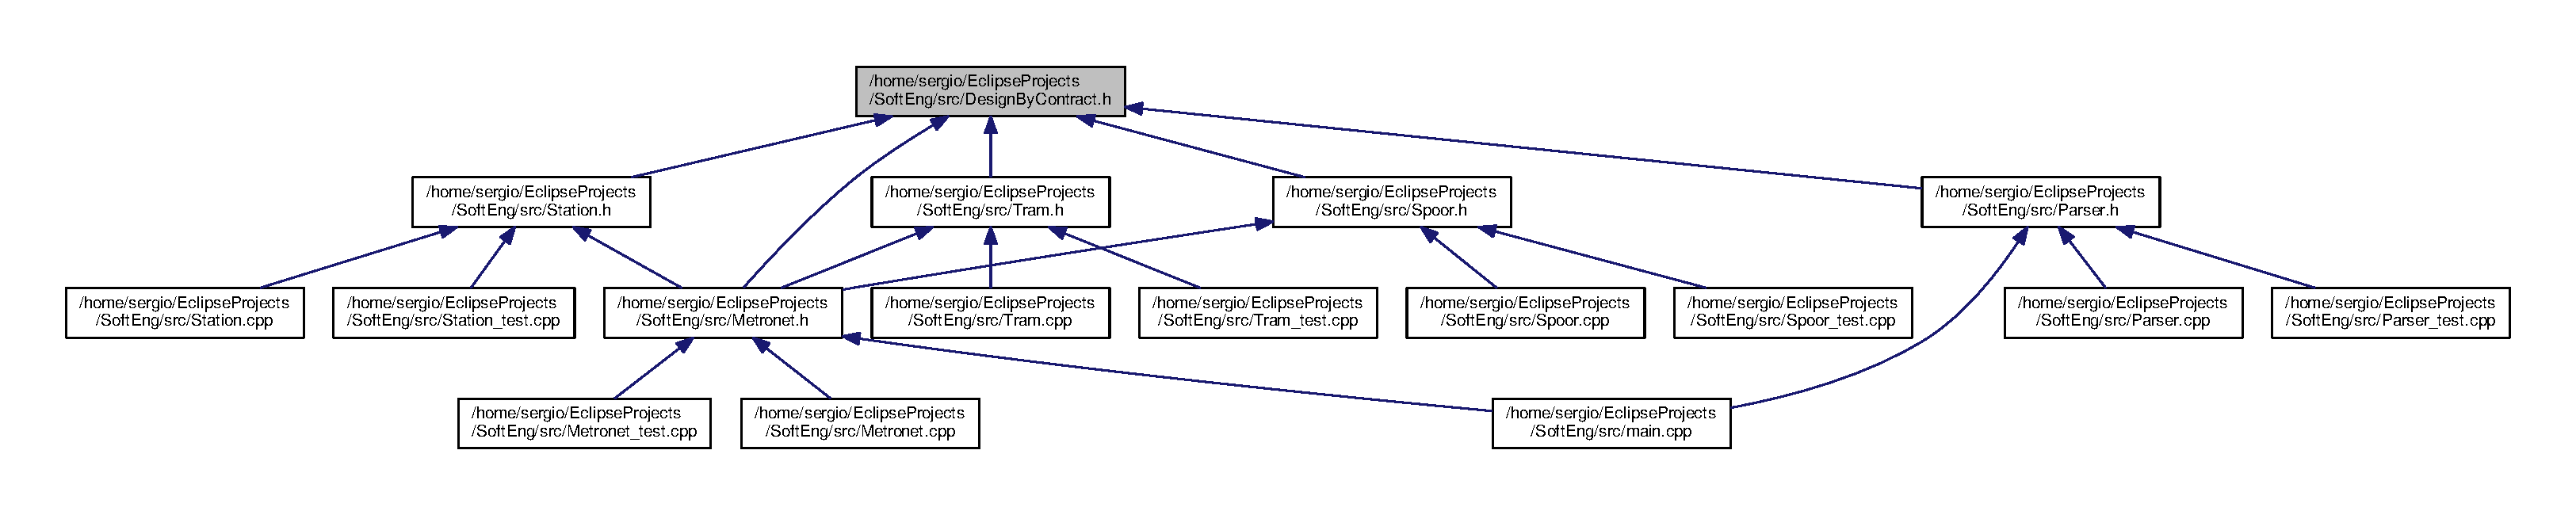
\includegraphics[width=350pt]{_design_by_contract_8h__dep__incl}
\end{center}
\end{figure}
\subsection*{Macros}
\begin{DoxyCompactItemize}
\item 
\#define \hyperlink{_design_by_contract_8h_aeb774672b46dbe80afc14e0d1970f017}{R\+E\+Q\+U\+I\+RE}(assertion,  what)~if (!(assertion)) \+\_\+\+\_\+assert (what, \+\_\+\+\_\+\+F\+I\+L\+E\+\_\+\+\_\+, \+\_\+\+\_\+\+L\+I\+N\+E\+\_\+\+\_\+)
\item 
\#define \hyperlink{_design_by_contract_8h_ab8da60ea2bcdd55183cc29d8526e6857}{E\+N\+S\+U\+RE}(assertion,  what)~if (!(assertion)) \+\_\+\+\_\+assert (what, \+\_\+\+\_\+\+F\+I\+L\+E\+\_\+\+\_\+, \+\_\+\+\_\+\+L\+I\+N\+E\+\_\+\+\_\+)
\end{DoxyCompactItemize}


\subsection{Macro Definition Documentation}
\mbox{\Hypertarget{_design_by_contract_8h_ab8da60ea2bcdd55183cc29d8526e6857}\label{_design_by_contract_8h_ab8da60ea2bcdd55183cc29d8526e6857}} 
\index{Design\+By\+Contract.\+h@{Design\+By\+Contract.\+h}!E\+N\+S\+U\+RE@{E\+N\+S\+U\+RE}}
\index{E\+N\+S\+U\+RE@{E\+N\+S\+U\+RE}!Design\+By\+Contract.\+h@{Design\+By\+Contract.\+h}}
\subsubsection{\texorpdfstring{E\+N\+S\+U\+RE}{ENSURE}}
{\footnotesize\ttfamily \#define E\+N\+S\+U\+RE(\begin{DoxyParamCaption}\item[{}]{assertion,  }\item[{}]{what }\end{DoxyParamCaption})~if (!(assertion)) \+\_\+\+\_\+assert (what, \+\_\+\+\_\+\+F\+I\+L\+E\+\_\+\+\_\+, \+\_\+\+\_\+\+L\+I\+N\+E\+\_\+\+\_\+)}

\mbox{\Hypertarget{_design_by_contract_8h_aeb774672b46dbe80afc14e0d1970f017}\label{_design_by_contract_8h_aeb774672b46dbe80afc14e0d1970f017}} 
\index{Design\+By\+Contract.\+h@{Design\+By\+Contract.\+h}!R\+E\+Q\+U\+I\+RE@{R\+E\+Q\+U\+I\+RE}}
\index{R\+E\+Q\+U\+I\+RE@{R\+E\+Q\+U\+I\+RE}!Design\+By\+Contract.\+h@{Design\+By\+Contract.\+h}}
\subsubsection{\texorpdfstring{R\+E\+Q\+U\+I\+RE}{REQUIRE}}
{\footnotesize\ttfamily \#define R\+E\+Q\+U\+I\+RE(\begin{DoxyParamCaption}\item[{}]{assertion,  }\item[{}]{what }\end{DoxyParamCaption})~if (!(assertion)) \+\_\+\+\_\+assert (what, \+\_\+\+\_\+\+F\+I\+L\+E\+\_\+\+\_\+, \+\_\+\+\_\+\+L\+I\+N\+E\+\_\+\+\_\+)}


\hypertarget{_exporter_8cpp}{}\section{/home/jonathan/\+Desktop/\+Project Software Engineering/\+Metronet/\+P\+S\+E/src/\+Exporter.cpp File Reference}
\label{_exporter_8cpp}\index{/home/jonathan/\+Desktop/\+Project Software Engineering/\+Metronet/\+P\+S\+E/src/\+Exporter.\+cpp@{/home/jonathan/\+Desktop/\+Project Software Engineering/\+Metronet/\+P\+S\+E/src/\+Exporter.\+cpp}}
{\ttfamily \#include \char`\"{}Exporter.\+h\char`\"{}}\\*
Include dependency graph for Exporter.\+cpp\+:
\nopagebreak
\begin{figure}[H]
\begin{center}
\leavevmode
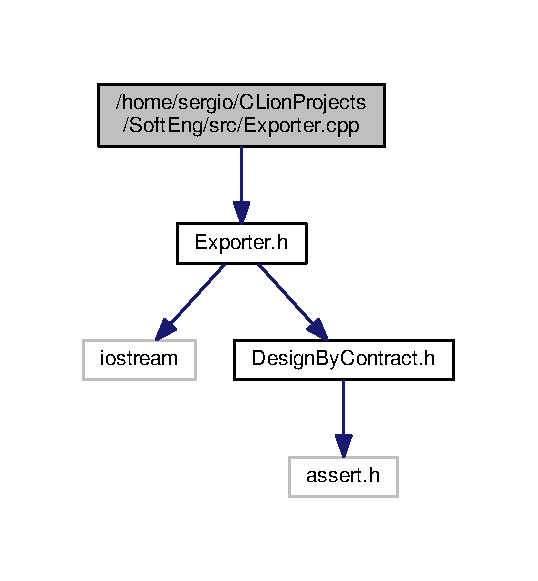
\includegraphics[width=260pt]{_exporter_8cpp__incl}
\end{center}
\end{figure}

\hypertarget{_exporter_8h}{}\section{/home/sergio/\+C\+Lion\+Projects/\+Soft\+Eng/src/\+Exporter.h File Reference}
\label{_exporter_8h}\index{/home/sergio/\+C\+Lion\+Projects/\+Soft\+Eng/src/\+Exporter.\+h@{/home/sergio/\+C\+Lion\+Projects/\+Soft\+Eng/src/\+Exporter.\+h}}
{\ttfamily \#include $<$iostream$>$}\newline
{\ttfamily \#include \char`\"{}Design\+By\+Contract.\+h\char`\"{}}\newline
Include dependency graph for Exporter.\+h\+:
\nopagebreak
\begin{figure}[H]
\begin{center}
\leavevmode
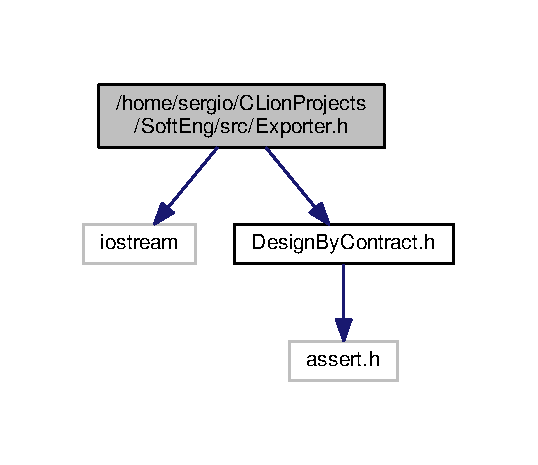
\includegraphics[width=258pt]{_exporter_8h__incl}
\end{center}
\end{figure}
This graph shows which files directly or indirectly include this file\+:
\nopagebreak
\begin{figure}[H]
\begin{center}
\leavevmode
\includegraphics[width=350pt]{_exporter_8h__dep__incl}
\end{center}
\end{figure}
\subsection*{Classes}
\begin{DoxyCompactItemize}
\item 
class \hyperlink{class_exporter}{Exporter}
\item 
class \hyperlink{class_exporter_c_l_i}{Exporter\+C\+LI}
\item 
class \hyperlink{class_exporter_t_x_t}{Exporter\+T\+XT}
\item 
class \hyperlink{class_exporter_h_t_m_l}{Exporter\+H\+T\+ML}
\end{DoxyCompactItemize}

\hypertarget{main_8cpp}{}\section{/home/sergio/\+Eclipse\+Projects/\+Soft\+Eng/src/main.cpp File Reference}
\label{main_8cpp}\index{/home/sergio/\+Eclipse\+Projects/\+Soft\+Eng/src/main.\+cpp@{/home/sergio/\+Eclipse\+Projects/\+Soft\+Eng/src/main.\+cpp}}
{\ttfamily \#include $<$iostream$>$}\newline
{\ttfamily \#include \char`\"{}Metronet.\+h\char`\"{}}\newline
{\ttfamily \#include \char`\"{}Parser.\+h\char`\"{}}\newline
{\ttfamily \#include \char`\"{}Exporter.\+h\char`\"{}}\newline
Include dependency graph for main.\+cpp\+:
\nopagebreak
\begin{figure}[H]
\begin{center}
\leavevmode
\includegraphics[width=350pt]{main_8cpp__incl}
\end{center}
\end{figure}
\subsection*{Functions}
\begin{DoxyCompactItemize}
\item 
int \hyperlink{main_8cpp_ae66f6b31b5ad750f1fe042a706a4e3d4}{main} ()
\end{DoxyCompactItemize}


\subsection{Function Documentation}
\mbox{\Hypertarget{main_8cpp_ae66f6b31b5ad750f1fe042a706a4e3d4}\label{main_8cpp_ae66f6b31b5ad750f1fe042a706a4e3d4}} 
\index{main.\+cpp@{main.\+cpp}!main@{main}}
\index{main@{main}!main.\+cpp@{main.\+cpp}}
\subsubsection{\texorpdfstring{main()}{main()}}
{\footnotesize\ttfamily int main (\begin{DoxyParamCaption}{ }\end{DoxyParamCaption})}


\hypertarget{_metronet_8cpp}{}\section{/home/sergio/\+C\+Lion\+Projects/\+Soft\+Eng/src/\+Metronet.cpp File Reference}
\label{_metronet_8cpp}\index{/home/sergio/\+C\+Lion\+Projects/\+Soft\+Eng/src/\+Metronet.\+cpp@{/home/sergio/\+C\+Lion\+Projects/\+Soft\+Eng/src/\+Metronet.\+cpp}}
{\ttfamily \#include \char`\"{}Metronet.\+h\char`\"{}}\newline
Include dependency graph for Metronet.\+cpp\+:
\nopagebreak
\begin{figure}[H]
\begin{center}
\leavevmode
\includegraphics[width=350pt]{_metronet_8cpp__incl}
\end{center}
\end{figure}

\hypertarget{_metronet_8h}{}\section{/home/jonathan/\+Desktop/\+Project Software Engineering/\+Metronet/\+P\+S\+E/src/\+Metronet.h File Reference}
\label{_metronet_8h}\index{/home/jonathan/\+Desktop/\+Project Software Engineering/\+Metronet/\+P\+S\+E/src/\+Metronet.\+h@{/home/jonathan/\+Desktop/\+Project Software Engineering/\+Metronet/\+P\+S\+E/src/\+Metronet.\+h}}
{\ttfamily \#include $<$iostream$>$}\\*
{\ttfamily \#include $<$vector$>$}\\*
{\ttfamily \#include $<$string$>$}\\*
{\ttfamily \#include $<$algorithm$>$}\\*
{\ttfamily \#include \char`\"{}Station.\+h\char`\"{}}\\*
{\ttfamily \#include \char`\"{}Tram.\+h\char`\"{}}\\*
{\ttfamily \#include \char`\"{}Spoor.\+h\char`\"{}}\\*
{\ttfamily \#include \char`\"{}Exporter.\+h\char`\"{}}\\*
{\ttfamily \#include \char`\"{}Design\+By\+Contract.\+h\char`\"{}}\\*
Include dependency graph for Metronet.\+h\+:
\nopagebreak
\begin{figure}[H]
\begin{center}
\leavevmode
\includegraphics[width=350pt]{_metronet_8h__incl}
\end{center}
\end{figure}
This graph shows which files directly or indirectly include this file\+:
\nopagebreak
\begin{figure}[H]
\begin{center}
\leavevmode
\includegraphics[width=350pt]{_metronet_8h__dep__incl}
\end{center}
\end{figure}
\subsection*{Classes}
\begin{DoxyCompactItemize}
\item 
class \hyperlink{class_metronet}{Metronet}
\end{DoxyCompactItemize}

\hypertarget{_metronet__test_8cpp}{}\section{/home/sergio/\+C\+Lion\+Projects/\+Soft\+Eng/src/\+Metronet\+\_\+test.cpp File Reference}
\label{_metronet__test_8cpp}\index{/home/sergio/\+C\+Lion\+Projects/\+Soft\+Eng/src/\+Metronet\+\_\+test.\+cpp@{/home/sergio/\+C\+Lion\+Projects/\+Soft\+Eng/src/\+Metronet\+\_\+test.\+cpp}}
{\ttfamily \#include $<$gtest/gtest.\+h$>$}\newline
{\ttfamily \#include \char`\"{}Metronet\+Input\+Test.\+h\char`\"{}}\newline
{\ttfamily \#include \char`\"{}Metronet\+Domain\+Test.\+h\char`\"{}}\newline
{\ttfamily \#include \char`\"{}Metronet\+Output\+Test.\+h\char`\"{}}\newline
Include dependency graph for Metronet\+\_\+test.\+cpp\+:\nopagebreak
\begin{figure}[H]
\begin{center}
\leavevmode
\includegraphics[width=350pt]{_metronet__test_8cpp__incl}
\end{center}
\end{figure}
\subsection*{Functions}
\begin{DoxyCompactItemize}
\item 
int \hyperlink{_metronet__test_8cpp_a3c04138a5bfe5d72780bb7e82a18e627}{main} (int argc, char $\ast$$\ast$argv)
\end{DoxyCompactItemize}


\subsection{Function Documentation}
\mbox{\Hypertarget{_metronet__test_8cpp_a3c04138a5bfe5d72780bb7e82a18e627}\label{_metronet__test_8cpp_a3c04138a5bfe5d72780bb7e82a18e627}} 
\index{Metronet\+\_\+test.\+cpp@{Metronet\+\_\+test.\+cpp}!main@{main}}
\index{main@{main}!Metronet\+\_\+test.\+cpp@{Metronet\+\_\+test.\+cpp}}
\subsubsection{\texorpdfstring{main()}{main()}}
{\footnotesize\ttfamily int main (\begin{DoxyParamCaption}\item[{int}]{argc,  }\item[{char $\ast$$\ast$}]{argv }\end{DoxyParamCaption})}


\hypertarget{_metronet_domain_test_8cpp}{}\section{/home/jonathan/\+Desktop/\+Project Software Engineering/\+Metronet/\+P\+S\+E/src/\+Metronet\+Domain\+Test.cpp File Reference}
\label{_metronet_domain_test_8cpp}\index{/home/jonathan/\+Desktop/\+Project Software Engineering/\+Metronet/\+P\+S\+E/src/\+Metronet\+Domain\+Test.\+cpp@{/home/jonathan/\+Desktop/\+Project Software Engineering/\+Metronet/\+P\+S\+E/src/\+Metronet\+Domain\+Test.\+cpp}}
{\ttfamily \#include \char`\"{}Metronet\+Domain\+Test.\+h\char`\"{}}\\*
{\ttfamily \#include $<$limits$>$}\\*
Include dependency graph for Metronet\+Domain\+Test.\+cpp\+:
\nopagebreak
\begin{figure}[H]
\begin{center}
\leavevmode
\includegraphics[width=350pt]{_metronet_domain_test_8cpp__incl}
\end{center}
\end{figure}
\subsection*{Functions}
\begin{DoxyCompactItemize}
\item 
\hyperlink{_metronet_domain_test_8cpp_a5be562b32ea24ef957bf5d18da8221b1}{T\+E\+S\+T\+\_\+F} (\hyperlink{class_metronet_domain_test}{Metronet\+Domain\+Test}, Properly\+Initialised)
\item 
\hyperlink{_metronet_domain_test_8cpp_a816397b193861c394edc910ce876a68d}{T\+E\+S\+T\+\_\+F} (\hyperlink{class_metronet_domain_test}{Metronet\+Domain\+Test}, Exporter\+Test)
\item 
\hyperlink{_metronet_domain_test_8cpp_a97612cc4ee2ef95be770b8bcec6772b4}{T\+E\+S\+T\+\_\+F} (\hyperlink{class_metronet_domain_test}{Metronet\+Domain\+Test}, Exporter\+C\+L\+I\+Test)
\item 
\hyperlink{_metronet_domain_test_8cpp_aa0b73e4f02f437c496417f4fe9813f93}{T\+E\+S\+T\+\_\+F} (\hyperlink{class_metronet_domain_test}{Metronet\+Domain\+Test}, Exporter\+T\+X\+T\+Test)
\item 
\hyperlink{_metronet_domain_test_8cpp_a4f7e581715bfe6d5bb3c884dde40121b}{T\+E\+S\+T\+\_\+F} (\hyperlink{class_metronet_domain_test}{Metronet\+Domain\+Test}, Exporter\+H\+T\+M\+L\+Test)
\item 
\hyperlink{_metronet_domain_test_8cpp_a20bd425d8731fdcb43ba67fb41e4d256}{T\+E\+S\+T\+\_\+F} (\hyperlink{class_metronet_domain_test}{Metronet\+Domain\+Test}, Check\+Consistent)
\item 
\hyperlink{_metronet_domain_test_8cpp_a739a7fda4e9dacf43843e7f31e188df7}{T\+E\+S\+T\+\_\+F} (\hyperlink{class_metronet_domain_test}{Metronet\+Domain\+Test}, Verplaats\+Tram)
\item 
\hyperlink{_metronet_domain_test_8cpp_a6006abf11cb75c79b3f29483b30f0990}{T\+E\+S\+T\+\_\+F} (\hyperlink{class_metronet_domain_test}{Metronet\+Domain\+Test}, Opstappen\+Afstappen\+Normaal)
\item 
\hyperlink{_metronet_domain_test_8cpp_ae5bbc2c62aa86df1916086d983ebdd2e}{T\+E\+S\+T\+\_\+F} (\hyperlink{class_metronet_domain_test}{Metronet\+Domain\+Test}, Opstappen\+Afstappen\+Overflow)
\item 
\hyperlink{_metronet_domain_test_8cpp_a269bd6e4c1ba4301fc11f75700e32cf3}{T\+E\+S\+T\+\_\+F} (\hyperlink{class_metronet_domain_test}{Metronet\+Domain\+Test}, Opstappen\+Afstappen\+Negative)
\item 
\hyperlink{_metronet_domain_test_8cpp_adec80b3c365c995f98ef00f0cd29596b}{T\+E\+S\+T\+\_\+F} (\hyperlink{class_metronet_domain_test}{Metronet\+Domain\+Test}, add\+Tram)
\item 
\hyperlink{_metronet_domain_test_8cpp_ac79ee19f397f7c93001db3675017d3ac}{T\+E\+S\+T\+\_\+F} (\hyperlink{class_metronet_domain_test}{Metronet\+Domain\+Test}, add\+Station)
\item 
\hyperlink{_metronet_domain_test_8cpp_adb87508105fff221dd7e416b85de6cdb}{T\+E\+S\+T\+\_\+F} (\hyperlink{class_metronet_domain_test}{Metronet\+Domain\+Test}, rondrijden)
\end{DoxyCompactItemize}


\subsection{Function Documentation}
\index{Metronet\+Domain\+Test.\+cpp@{Metronet\+Domain\+Test.\+cpp}!T\+E\+S\+T\+\_\+F@{T\+E\+S\+T\+\_\+F}}
\index{T\+E\+S\+T\+\_\+F@{T\+E\+S\+T\+\_\+F}!Metronet\+Domain\+Test.\+cpp@{Metronet\+Domain\+Test.\+cpp}}
\subsubsection[{\texorpdfstring{T\+E\+S\+T\+\_\+\+F(\+Metronet\+Domain\+Test, Properly\+Initialised)}{TEST_F(MetronetDomainTest, ProperlyInitialised)}}]{\setlength{\rightskip}{0pt plus 5cm}T\+E\+S\+T\+\_\+F (
\begin{DoxyParamCaption}
\item[{{\bf Metronet\+Domain\+Test}}]{, }
\item[{Properly\+Initialised}]{}
\end{DoxyParamCaption}
)}\hypertarget{_metronet_domain_test_8cpp_a5be562b32ea24ef957bf5d18da8221b1}{}\label{_metronet_domain_test_8cpp_a5be562b32ea24ef957bf5d18da8221b1}


Here is the call graph for this function\+:
\nopagebreak
\begin{figure}[H]
\begin{center}
\leavevmode
\includegraphics[width=314pt]{_metronet_domain_test_8cpp_a5be562b32ea24ef957bf5d18da8221b1_cgraph}
\end{center}
\end{figure}


\index{Metronet\+Domain\+Test.\+cpp@{Metronet\+Domain\+Test.\+cpp}!T\+E\+S\+T\+\_\+F@{T\+E\+S\+T\+\_\+F}}
\index{T\+E\+S\+T\+\_\+F@{T\+E\+S\+T\+\_\+F}!Metronet\+Domain\+Test.\+cpp@{Metronet\+Domain\+Test.\+cpp}}
\subsubsection[{\texorpdfstring{T\+E\+S\+T\+\_\+\+F(\+Metronet\+Domain\+Test, Exporter\+Test)}{TEST_F(MetronetDomainTest, ExporterTest)}}]{\setlength{\rightskip}{0pt plus 5cm}T\+E\+S\+T\+\_\+F (
\begin{DoxyParamCaption}
\item[{{\bf Metronet\+Domain\+Test}}]{, }
\item[{Exporter\+Test}]{}
\end{DoxyParamCaption}
)}\hypertarget{_metronet_domain_test_8cpp_a816397b193861c394edc910ce876a68d}{}\label{_metronet_domain_test_8cpp_a816397b193861c394edc910ce876a68d}


Here is the call graph for this function\+:
\nopagebreak
\begin{figure}[H]
\begin{center}
\leavevmode
\includegraphics[width=350pt]{_metronet_domain_test_8cpp_a816397b193861c394edc910ce876a68d_cgraph}
\end{center}
\end{figure}


\index{Metronet\+Domain\+Test.\+cpp@{Metronet\+Domain\+Test.\+cpp}!T\+E\+S\+T\+\_\+F@{T\+E\+S\+T\+\_\+F}}
\index{T\+E\+S\+T\+\_\+F@{T\+E\+S\+T\+\_\+F}!Metronet\+Domain\+Test.\+cpp@{Metronet\+Domain\+Test.\+cpp}}
\subsubsection[{\texorpdfstring{T\+E\+S\+T\+\_\+\+F(\+Metronet\+Domain\+Test, Exporter\+C\+L\+I\+Test)}{TEST_F(MetronetDomainTest, ExporterCLITest)}}]{\setlength{\rightskip}{0pt plus 5cm}T\+E\+S\+T\+\_\+F (
\begin{DoxyParamCaption}
\item[{{\bf Metronet\+Domain\+Test}}]{, }
\item[{Exporter\+C\+L\+I\+Test}]{}
\end{DoxyParamCaption}
)}\hypertarget{_metronet_domain_test_8cpp_a97612cc4ee2ef95be770b8bcec6772b4}{}\label{_metronet_domain_test_8cpp_a97612cc4ee2ef95be770b8bcec6772b4}


Here is the call graph for this function\+:
\nopagebreak
\begin{figure}[H]
\begin{center}
\leavevmode
\includegraphics[width=350pt]{_metronet_domain_test_8cpp_a97612cc4ee2ef95be770b8bcec6772b4_cgraph}
\end{center}
\end{figure}


\index{Metronet\+Domain\+Test.\+cpp@{Metronet\+Domain\+Test.\+cpp}!T\+E\+S\+T\+\_\+F@{T\+E\+S\+T\+\_\+F}}
\index{T\+E\+S\+T\+\_\+F@{T\+E\+S\+T\+\_\+F}!Metronet\+Domain\+Test.\+cpp@{Metronet\+Domain\+Test.\+cpp}}
\subsubsection[{\texorpdfstring{T\+E\+S\+T\+\_\+\+F(\+Metronet\+Domain\+Test, Exporter\+T\+X\+T\+Test)}{TEST_F(MetronetDomainTest, ExporterTXTTest)}}]{\setlength{\rightskip}{0pt plus 5cm}T\+E\+S\+T\+\_\+F (
\begin{DoxyParamCaption}
\item[{{\bf Metronet\+Domain\+Test}}]{, }
\item[{Exporter\+T\+X\+T\+Test}]{}
\end{DoxyParamCaption}
)}\hypertarget{_metronet_domain_test_8cpp_aa0b73e4f02f437c496417f4fe9813f93}{}\label{_metronet_domain_test_8cpp_aa0b73e4f02f437c496417f4fe9813f93}


Here is the call graph for this function\+:
\nopagebreak
\begin{figure}[H]
\begin{center}
\leavevmode
\includegraphics[width=350pt]{_metronet_domain_test_8cpp_aa0b73e4f02f437c496417f4fe9813f93_cgraph}
\end{center}
\end{figure}


\index{Metronet\+Domain\+Test.\+cpp@{Metronet\+Domain\+Test.\+cpp}!T\+E\+S\+T\+\_\+F@{T\+E\+S\+T\+\_\+F}}
\index{T\+E\+S\+T\+\_\+F@{T\+E\+S\+T\+\_\+F}!Metronet\+Domain\+Test.\+cpp@{Metronet\+Domain\+Test.\+cpp}}
\subsubsection[{\texorpdfstring{T\+E\+S\+T\+\_\+\+F(\+Metronet\+Domain\+Test, Exporter\+H\+T\+M\+L\+Test)}{TEST_F(MetronetDomainTest, ExporterHTMLTest)}}]{\setlength{\rightskip}{0pt plus 5cm}T\+E\+S\+T\+\_\+F (
\begin{DoxyParamCaption}
\item[{{\bf Metronet\+Domain\+Test}}]{, }
\item[{Exporter\+H\+T\+M\+L\+Test}]{}
\end{DoxyParamCaption}
)}\hypertarget{_metronet_domain_test_8cpp_a4f7e581715bfe6d5bb3c884dde40121b}{}\label{_metronet_domain_test_8cpp_a4f7e581715bfe6d5bb3c884dde40121b}


Here is the call graph for this function\+:
\nopagebreak
\begin{figure}[H]
\begin{center}
\leavevmode
\includegraphics[width=350pt]{_metronet_domain_test_8cpp_a4f7e581715bfe6d5bb3c884dde40121b_cgraph}
\end{center}
\end{figure}


\index{Metronet\+Domain\+Test.\+cpp@{Metronet\+Domain\+Test.\+cpp}!T\+E\+S\+T\+\_\+F@{T\+E\+S\+T\+\_\+F}}
\index{T\+E\+S\+T\+\_\+F@{T\+E\+S\+T\+\_\+F}!Metronet\+Domain\+Test.\+cpp@{Metronet\+Domain\+Test.\+cpp}}
\subsubsection[{\texorpdfstring{T\+E\+S\+T\+\_\+\+F(\+Metronet\+Domain\+Test, Check\+Consistent)}{TEST_F(MetronetDomainTest, CheckConsistent)}}]{\setlength{\rightskip}{0pt plus 5cm}T\+E\+S\+T\+\_\+F (
\begin{DoxyParamCaption}
\item[{{\bf Metronet\+Domain\+Test}}]{, }
\item[{Check\+Consistent}]{}
\end{DoxyParamCaption}
)}\hypertarget{_metronet_domain_test_8cpp_a20bd425d8731fdcb43ba67fb41e4d256}{}\label{_metronet_domain_test_8cpp_a20bd425d8731fdcb43ba67fb41e4d256}


Here is the call graph for this function\+:
\nopagebreak
\begin{figure}[H]
\begin{center}
\leavevmode
\includegraphics[width=236pt]{_metronet_domain_test_8cpp_a20bd425d8731fdcb43ba67fb41e4d256_cgraph}
\end{center}
\end{figure}


\index{Metronet\+Domain\+Test.\+cpp@{Metronet\+Domain\+Test.\+cpp}!T\+E\+S\+T\+\_\+F@{T\+E\+S\+T\+\_\+F}}
\index{T\+E\+S\+T\+\_\+F@{T\+E\+S\+T\+\_\+F}!Metronet\+Domain\+Test.\+cpp@{Metronet\+Domain\+Test.\+cpp}}
\subsubsection[{\texorpdfstring{T\+E\+S\+T\+\_\+\+F(\+Metronet\+Domain\+Test, Verplaats\+Tram)}{TEST_F(MetronetDomainTest, VerplaatsTram)}}]{\setlength{\rightskip}{0pt plus 5cm}T\+E\+S\+T\+\_\+F (
\begin{DoxyParamCaption}
\item[{{\bf Metronet\+Domain\+Test}}]{, }
\item[{Verplaats\+Tram}]{}
\end{DoxyParamCaption}
)}\hypertarget{_metronet_domain_test_8cpp_a739a7fda4e9dacf43843e7f31e188df7}{}\label{_metronet_domain_test_8cpp_a739a7fda4e9dacf43843e7f31e188df7}


Here is the call graph for this function\+:
\nopagebreak
\begin{figure}[H]
\begin{center}
\leavevmode
\includegraphics[width=350pt]{_metronet_domain_test_8cpp_a739a7fda4e9dacf43843e7f31e188df7_cgraph}
\end{center}
\end{figure}


\index{Metronet\+Domain\+Test.\+cpp@{Metronet\+Domain\+Test.\+cpp}!T\+E\+S\+T\+\_\+F@{T\+E\+S\+T\+\_\+F}}
\index{T\+E\+S\+T\+\_\+F@{T\+E\+S\+T\+\_\+F}!Metronet\+Domain\+Test.\+cpp@{Metronet\+Domain\+Test.\+cpp}}
\subsubsection[{\texorpdfstring{T\+E\+S\+T\+\_\+\+F(\+Metronet\+Domain\+Test, Opstappen\+Afstappen\+Normaal)}{TEST_F(MetronetDomainTest, OpstappenAfstappenNormaal)}}]{\setlength{\rightskip}{0pt plus 5cm}T\+E\+S\+T\+\_\+F (
\begin{DoxyParamCaption}
\item[{{\bf Metronet\+Domain\+Test}}]{, }
\item[{Opstappen\+Afstappen\+Normaal}]{}
\end{DoxyParamCaption}
)}\hypertarget{_metronet_domain_test_8cpp_a6006abf11cb75c79b3f29483b30f0990}{}\label{_metronet_domain_test_8cpp_a6006abf11cb75c79b3f29483b30f0990}


Here is the call graph for this function\+:
\nopagebreak
\begin{figure}[H]
\begin{center}
\leavevmode
\includegraphics[width=350pt]{_metronet_domain_test_8cpp_a6006abf11cb75c79b3f29483b30f0990_cgraph}
\end{center}
\end{figure}


\index{Metronet\+Domain\+Test.\+cpp@{Metronet\+Domain\+Test.\+cpp}!T\+E\+S\+T\+\_\+F@{T\+E\+S\+T\+\_\+F}}
\index{T\+E\+S\+T\+\_\+F@{T\+E\+S\+T\+\_\+F}!Metronet\+Domain\+Test.\+cpp@{Metronet\+Domain\+Test.\+cpp}}
\subsubsection[{\texorpdfstring{T\+E\+S\+T\+\_\+\+F(\+Metronet\+Domain\+Test, Opstappen\+Afstappen\+Overflow)}{TEST_F(MetronetDomainTest, OpstappenAfstappenOverflow)}}]{\setlength{\rightskip}{0pt plus 5cm}T\+E\+S\+T\+\_\+F (
\begin{DoxyParamCaption}
\item[{{\bf Metronet\+Domain\+Test}}]{, }
\item[{Opstappen\+Afstappen\+Overflow}]{}
\end{DoxyParamCaption}
)}\hypertarget{_metronet_domain_test_8cpp_ae5bbc2c62aa86df1916086d983ebdd2e}{}\label{_metronet_domain_test_8cpp_ae5bbc2c62aa86df1916086d983ebdd2e}


Here is the call graph for this function\+:
\nopagebreak
\begin{figure}[H]
\begin{center}
\leavevmode
\includegraphics[width=350pt]{_metronet_domain_test_8cpp_ae5bbc2c62aa86df1916086d983ebdd2e_cgraph}
\end{center}
\end{figure}


\index{Metronet\+Domain\+Test.\+cpp@{Metronet\+Domain\+Test.\+cpp}!T\+E\+S\+T\+\_\+F@{T\+E\+S\+T\+\_\+F}}
\index{T\+E\+S\+T\+\_\+F@{T\+E\+S\+T\+\_\+F}!Metronet\+Domain\+Test.\+cpp@{Metronet\+Domain\+Test.\+cpp}}
\subsubsection[{\texorpdfstring{T\+E\+S\+T\+\_\+\+F(\+Metronet\+Domain\+Test, Opstappen\+Afstappen\+Negative)}{TEST_F(MetronetDomainTest, OpstappenAfstappenNegative)}}]{\setlength{\rightskip}{0pt plus 5cm}T\+E\+S\+T\+\_\+F (
\begin{DoxyParamCaption}
\item[{{\bf Metronet\+Domain\+Test}}]{, }
\item[{Opstappen\+Afstappen\+Negative}]{}
\end{DoxyParamCaption}
)}\hypertarget{_metronet_domain_test_8cpp_a269bd6e4c1ba4301fc11f75700e32cf3}{}\label{_metronet_domain_test_8cpp_a269bd6e4c1ba4301fc11f75700e32cf3}


Here is the call graph for this function\+:
\nopagebreak
\begin{figure}[H]
\begin{center}
\leavevmode
\includegraphics[width=350pt]{_metronet_domain_test_8cpp_a269bd6e4c1ba4301fc11f75700e32cf3_cgraph}
\end{center}
\end{figure}


\index{Metronet\+Domain\+Test.\+cpp@{Metronet\+Domain\+Test.\+cpp}!T\+E\+S\+T\+\_\+F@{T\+E\+S\+T\+\_\+F}}
\index{T\+E\+S\+T\+\_\+F@{T\+E\+S\+T\+\_\+F}!Metronet\+Domain\+Test.\+cpp@{Metronet\+Domain\+Test.\+cpp}}
\subsubsection[{\texorpdfstring{T\+E\+S\+T\+\_\+\+F(\+Metronet\+Domain\+Test, add\+Tram)}{TEST_F(MetronetDomainTest, addTram)}}]{\setlength{\rightskip}{0pt plus 5cm}T\+E\+S\+T\+\_\+F (
\begin{DoxyParamCaption}
\item[{{\bf Metronet\+Domain\+Test}}]{, }
\item[{add\+Tram}]{}
\end{DoxyParamCaption}
)}\hypertarget{_metronet_domain_test_8cpp_adec80b3c365c995f98ef00f0cd29596b}{}\label{_metronet_domain_test_8cpp_adec80b3c365c995f98ef00f0cd29596b}
\index{Metronet\+Domain\+Test.\+cpp@{Metronet\+Domain\+Test.\+cpp}!T\+E\+S\+T\+\_\+F@{T\+E\+S\+T\+\_\+F}}
\index{T\+E\+S\+T\+\_\+F@{T\+E\+S\+T\+\_\+F}!Metronet\+Domain\+Test.\+cpp@{Metronet\+Domain\+Test.\+cpp}}
\subsubsection[{\texorpdfstring{T\+E\+S\+T\+\_\+\+F(\+Metronet\+Domain\+Test, add\+Station)}{TEST_F(MetronetDomainTest, addStation)}}]{\setlength{\rightskip}{0pt plus 5cm}T\+E\+S\+T\+\_\+F (
\begin{DoxyParamCaption}
\item[{{\bf Metronet\+Domain\+Test}}]{, }
\item[{add\+Station}]{}
\end{DoxyParamCaption}
)}\hypertarget{_metronet_domain_test_8cpp_ac79ee19f397f7c93001db3675017d3ac}{}\label{_metronet_domain_test_8cpp_ac79ee19f397f7c93001db3675017d3ac}
\index{Metronet\+Domain\+Test.\+cpp@{Metronet\+Domain\+Test.\+cpp}!T\+E\+S\+T\+\_\+F@{T\+E\+S\+T\+\_\+F}}
\index{T\+E\+S\+T\+\_\+F@{T\+E\+S\+T\+\_\+F}!Metronet\+Domain\+Test.\+cpp@{Metronet\+Domain\+Test.\+cpp}}
\subsubsection[{\texorpdfstring{T\+E\+S\+T\+\_\+\+F(\+Metronet\+Domain\+Test, rondrijden)}{TEST_F(MetronetDomainTest, rondrijden)}}]{\setlength{\rightskip}{0pt plus 5cm}T\+E\+S\+T\+\_\+F (
\begin{DoxyParamCaption}
\item[{{\bf Metronet\+Domain\+Test}}]{, }
\item[{rondrijden}]{}
\end{DoxyParamCaption}
)}\hypertarget{_metronet_domain_test_8cpp_adb87508105fff221dd7e416b85de6cdb}{}\label{_metronet_domain_test_8cpp_adb87508105fff221dd7e416b85de6cdb}


Here is the call graph for this function\+:
\nopagebreak
\begin{figure}[H]
\begin{center}
\leavevmode
\includegraphics[width=350pt]{_metronet_domain_test_8cpp_adb87508105fff221dd7e416b85de6cdb_cgraph}
\end{center}
\end{figure}



\hypertarget{_metronet_domain_test_8h}{}\section{/home/jonathan/\+Desktop/\+Project Software Engineering/\+Metronet/\+P\+S\+E/src/\+Metronet\+Domain\+Test.h File Reference}
\label{_metronet_domain_test_8h}\index{/home/jonathan/\+Desktop/\+Project Software Engineering/\+Metronet/\+P\+S\+E/src/\+Metronet\+Domain\+Test.\+h@{/home/jonathan/\+Desktop/\+Project Software Engineering/\+Metronet/\+P\+S\+E/src/\+Metronet\+Domain\+Test.\+h}}
{\ttfamily \#include $<$iostream$>$}\\*
{\ttfamily \#include $<$fstream$>$}\\*
{\ttfamily \#include $<$gtest/gtest.\+h$>$}\\*
{\ttfamily \#include $<$sys/stat.\+h$>$}\\*
{\ttfamily \#include \char`\"{}Metronet\+Utils.\+h\char`\"{}}\\*
{\ttfamily \#include \char`\"{}Metronet.\+h\char`\"{}}\\*
Include dependency graph for Metronet\+Domain\+Test.\+h\+:\nopagebreak
\begin{figure}[H]
\begin{center}
\leavevmode
\includegraphics[width=350pt]{_metronet_domain_test_8h__incl}
\end{center}
\end{figure}
This graph shows which files directly or indirectly include this file\+:\nopagebreak
\begin{figure}[H]
\begin{center}
\leavevmode
\includegraphics[width=350pt]{_metronet_domain_test_8h__dep__incl}
\end{center}
\end{figure}
\subsection*{Classes}
\begin{DoxyCompactItemize}
\item 
class \hyperlink{class_metronet_domain_test}{Metronet\+Domain\+Test}
\end{DoxyCompactItemize}

\hypertarget{_metronet_input_test_8cpp}{}\section{/home/jonathan/\+Desktop/\+Project Software Engineering/\+Metronet/\+P\+S\+E/src/\+Metronet\+Input\+Test.cpp File Reference}
\label{_metronet_input_test_8cpp}\index{/home/jonathan/\+Desktop/\+Project Software Engineering/\+Metronet/\+P\+S\+E/src/\+Metronet\+Input\+Test.\+cpp@{/home/jonathan/\+Desktop/\+Project Software Engineering/\+Metronet/\+P\+S\+E/src/\+Metronet\+Input\+Test.\+cpp}}
{\ttfamily \#include \char`\"{}Metronet\+Input\+Test.\+h\char`\"{}}\\*
Include dependency graph for Metronet\+Input\+Test.\+cpp\+:
\nopagebreak
\begin{figure}[H]
\begin{center}
\leavevmode
\includegraphics[width=350pt]{_metronet_input_test_8cpp__incl}
\end{center}
\end{figure}
\subsection*{Functions}
\begin{DoxyCompactItemize}
\item 
\hyperlink{_metronet_input_test_8cpp_a7066f0448637f729d7d5f7e80a2544a9}{T\+E\+S\+T\+\_\+F} (\hyperlink{class_metronet_input_test}{Metronet\+Input\+Test}, Input\+Happy\+Day)
\item 
\hyperlink{_metronet_input_test_8cpp_a2a49711e632ce7bc166850bdcb6bb8c2}{T\+E\+S\+T\+\_\+F} (\hyperlink{class_metronet_input_test}{Metronet\+Input\+Test}, Input\+Legal\+Systems)
\item 
\hyperlink{_metronet_input_test_8cpp_ae8a5e8958af72b1e1e810c297f7dc316}{T\+E\+S\+T\+\_\+F} (\hyperlink{class_metronet_input_test}{Metronet\+Input\+Test}, Input\+Illegal\+Systems)
\end{DoxyCompactItemize}


\subsection{Function Documentation}
\index{Metronet\+Input\+Test.\+cpp@{Metronet\+Input\+Test.\+cpp}!T\+E\+S\+T\+\_\+F@{T\+E\+S\+T\+\_\+F}}
\index{T\+E\+S\+T\+\_\+F@{T\+E\+S\+T\+\_\+F}!Metronet\+Input\+Test.\+cpp@{Metronet\+Input\+Test.\+cpp}}
\subsubsection[{\texorpdfstring{T\+E\+S\+T\+\_\+\+F(\+Metronet\+Input\+Test, Input\+Happy\+Day)}{TEST_F(MetronetInputTest, InputHappyDay)}}]{\setlength{\rightskip}{0pt plus 5cm}T\+E\+S\+T\+\_\+F (
\begin{DoxyParamCaption}
\item[{{\bf Metronet\+Input\+Test}}]{, }
\item[{Input\+Happy\+Day}]{}
\end{DoxyParamCaption}
)}\hypertarget{_metronet_input_test_8cpp_a7066f0448637f729d7d5f7e80a2544a9}{}\label{_metronet_input_test_8cpp_a7066f0448637f729d7d5f7e80a2544a9}


Here is the call graph for this function\+:
\nopagebreak
\begin{figure}[H]
\begin{center}
\leavevmode
\includegraphics[width=253pt]{_metronet_input_test_8cpp_a7066f0448637f729d7d5f7e80a2544a9_cgraph}
\end{center}
\end{figure}


\index{Metronet\+Input\+Test.\+cpp@{Metronet\+Input\+Test.\+cpp}!T\+E\+S\+T\+\_\+F@{T\+E\+S\+T\+\_\+F}}
\index{T\+E\+S\+T\+\_\+F@{T\+E\+S\+T\+\_\+F}!Metronet\+Input\+Test.\+cpp@{Metronet\+Input\+Test.\+cpp}}
\subsubsection[{\texorpdfstring{T\+E\+S\+T\+\_\+\+F(\+Metronet\+Input\+Test, Input\+Legal\+Systems)}{TEST_F(MetronetInputTest, InputLegalSystems)}}]{\setlength{\rightskip}{0pt plus 5cm}T\+E\+S\+T\+\_\+F (
\begin{DoxyParamCaption}
\item[{{\bf Metronet\+Input\+Test}}]{, }
\item[{Input\+Legal\+Systems}]{}
\end{DoxyParamCaption}
)}\hypertarget{_metronet_input_test_8cpp_a2a49711e632ce7bc166850bdcb6bb8c2}{}\label{_metronet_input_test_8cpp_a2a49711e632ce7bc166850bdcb6bb8c2}


Here is the call graph for this function\+:
\nopagebreak
\begin{figure}[H]
\begin{center}
\leavevmode
\includegraphics[width=253pt]{_metronet_input_test_8cpp_a2a49711e632ce7bc166850bdcb6bb8c2_cgraph}
\end{center}
\end{figure}


\index{Metronet\+Input\+Test.\+cpp@{Metronet\+Input\+Test.\+cpp}!T\+E\+S\+T\+\_\+F@{T\+E\+S\+T\+\_\+F}}
\index{T\+E\+S\+T\+\_\+F@{T\+E\+S\+T\+\_\+F}!Metronet\+Input\+Test.\+cpp@{Metronet\+Input\+Test.\+cpp}}
\subsubsection[{\texorpdfstring{T\+E\+S\+T\+\_\+\+F(\+Metronet\+Input\+Test, Input\+Illegal\+Systems)}{TEST_F(MetronetInputTest, InputIllegalSystems)}}]{\setlength{\rightskip}{0pt plus 5cm}T\+E\+S\+T\+\_\+F (
\begin{DoxyParamCaption}
\item[{{\bf Metronet\+Input\+Test}}]{, }
\item[{Input\+Illegal\+Systems}]{}
\end{DoxyParamCaption}
)}\hypertarget{_metronet_input_test_8cpp_ae8a5e8958af72b1e1e810c297f7dc316}{}\label{_metronet_input_test_8cpp_ae8a5e8958af72b1e1e810c297f7dc316}


Here is the call graph for this function\+:
\nopagebreak
\begin{figure}[H]
\begin{center}
\leavevmode
\includegraphics[width=253pt]{_metronet_input_test_8cpp_ae8a5e8958af72b1e1e810c297f7dc316_cgraph}
\end{center}
\end{figure}



\hypertarget{_metronet_input_test_8h}{}\section{/home/jonathan/\+Desktop/\+Project Software Engineering/\+Metronet/\+P\+S\+E/src/\+Metronet\+Input\+Test.h File Reference}
\label{_metronet_input_test_8h}\index{/home/jonathan/\+Desktop/\+Project Software Engineering/\+Metronet/\+P\+S\+E/src/\+Metronet\+Input\+Test.\+h@{/home/jonathan/\+Desktop/\+Project Software Engineering/\+Metronet/\+P\+S\+E/src/\+Metronet\+Input\+Test.\+h}}
{\ttfamily \#include $<$iostream$>$}\\*
{\ttfamily \#include $<$fstream$>$}\\*
{\ttfamily \#include $<$gtest/gtest.\+h$>$}\\*
{\ttfamily \#include $<$sys/stat.\+h$>$}\\*
{\ttfamily \#include \char`\"{}Metronet\+Utils.\+h\char`\"{}}\\*
{\ttfamily \#include \char`\"{}Metronet.\+h\char`\"{}}\\*
{\ttfamily \#include \char`\"{}Parser.\+h\char`\"{}}\\*
{\ttfamily \#include \char`\"{}Station.\+h\char`\"{}}\\*
{\ttfamily \#include \char`\"{}Tram.\+h\char`\"{}}\\*
{\ttfamily \#include \char`\"{}Passagier.\+h\char`\"{}}\\*
Include dependency graph for Metronet\+Input\+Test.\+h\+:
\nopagebreak
\begin{figure}[H]
\begin{center}
\leavevmode
\includegraphics[width=350pt]{_metronet_input_test_8h__incl}
\end{center}
\end{figure}
This graph shows which files directly or indirectly include this file\+:
\nopagebreak
\begin{figure}[H]
\begin{center}
\leavevmode
\includegraphics[width=279pt]{_metronet_input_test_8h__dep__incl}
\end{center}
\end{figure}
\subsection*{Classes}
\begin{DoxyCompactItemize}
\item 
class \hyperlink{class_metronet_input_test}{Metronet\+Input\+Test}
\begin{DoxyCompactList}\small\item\em \hyperlink{class_metronet_input_test}{Metronet\+Input\+Test} klasse die input tests behandelt. \end{DoxyCompactList}\end{DoxyCompactItemize}

\hypertarget{_metronet_output_test_8cpp}{}\section{/home/jonathan/\+Desktop/\+Project Software Engineering/\+Metronet/\+P\+S\+E/src/\+Metronet\+Output\+Test.cpp File Reference}
\label{_metronet_output_test_8cpp}\index{/home/jonathan/\+Desktop/\+Project Software Engineering/\+Metronet/\+P\+S\+E/src/\+Metronet\+Output\+Test.\+cpp@{/home/jonathan/\+Desktop/\+Project Software Engineering/\+Metronet/\+P\+S\+E/src/\+Metronet\+Output\+Test.\+cpp}}
{\ttfamily \#include \char`\"{}Metronet\+Output\+Test.\+h\char`\"{}}\\*
Include dependency graph for Metronet\+Output\+Test.\+cpp\+:
\nopagebreak
\begin{figure}[H]
\begin{center}
\leavevmode
\includegraphics[width=350pt]{_metronet_output_test_8cpp__incl}
\end{center}
\end{figure}
\subsection*{Functions}
\begin{DoxyCompactItemize}
\item 
\hyperlink{_metronet_output_test_8cpp_a85312b5009a76633bb9e683a60739a22}{T\+E\+S\+T\+\_\+F} (\hyperlink{class_metronet_output_test}{Metronet\+Output\+Test}, Output\+Legal\+Systems\+Txt)
\item 
\hyperlink{_metronet_output_test_8cpp_ad46f3472e022faf0d3c34b38b924d6f9}{T\+E\+S\+T\+\_\+F} (\hyperlink{class_metronet_output_test}{Metronet\+Output\+Test}, Output\+Illegal\+Systems\+Txt)
\item 
\hyperlink{_metronet_output_test_8cpp_a87e1d191460e9f924b02c1b73dbaabe7}{T\+E\+S\+T\+\_\+F} (\hyperlink{class_metronet_output_test}{Metronet\+Output\+Test}, Output\+Incorrect\+Systems\+Txt)
\item 
\hyperlink{_metronet_output_test_8cpp_a6b456bef1d9d511dbd7a61e7d95ac6b2}{T\+E\+S\+T\+\_\+F} (\hyperlink{class_metronet_output_test}{Metronet\+Output\+Test}, Output\+Syntax\+Error\+Systems\+Txt)
\end{DoxyCompactItemize}


\subsection{Function Documentation}
\index{Metronet\+Output\+Test.\+cpp@{Metronet\+Output\+Test.\+cpp}!T\+E\+S\+T\+\_\+F@{T\+E\+S\+T\+\_\+F}}
\index{T\+E\+S\+T\+\_\+F@{T\+E\+S\+T\+\_\+F}!Metronet\+Output\+Test.\+cpp@{Metronet\+Output\+Test.\+cpp}}
\subsubsection[{\texorpdfstring{T\+E\+S\+T\+\_\+\+F(\+Metronet\+Output\+Test, Output\+Legal\+Systems\+Txt)}{TEST_F(MetronetOutputTest, OutputLegalSystemsTxt)}}]{\setlength{\rightskip}{0pt plus 5cm}T\+E\+S\+T\+\_\+F (
\begin{DoxyParamCaption}
\item[{{\bf Metronet\+Output\+Test}}]{, }
\item[{Output\+Legal\+Systems\+Txt}]{}
\end{DoxyParamCaption}
)}\hypertarget{_metronet_output_test_8cpp_a85312b5009a76633bb9e683a60739a22}{}\label{_metronet_output_test_8cpp_a85312b5009a76633bb9e683a60739a22}


Here is the call graph for this function\+:\nopagebreak
\begin{figure}[H]
\begin{center}
\leavevmode
\includegraphics[width=253pt]{_metronet_output_test_8cpp_a85312b5009a76633bb9e683a60739a22_cgraph}
\end{center}
\end{figure}


\index{Metronet\+Output\+Test.\+cpp@{Metronet\+Output\+Test.\+cpp}!T\+E\+S\+T\+\_\+F@{T\+E\+S\+T\+\_\+F}}
\index{T\+E\+S\+T\+\_\+F@{T\+E\+S\+T\+\_\+F}!Metronet\+Output\+Test.\+cpp@{Metronet\+Output\+Test.\+cpp}}
\subsubsection[{\texorpdfstring{T\+E\+S\+T\+\_\+\+F(\+Metronet\+Output\+Test, Output\+Illegal\+Systems\+Txt)}{TEST_F(MetronetOutputTest, OutputIllegalSystemsTxt)}}]{\setlength{\rightskip}{0pt plus 5cm}T\+E\+S\+T\+\_\+F (
\begin{DoxyParamCaption}
\item[{{\bf Metronet\+Output\+Test}}]{, }
\item[{Output\+Illegal\+Systems\+Txt}]{}
\end{DoxyParamCaption}
)}\hypertarget{_metronet_output_test_8cpp_ad46f3472e022faf0d3c34b38b924d6f9}{}\label{_metronet_output_test_8cpp_ad46f3472e022faf0d3c34b38b924d6f9}


Here is the call graph for this function\+:\nopagebreak
\begin{figure}[H]
\begin{center}
\leavevmode
\includegraphics[width=253pt]{_metronet_output_test_8cpp_ad46f3472e022faf0d3c34b38b924d6f9_cgraph}
\end{center}
\end{figure}


\index{Metronet\+Output\+Test.\+cpp@{Metronet\+Output\+Test.\+cpp}!T\+E\+S\+T\+\_\+F@{T\+E\+S\+T\+\_\+F}}
\index{T\+E\+S\+T\+\_\+F@{T\+E\+S\+T\+\_\+F}!Metronet\+Output\+Test.\+cpp@{Metronet\+Output\+Test.\+cpp}}
\subsubsection[{\texorpdfstring{T\+E\+S\+T\+\_\+\+F(\+Metronet\+Output\+Test, Output\+Incorrect\+Systems\+Txt)}{TEST_F(MetronetOutputTest, OutputIncorrectSystemsTxt)}}]{\setlength{\rightskip}{0pt plus 5cm}T\+E\+S\+T\+\_\+F (
\begin{DoxyParamCaption}
\item[{{\bf Metronet\+Output\+Test}}]{, }
\item[{Output\+Incorrect\+Systems\+Txt}]{}
\end{DoxyParamCaption}
)}\hypertarget{_metronet_output_test_8cpp_a87e1d191460e9f924b02c1b73dbaabe7}{}\label{_metronet_output_test_8cpp_a87e1d191460e9f924b02c1b73dbaabe7}


Here is the call graph for this function\+:\nopagebreak
\begin{figure}[H]
\begin{center}
\leavevmode
\includegraphics[width=253pt]{_metronet_output_test_8cpp_a87e1d191460e9f924b02c1b73dbaabe7_cgraph}
\end{center}
\end{figure}


\index{Metronet\+Output\+Test.\+cpp@{Metronet\+Output\+Test.\+cpp}!T\+E\+S\+T\+\_\+F@{T\+E\+S\+T\+\_\+F}}
\index{T\+E\+S\+T\+\_\+F@{T\+E\+S\+T\+\_\+F}!Metronet\+Output\+Test.\+cpp@{Metronet\+Output\+Test.\+cpp}}
\subsubsection[{\texorpdfstring{T\+E\+S\+T\+\_\+\+F(\+Metronet\+Output\+Test, Output\+Syntax\+Error\+Systems\+Txt)}{TEST_F(MetronetOutputTest, OutputSyntaxErrorSystemsTxt)}}]{\setlength{\rightskip}{0pt plus 5cm}T\+E\+S\+T\+\_\+F (
\begin{DoxyParamCaption}
\item[{{\bf Metronet\+Output\+Test}}]{, }
\item[{Output\+Syntax\+Error\+Systems\+Txt}]{}
\end{DoxyParamCaption}
)}\hypertarget{_metronet_output_test_8cpp_a6b456bef1d9d511dbd7a61e7d95ac6b2}{}\label{_metronet_output_test_8cpp_a6b456bef1d9d511dbd7a61e7d95ac6b2}


Here is the call graph for this function\+:\nopagebreak
\begin{figure}[H]
\begin{center}
\leavevmode
\includegraphics[width=253pt]{_metronet_output_test_8cpp_a6b456bef1d9d511dbd7a61e7d95ac6b2_cgraph}
\end{center}
\end{figure}



\hypertarget{_metronet_output_test_8h}{}\section{/home/jonathan/\+Desktop/\+Project Software Engineering/\+Metronet/\+P\+S\+E/src/\+Metronet\+Output\+Test.h File Reference}
\label{_metronet_output_test_8h}\index{/home/jonathan/\+Desktop/\+Project Software Engineering/\+Metronet/\+P\+S\+E/src/\+Metronet\+Output\+Test.\+h@{/home/jonathan/\+Desktop/\+Project Software Engineering/\+Metronet/\+P\+S\+E/src/\+Metronet\+Output\+Test.\+h}}
{\ttfamily \#include $<$iostream$>$}\\*
{\ttfamily \#include $<$fstream$>$}\\*
{\ttfamily \#include $<$gtest/gtest.\+h$>$}\\*
{\ttfamily \#include $<$sys/stat.\+h$>$}\\*
{\ttfamily \#include \char`\"{}Metronet\+Utils.\+h\char`\"{}}\\*
{\ttfamily \#include \char`\"{}Metronet.\+h\char`\"{}}\\*
{\ttfamily \#include \char`\"{}Parser.\+h\char`\"{}}\\*
Include dependency graph for Metronet\+Output\+Test.\+h\+:
\nopagebreak
\begin{figure}[H]
\begin{center}
\leavevmode
\includegraphics[width=350pt]{_metronet_output_test_8h__incl}
\end{center}
\end{figure}
This graph shows which files directly or indirectly include this file\+:
\nopagebreak
\begin{figure}[H]
\begin{center}
\leavevmode
\includegraphics[width=286pt]{_metronet_output_test_8h__dep__incl}
\end{center}
\end{figure}
\subsection*{Classes}
\begin{DoxyCompactItemize}
\item 
class \hyperlink{class_metronet_output_test}{Metronet\+Output\+Test}
\begin{DoxyCompactList}\small\item\em \hyperlink{class_metronet_output_test}{Metronet\+Output\+Test} klasse die output tests behandelt. \end{DoxyCompactList}\end{DoxyCompactItemize}

\hypertarget{_metronet_utils_8cpp}{}\section{/home/jonathan/\+Desktop/\+Project Software Engineering/\+Metronet/\+P\+S\+E/src/\+Metronet\+Utils.cpp File Reference}
\label{_metronet_utils_8cpp}\index{/home/jonathan/\+Desktop/\+Project Software Engineering/\+Metronet/\+P\+S\+E/src/\+Metronet\+Utils.\+cpp@{/home/jonathan/\+Desktop/\+Project Software Engineering/\+Metronet/\+P\+S\+E/src/\+Metronet\+Utils.\+cpp}}
{\ttfamily \#include $<$iostream$>$}\\*
{\ttfamily \#include $<$fstream$>$}\\*
{\ttfamily \#include $<$sys/stat.\+h$>$}\\*
{\ttfamily \#include \char`\"{}Metronet\+Utils.\+h\char`\"{}}\\*
Include dependency graph for Metronet\+Utils.\+cpp\+:
\nopagebreak
\begin{figure}[H]
\begin{center}
\leavevmode
\includegraphics[width=338pt]{_metronet_utils_8cpp__incl}
\end{center}
\end{figure}
\subsection*{Functions}
\begin{DoxyCompactItemize}
\item 
bool \hyperlink{_metronet_utils_8cpp_a20aa51a3c6e35cb8af1d6d45efd6c71b}{Directory\+Exists} (const std\+::string dirname)
\item 
bool \hyperlink{_metronet_utils_8cpp_a130303f5208c2b21b60de415ccc22f98}{File\+Exists} (const std\+::string filename)
\item 
bool \hyperlink{_metronet_utils_8cpp_a535fe54abcba82699a3d58fc7c04fce7}{File\+Is\+Empty} (const std\+::string filename)
\item 
bool \hyperlink{_metronet_utils_8cpp_a7e429f636217210c61bb4f2cdfe74871}{File\+Compare} (const std\+::string left\+File\+Name, const std\+::string right\+File\+Name)
\end{DoxyCompactItemize}


\subsection{Function Documentation}
\index{Metronet\+Utils.\+cpp@{Metronet\+Utils.\+cpp}!Directory\+Exists@{Directory\+Exists}}
\index{Directory\+Exists@{Directory\+Exists}!Metronet\+Utils.\+cpp@{Metronet\+Utils.\+cpp}}
\subsubsection[{\texorpdfstring{Directory\+Exists(const std\+::string dirname)}{DirectoryExists(const std::string dirname)}}]{\setlength{\rightskip}{0pt plus 5cm}bool Directory\+Exists (
\begin{DoxyParamCaption}
\item[{const std\+::string}]{dirname}
\end{DoxyParamCaption}
)}\hypertarget{_metronet_utils_8cpp_a20aa51a3c6e35cb8af1d6d45efd6c71b}{}\label{_metronet_utils_8cpp_a20aa51a3c6e35cb8af1d6d45efd6c71b}


Here is the caller graph for this function\+:
\nopagebreak
\begin{figure}[H]
\begin{center}
\leavevmode
\includegraphics[width=253pt]{_metronet_utils_8cpp_a20aa51a3c6e35cb8af1d6d45efd6c71b_icgraph}
\end{center}
\end{figure}


\index{Metronet\+Utils.\+cpp@{Metronet\+Utils.\+cpp}!File\+Compare@{File\+Compare}}
\index{File\+Compare@{File\+Compare}!Metronet\+Utils.\+cpp@{Metronet\+Utils.\+cpp}}
\subsubsection[{\texorpdfstring{File\+Compare(const std\+::string left\+File\+Name, const std\+::string right\+File\+Name)}{FileCompare(const std::string leftFileName, const std::string rightFileName)}}]{\setlength{\rightskip}{0pt plus 5cm}bool File\+Compare (
\begin{DoxyParamCaption}
\item[{const std\+::string}]{left\+File\+Name, }
\item[{const std\+::string}]{right\+File\+Name}
\end{DoxyParamCaption}
)}\hypertarget{_metronet_utils_8cpp_a7e429f636217210c61bb4f2cdfe74871}{}\label{_metronet_utils_8cpp_a7e429f636217210c61bb4f2cdfe74871}
\index{Metronet\+Utils.\+cpp@{Metronet\+Utils.\+cpp}!File\+Exists@{File\+Exists}}
\index{File\+Exists@{File\+Exists}!Metronet\+Utils.\+cpp@{Metronet\+Utils.\+cpp}}
\subsubsection[{\texorpdfstring{File\+Exists(const std\+::string filename)}{FileExists(const std::string filename)}}]{\setlength{\rightskip}{0pt plus 5cm}bool File\+Exists (
\begin{DoxyParamCaption}
\item[{const std\+::string}]{filename}
\end{DoxyParamCaption}
)}\hypertarget{_metronet_utils_8cpp_a130303f5208c2b21b60de415ccc22f98}{}\label{_metronet_utils_8cpp_a130303f5208c2b21b60de415ccc22f98}
\index{Metronet\+Utils.\+cpp@{Metronet\+Utils.\+cpp}!File\+Is\+Empty@{File\+Is\+Empty}}
\index{File\+Is\+Empty@{File\+Is\+Empty}!Metronet\+Utils.\+cpp@{Metronet\+Utils.\+cpp}}
\subsubsection[{\texorpdfstring{File\+Is\+Empty(const std\+::string filename)}{FileIsEmpty(const std::string filename)}}]{\setlength{\rightskip}{0pt plus 5cm}bool File\+Is\+Empty (
\begin{DoxyParamCaption}
\item[{const std\+::string}]{filename}
\end{DoxyParamCaption}
)}\hypertarget{_metronet_utils_8cpp_a535fe54abcba82699a3d58fc7c04fce7}{}\label{_metronet_utils_8cpp_a535fe54abcba82699a3d58fc7c04fce7}

\hypertarget{_metronet_utils_8h}{}\section{/home/jonathan/\+Desktop/\+Project Software Engineering/\+Metronet/\+P\+S\+E/src/\+Metronet\+Utils.h File Reference}
\label{_metronet_utils_8h}\index{/home/jonathan/\+Desktop/\+Project Software Engineering/\+Metronet/\+P\+S\+E/src/\+Metronet\+Utils.\+h@{/home/jonathan/\+Desktop/\+Project Software Engineering/\+Metronet/\+P\+S\+E/src/\+Metronet\+Utils.\+h}}
{\ttfamily \#include $<$iostream$>$}\\*
Include dependency graph for Metronet\+Utils.\+h\+:\nopagebreak
\begin{figure}[H]
\begin{center}
\leavevmode
\includegraphics[width=247pt]{_metronet_utils_8h__incl}
\end{center}
\end{figure}
This graph shows which files directly or indirectly include this file\+:\nopagebreak
\begin{figure}[H]
\begin{center}
\leavevmode
\includegraphics[width=350pt]{_metronet_utils_8h__dep__incl}
\end{center}
\end{figure}
\subsection*{Functions}
\begin{DoxyCompactItemize}
\item 
bool \hyperlink{_metronet_utils_8h_a20aa51a3c6e35cb8af1d6d45efd6c71b}{Directory\+Exists} (const std\+::string dirname)
\item 
bool \hyperlink{_metronet_utils_8h_a946ac5d51dccb6d031b655a60eab6343}{File\+Exists} (const std\+::string dirname)
\item 
bool \hyperlink{_metronet_utils_8h_a535fe54abcba82699a3d58fc7c04fce7}{File\+Is\+Empty} (const std\+::string filename)
\item 
bool \hyperlink{_metronet_utils_8h_a7e429f636217210c61bb4f2cdfe74871}{File\+Compare} (const std\+::string left\+File\+Name, const std\+::string right\+File\+Name)
\end{DoxyCompactItemize}
\subsection*{Variables}
\begin{DoxyCompactItemize}
\item 
const unsigned int \hyperlink{_metronet_utils_8h_a259d457f4567426400ad4a91c01eb937}{T\+E\+S\+T\+S\+\_\+\+L\+E\+G\+AL} = 4
\item 
const unsigned int \hyperlink{_metronet_utils_8h_aa039b93418f44aa8ed5d15a763302783}{T\+E\+S\+T\+S\+\_\+\+I\+L\+L\+E\+G\+AL} = 9
\item 
const unsigned int \hyperlink{_metronet_utils_8h_acb7b147696ebacecbb2878f0be6f76ab}{T\+E\+S\+T\+S\+\_\+\+I\+N\+C\+O\+R\+R\+E\+CT} = 4
\item 
const unsigned int \hyperlink{_metronet_utils_8h_a158b0892e81103bf5b06b28527b6b178}{T\+E\+S\+T\+S\+\_\+\+S\+Y\+N\+T\+AX} = 3
\end{DoxyCompactItemize}


\subsection{Function Documentation}
\index{Metronet\+Utils.\+h@{Metronet\+Utils.\+h}!Directory\+Exists@{Directory\+Exists}}
\index{Directory\+Exists@{Directory\+Exists}!Metronet\+Utils.\+h@{Metronet\+Utils.\+h}}
\subsubsection[{\texorpdfstring{Directory\+Exists(const std\+::string dirname)}{DirectoryExists(const std::string dirname)}}]{\setlength{\rightskip}{0pt plus 5cm}bool Directory\+Exists (
\begin{DoxyParamCaption}
\item[{const std\+::string}]{dirname}
\end{DoxyParamCaption}
)}\hypertarget{_metronet_utils_8h_a20aa51a3c6e35cb8af1d6d45efd6c71b}{}\label{_metronet_utils_8h_a20aa51a3c6e35cb8af1d6d45efd6c71b}


Here is the caller graph for this function\+:\nopagebreak
\begin{figure}[H]
\begin{center}
\leavevmode
\includegraphics[width=253pt]{_metronet_utils_8h_a20aa51a3c6e35cb8af1d6d45efd6c71b_icgraph}
\end{center}
\end{figure}


\index{Metronet\+Utils.\+h@{Metronet\+Utils.\+h}!File\+Compare@{File\+Compare}}
\index{File\+Compare@{File\+Compare}!Metronet\+Utils.\+h@{Metronet\+Utils.\+h}}
\subsubsection[{\texorpdfstring{File\+Compare(const std\+::string left\+File\+Name, const std\+::string right\+File\+Name)}{FileCompare(const std::string leftFileName, const std::string rightFileName)}}]{\setlength{\rightskip}{0pt plus 5cm}bool File\+Compare (
\begin{DoxyParamCaption}
\item[{const std\+::string}]{left\+File\+Name, }
\item[{const std\+::string}]{right\+File\+Name}
\end{DoxyParamCaption}
)}\hypertarget{_metronet_utils_8h_a7e429f636217210c61bb4f2cdfe74871}{}\label{_metronet_utils_8h_a7e429f636217210c61bb4f2cdfe74871}


Here is the caller graph for this function\+:\nopagebreak
\begin{figure}[H]
\begin{center}
\leavevmode
\includegraphics[width=241pt]{_metronet_utils_8h_a7e429f636217210c61bb4f2cdfe74871_icgraph}
\end{center}
\end{figure}


\index{Metronet\+Utils.\+h@{Metronet\+Utils.\+h}!File\+Exists@{File\+Exists}}
\index{File\+Exists@{File\+Exists}!Metronet\+Utils.\+h@{Metronet\+Utils.\+h}}
\subsubsection[{\texorpdfstring{File\+Exists(const std\+::string dirname)}{FileExists(const std::string dirname)}}]{\setlength{\rightskip}{0pt plus 5cm}bool File\+Exists (
\begin{DoxyParamCaption}
\item[{const std\+::string}]{dirname}
\end{DoxyParamCaption}
)}\hypertarget{_metronet_utils_8h_a946ac5d51dccb6d031b655a60eab6343}{}\label{_metronet_utils_8h_a946ac5d51dccb6d031b655a60eab6343}


Here is the caller graph for this function\+:\nopagebreak
\begin{figure}[H]
\begin{center}
\leavevmode
\includegraphics[width=229pt]{_metronet_utils_8h_a946ac5d51dccb6d031b655a60eab6343_icgraph}
\end{center}
\end{figure}


\index{Metronet\+Utils.\+h@{Metronet\+Utils.\+h}!File\+Is\+Empty@{File\+Is\+Empty}}
\index{File\+Is\+Empty@{File\+Is\+Empty}!Metronet\+Utils.\+h@{Metronet\+Utils.\+h}}
\subsubsection[{\texorpdfstring{File\+Is\+Empty(const std\+::string filename)}{FileIsEmpty(const std::string filename)}}]{\setlength{\rightskip}{0pt plus 5cm}bool File\+Is\+Empty (
\begin{DoxyParamCaption}
\item[{const std\+::string}]{filename}
\end{DoxyParamCaption}
)}\hypertarget{_metronet_utils_8h_a535fe54abcba82699a3d58fc7c04fce7}{}\label{_metronet_utils_8h_a535fe54abcba82699a3d58fc7c04fce7}


Here is the caller graph for this function\+:\nopagebreak
\begin{figure}[H]
\begin{center}
\leavevmode
\includegraphics[width=238pt]{_metronet_utils_8h_a535fe54abcba82699a3d58fc7c04fce7_icgraph}
\end{center}
\end{figure}




\subsection{Variable Documentation}
\index{Metronet\+Utils.\+h@{Metronet\+Utils.\+h}!T\+E\+S\+T\+S\+\_\+\+I\+L\+L\+E\+G\+AL@{T\+E\+S\+T\+S\+\_\+\+I\+L\+L\+E\+G\+AL}}
\index{T\+E\+S\+T\+S\+\_\+\+I\+L\+L\+E\+G\+AL@{T\+E\+S\+T\+S\+\_\+\+I\+L\+L\+E\+G\+AL}!Metronet\+Utils.\+h@{Metronet\+Utils.\+h}}
\subsubsection[{\texorpdfstring{T\+E\+S\+T\+S\+\_\+\+I\+L\+L\+E\+G\+AL}{TESTS_ILLEGAL}}]{\setlength{\rightskip}{0pt plus 5cm}const unsigned int T\+E\+S\+T\+S\+\_\+\+I\+L\+L\+E\+G\+AL = 9}\hypertarget{_metronet_utils_8h_aa039b93418f44aa8ed5d15a763302783}{}\label{_metronet_utils_8h_aa039b93418f44aa8ed5d15a763302783}
\index{Metronet\+Utils.\+h@{Metronet\+Utils.\+h}!T\+E\+S\+T\+S\+\_\+\+I\+N\+C\+O\+R\+R\+E\+CT@{T\+E\+S\+T\+S\+\_\+\+I\+N\+C\+O\+R\+R\+E\+CT}}
\index{T\+E\+S\+T\+S\+\_\+\+I\+N\+C\+O\+R\+R\+E\+CT@{T\+E\+S\+T\+S\+\_\+\+I\+N\+C\+O\+R\+R\+E\+CT}!Metronet\+Utils.\+h@{Metronet\+Utils.\+h}}
\subsubsection[{\texorpdfstring{T\+E\+S\+T\+S\+\_\+\+I\+N\+C\+O\+R\+R\+E\+CT}{TESTS_INCORRECT}}]{\setlength{\rightskip}{0pt plus 5cm}const unsigned int T\+E\+S\+T\+S\+\_\+\+I\+N\+C\+O\+R\+R\+E\+CT = 4}\hypertarget{_metronet_utils_8h_acb7b147696ebacecbb2878f0be6f76ab}{}\label{_metronet_utils_8h_acb7b147696ebacecbb2878f0be6f76ab}
\index{Metronet\+Utils.\+h@{Metronet\+Utils.\+h}!T\+E\+S\+T\+S\+\_\+\+L\+E\+G\+AL@{T\+E\+S\+T\+S\+\_\+\+L\+E\+G\+AL}}
\index{T\+E\+S\+T\+S\+\_\+\+L\+E\+G\+AL@{T\+E\+S\+T\+S\+\_\+\+L\+E\+G\+AL}!Metronet\+Utils.\+h@{Metronet\+Utils.\+h}}
\subsubsection[{\texorpdfstring{T\+E\+S\+T\+S\+\_\+\+L\+E\+G\+AL}{TESTS_LEGAL}}]{\setlength{\rightskip}{0pt plus 5cm}const unsigned int T\+E\+S\+T\+S\+\_\+\+L\+E\+G\+AL = 4}\hypertarget{_metronet_utils_8h_a259d457f4567426400ad4a91c01eb937}{}\label{_metronet_utils_8h_a259d457f4567426400ad4a91c01eb937}
\index{Metronet\+Utils.\+h@{Metronet\+Utils.\+h}!T\+E\+S\+T\+S\+\_\+\+S\+Y\+N\+T\+AX@{T\+E\+S\+T\+S\+\_\+\+S\+Y\+N\+T\+AX}}
\index{T\+E\+S\+T\+S\+\_\+\+S\+Y\+N\+T\+AX@{T\+E\+S\+T\+S\+\_\+\+S\+Y\+N\+T\+AX}!Metronet\+Utils.\+h@{Metronet\+Utils.\+h}}
\subsubsection[{\texorpdfstring{T\+E\+S\+T\+S\+\_\+\+S\+Y\+N\+T\+AX}{TESTS_SYNTAX}}]{\setlength{\rightskip}{0pt plus 5cm}const unsigned int T\+E\+S\+T\+S\+\_\+\+S\+Y\+N\+T\+AX = 3}\hypertarget{_metronet_utils_8h_a158b0892e81103bf5b06b28527b6b178}{}\label{_metronet_utils_8h_a158b0892e81103bf5b06b28527b6b178}

\hypertarget{_station_8cpp}{}\section{/home/sergio/\+C\+Lion\+Projects/\+Soft\+Eng/src/\+Station.cpp File Reference}
\label{_station_8cpp}\index{/home/sergio/\+C\+Lion\+Projects/\+Soft\+Eng/src/\+Station.\+cpp@{/home/sergio/\+C\+Lion\+Projects/\+Soft\+Eng/src/\+Station.\+cpp}}
{\ttfamily \#include \char`\"{}Station.\+h\char`\"{}}\newline
Include dependency graph for Station.\+cpp\+:
\nopagebreak
\begin{figure}[H]
\begin{center}
\leavevmode
\includegraphics[width=258pt]{_station_8cpp__incl}
\end{center}
\end{figure}

\hypertarget{_station_8h}{}\section{/home/jonathan/\+Desktop/\+Project Software Engineering/\+Metronet/\+P\+S\+E/src/\+Station.h File Reference}
\label{_station_8h}\index{/home/jonathan/\+Desktop/\+Project Software Engineering/\+Metronet/\+P\+S\+E/src/\+Station.\+h@{/home/jonathan/\+Desktop/\+Project Software Engineering/\+Metronet/\+P\+S\+E/src/\+Station.\+h}}
{\ttfamily \#include $<$iostream$>$}\\*
{\ttfamily \#include \char`\"{}Design\+By\+Contract.\+h\char`\"{}}\\*
Include dependency graph for Station.\+h\+:
\nopagebreak
\begin{figure}[H]
\begin{center}
\leavevmode
\includegraphics[width=270pt]{_station_8h__incl}
\end{center}
\end{figure}
This graph shows which files directly or indirectly include this file\+:
\nopagebreak
\begin{figure}[H]
\begin{center}
\leavevmode
\includegraphics[width=350pt]{_station_8h__dep__incl}
\end{center}
\end{figure}
\subsection*{Classes}
\begin{DoxyCompactItemize}
\item 
class \hyperlink{class_station}{Station}
\begin{DoxyCompactList}\small\item\em \hyperlink{class_station}{Station} klasse die een S\+T\+A\+T\+I\+ON element uit een X\+M\+L-\/bestand representeert. \end{DoxyCompactList}\end{DoxyCompactItemize}

\hypertarget{_station__test_8cpp}{}\section{/home/sergio/\+Eclipse\+Projects/\+Soft\+Eng/src/\+Station\+\_\+test.cpp File Reference}
\label{_station__test_8cpp}\index{/home/sergio/\+Eclipse\+Projects/\+Soft\+Eng/src/\+Station\+\_\+test.\+cpp@{/home/sergio/\+Eclipse\+Projects/\+Soft\+Eng/src/\+Station\+\_\+test.\+cpp}}
{\ttfamily \#include \char`\"{}Station.\+h\char`\"{}}\newline
Include dependency graph for Station\+\_\+test.\+cpp\+:
\nopagebreak
\begin{figure}[H]
\begin{center}
\leavevmode
\includegraphics[width=258pt]{_station__test_8cpp__incl}
\end{center}
\end{figure}

\hypertarget{_tram_8cpp}{}\section{/home/sergio/\+C\+Lion\+Projects/\+Soft\+Eng/src/\+Tram.cpp File Reference}
\label{_tram_8cpp}\index{/home/sergio/\+C\+Lion\+Projects/\+Soft\+Eng/src/\+Tram.\+cpp@{/home/sergio/\+C\+Lion\+Projects/\+Soft\+Eng/src/\+Tram.\+cpp}}
{\ttfamily \#include \char`\"{}Tram.\+h\char`\"{}}\newline
Include dependency graph for Tram.\+cpp\+:\nopagebreak
\begin{figure}[H]
\begin{center}
\leavevmode
\includegraphics[width=350pt]{_tram_8cpp__incl}
\end{center}
\end{figure}

\hypertarget{_tram_8h}{}\section{/home/sergio/\+Eclipse\+Projects/\+Soft\+Eng/src/\+Tram.h File Reference}
\label{_tram_8h}\index{/home/sergio/\+Eclipse\+Projects/\+Soft\+Eng/src/\+Tram.\+h@{/home/sergio/\+Eclipse\+Projects/\+Soft\+Eng/src/\+Tram.\+h}}
{\ttfamily \#include $<$iostream$>$}\newline
{\ttfamily \#include \char`\"{}Design\+By\+Contract.\+h\char`\"{}}\newline
Include dependency graph for Tram.\+h\+:\nopagebreak
\begin{figure}[H]
\begin{center}
\leavevmode
\includegraphics[width=258pt]{_tram_8h__incl}
\end{center}
\end{figure}
This graph shows which files directly or indirectly include this file\+:\nopagebreak
\begin{figure}[H]
\begin{center}
\leavevmode
\includegraphics[width=350pt]{_tram_8h__dep__incl}
\end{center}
\end{figure}
\subsection*{Classes}
\begin{DoxyCompactItemize}
\item 
class \hyperlink{class_tram}{Tram}
\end{DoxyCompactItemize}

\hypertarget{_tram__test_8cpp}{}\section{/home/jonathan/\+Desktop/\+Project Software Engineering/\+Metronet/\+P\+S\+E/src/\+Tram\+\_\+test.cpp File Reference}
\label{_tram__test_8cpp}\index{/home/jonathan/\+Desktop/\+Project Software Engineering/\+Metronet/\+P\+S\+E/src/\+Tram\+\_\+test.\+cpp@{/home/jonathan/\+Desktop/\+Project Software Engineering/\+Metronet/\+P\+S\+E/src/\+Tram\+\_\+test.\+cpp}}
{\ttfamily \#include \char`\"{}Tram.\+h\char`\"{}}\\*
Include dependency graph for Tram\+\_\+test.\+cpp\+:
\nopagebreak
\begin{figure}[H]
\begin{center}
\leavevmode
\includegraphics[width=269pt]{_tram__test_8cpp__incl}
\end{center}
\end{figure}

%--- End generated contents ---

% Index
\backmatter
\newpage
\phantomsection
\clearemptydoublepage
\addcontentsline{toc}{chapter}{Index}
\printindex

\end{document}
